\documentclass[12pt, a4paper, oneside, openright, titlepage]{book}
\usepackage[utf8]{inputenc}

\raggedbottom
%%%%%%%%%%%%%%%%% Book Formatting Comments:

%%%%%%%%%%%%%%%%%%%%%%%%%%%%%%%%%%%%% for Part

%%%%%%%%%%%%%%%%%%%%%% for chapter

%%%%%%%%%%%%%%%%%%%% for section




%%%%%% PACKAGES %%%%%%%
\usepackage{hyperref}
\hypersetup{
    colorlinks,
    citecolor=black,
    filecolor=black,
    linkcolor=black,
    urlcolor=black
}
\usepackage{amsmath} % Math display options
\usepackage{amssymb} % Math symbols
%\usepackage{amsfonts} % Math fonts
%\usepackage{amsthm}
\usepackage{mathtools} % General math tools
\usepackage{array} % Allows you to write arrays
\usepackage{empheq} % For boxing equations
% \usepackage{mathabx}
% \usepackage{mathrsfs}
\usepackage{nameref}
\usepackage{wrapfig}

\usepackage{soul}
\usepackage[normalem]{ulem}

\usepackage{txfonts}
\usepackage{cancel}
\usepackage[toc, page]{appendix}
\usepackage{titletoc,tocloft}
\setlength{\cftchapindent}{1em}
\setlength{\cftsecindent}{2em}
\setlength{\cftsubsecindent}{3em}
%\setlength{\cftsubsubsecindent}{4em}
\usepackage{titlesec}

%\titleformat{\section}
%  {\normalfont\fontsize{25}{15}\bfseries}{\thesection}%{1em}{}
%\titleformat{\section}
%  {\normalfont\fontsize{20}{15}\bfseries}%{\thesubsection}{1em}{}
%\setcounter{secnumdepth}{1}  
  
  

%\newcommand\numberthis{\refstepcounter{equation}\tag{\theequation}} % For equation labelling
\usepackage[framemethod=tikz]{mdframed}

\usepackage{tikz} % For drawing commutative diagrams
\usetikzlibrary{cd}
\usetikzlibrary{calc}
\tikzset{every picture/.style={line width=0.75pt}} %set default line width to 0.75p

\usepackage{datetime}
\usepackage[margin=1.5in]{geometry}
\setlength{\parskip}{1em}
\usepackage{makeidx}         % allows index generation
\usepackage{graphicx}       % standard LaTeX graphics tool
\usepackage{multicol}        % used for the two-column index
\usepackage[bottom]{footmisc}% places footnotes at page bottom

\usepackage{newtxtext}       % 
\usepackage{newtxmath}       % selects Times Roman as basic font
\usepackage{float}
\usepackage{fancyhdr}
\setlength{\headheight}{15pt} 
\pagestyle{fancy}
\lhead[\leftmark]{}
\rhead[]{\leftmark}

%\usepackage{enumitem}

\usepackage{url}
\allowdisplaybreaks

%%%%%% ENVIRONMENTS %%%
\definecolor{purp}{rgb}{0.29, 0, 0.51}
\definecolor{bloo}{rgb}{0, 0.13, 0.80}



%%\newtheoremstyle{note}% hnamei
%{3pt}% hSpace above
%{3pt}% hSpace belowi
%{}% hBody fonti
%{}% hIndent amounti
%{\itshape}% hTheorem head fonti
%{:}% hPunctuation after theorem headi
%{.5em}% hSpace after theorem headi
%{}% hTheorem head spec (can be left empty, meaning ‘normal’)i





% %%%%%%%%%%%%% THEOREM DEFINITIONS

\spnewtheorem{axiom}{Axiom}[chapter]{\bfseries}{\itshape}


\spnewtheorem{construction}{Construction}[chapter]{\bfseries}{\itshape}

\spnewtheorem{props}{Properties}[chapter]{\bfseries}{\itshape}


\renewcommand{\qedsymbol}{$\blacksquare$}


\numberwithin{equation}{section}

\newenvironment{qest}{
    \begin{center}
        \em
    }
    {
    \end{center}
    }

%%%%%% MACROS %%%%%%%%%
%% New Commands
\newcommand{\ip}[1]{\langle#1\rangle} %%% Inner product
\newcommand{\abs}[1]{\lvert#1\rvert} %%% Modulus
\newcommand\diag{\operatorname{diag}} %%% diag matrix
\newcommand\tr{\mbox{tr}\.} %%% trace
\newcommand\C{\mathbb C} %%% Complex numbers
\newcommand\R{\mathbb R} %%% Real numbers
\newcommand\Z{\mathbb Z} %%% Integers
\newcommand\Q{\mathbb Q} %%% Rationals
\newcommand\N{\mathbb N} %%% Naturals
\newcommand\F{\mathbb F} %%% An arbitrary field
\newcommand\ste{\operatorname{St}} %%% Steinberg Representation
\newcommand\GL{\mathbf{GL}} %%% General Linear group
\newcommand\SL{\mathbf{SL}} %%% Special linear group
\newcommand\gl{\mathfrak{gl}} %%% General linear algebra
\newcommand\G{\mathbf{G}} %%% connected reductive group
\newcommand\g{\mathfrak{g}} %%% Lie algebra of G
\newcommand\Hbf{\mathbf{H}} %%% Theta fixed points of G
\newcommand\X{\mathbf{X}} %%% Symmetric space X
\newcommand{\catname}[1]{\normalfont\textbf{#1}}
\newcommand{\Set}{\catname{Set}} %%% Category set
\newcommand{\Grp}{\catname{Grp}} %%% Category group
\newcommand{\Rmod}{\catname{R-Mod}} %%% Category r-modules
\newcommand{\Mon}{\catname{Mon}} %%% Category monoid
\newcommand{\Ring}{\catname{Ring}} %%% Category ring
\newcommand{\Topp}{\catname{Top}} %%% Category Topological spaces
\newcommand{\Vect}{\catname{Vect}_{k}} %%% category vector spaces'
\newcommand\Hom{\mathbf{Hom}} %%% Arrows

\newcommand{\map}[2]{\begin{array}{c} #1 \\ #2 \end{array}}

\newcommand{\Emph}[1]{\textbf{\ul{\emph{#1}}}}




%% Math operators
\DeclareMathOperator{\ran}{Im} %%% image
\DeclareMathOperator{\aut}{Aut} %%% Automorphisms
\DeclareMathOperator{\spn}{span} %%% span
\DeclareMathOperator{\ann}{Ann} %%% annihilator
\DeclareMathOperator{\rank}{rank} %%% Rank
\DeclareMathOperator{\ch}{char} %%% characteristic
\DeclareMathOperator{\ev}{\bf{ev}} %%% evaluation
\DeclareMathOperator{\sgn}{sign} %%% sign
\DeclareMathOperator{\id}{Id} %%% identity
\DeclareMathOperator{\supp}{Supp} %%% support
\DeclareMathOperator{\inn}{Inn} %%% Inner aut
\DeclareMathOperator{\en}{End} %%% Endomorphisms
\DeclareMathOperator{\sym}{Sym} %%% Group of symmetries


%% Diagram Environments
\iffalse
\begin{center}
    \begin{tikzpicture}[baseline= (a).base]
        \node[scale=1] (a) at (0,0){
          \begin{tikzcd}
           
          \end{tikzcd}
        };
    \end{tikzpicture}
\end{center}
\fi




\newdateformat{monthdayyeardate}{%
    \monthname[\THEMONTH]~\THEDAY, \THEYEAR}
%%%%%%%%%%%%%%%%%%%%%%%


%%%%% BEGIN %%%%%%%%%%


\begin{document}

%%%%%% TITLE PAGE %%%%%

\begin{titlepage}
    \centering
    \scshape
    \vspace*{\baselineskip}
    \rule{\textwidth}{1.6pt}\vspace*{-\baselineskip}\vspace*{2pt}
    \rule{\textwidth}{0.4pt}
    
    \vspace{0.75\baselineskip}
    
    {\LARGE Topology: A Complete Guide}
    
    \vspace{0.75\baselineskip}
    
    \rule{\textwidth}{0.4pt}\vspace*{-\baselineskip}\vspace{3.2pt}
    \rule{\textwidth}{1.6pt}
    
    \vspace{2\baselineskip}
    Topology \\
    \vspace*{3\baselineskip}
    \monthdayyeardate\today \\
    \vspace*{5.0\baselineskip}
    
    {\scshape\Large Elijah Thompson, \\ Physics and Math Honors\\}
    
    \vspace{1.0\baselineskip}
    \textit{Solo Pursuit of Learning}
    \vfill
    \enlargethispage{1in}
    \begin{figure}[b!]
    \makebox[\textwidth]{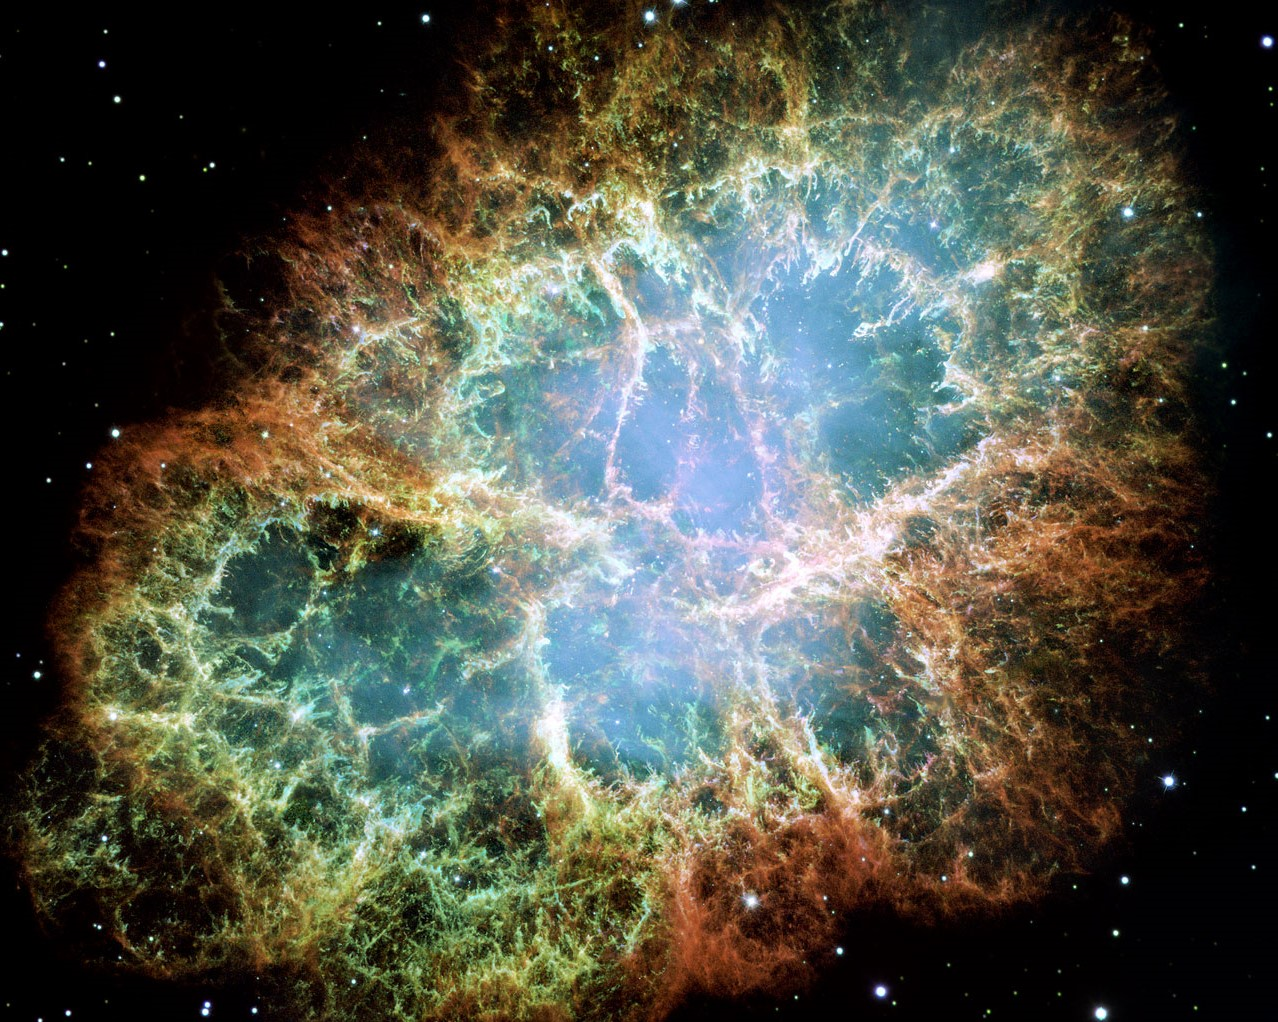
\includegraphics[width=\paperwidth, height =10cm]{../../Crab.jpg}}
    \end{figure}
\end{titlepage}

%%%%%%%%%%%%%%%%%%%%%%%
\tableofcontents

%%%%%%%%%%%%%%%%%%%%%%%%%%%%%%%%%%%%%% Part 1
\part{General Topological Spaces}

%%%%%%%%%%%%%%%%%%%%%%% - P1.Chapter 1
\chapter{\textsection Topological Spaces and Bases}

\section{Basic Definitions and Examples: Topological Spaces}


\begin{cust}[Motivating Example]
    Let $x = (x_1,...,x_n)$ and $y=(y_1,...,y_n)$ be points in $\R^n$. For $\varepsilon > 0$, we define an \Emph{$\varepsilon$-ball} around a point $x \in \R^n$ by \begin{equation*}
        B_{\varepsilon}(x) := \{y \in \R^n:d(x,y) < \varepsilon\}
    \end{equation*}
    where $d(x,y):=\sqrt{\sum_{i=1}^n(x_i-y_i)^2}$ is the usual Euclidean metric on $\R^n$. Next, we say that a subset $U$ of $\R^n$ is \Emph{open} if for every $x \in U$ there exists $\varepsilon > 0$ such that $B_{\varepsilon}(x) \subseteq U$. 

    Some facts about $\R^n$ is that $\emptyset$ and $\R^n$ are open, the union of an arbitrary collection of open sets is open, and the intersection of a finite collection of open sets is open. 
\end{cust}

\begin{defn}
    Let $X$ be a set. A collection $\mathcal{T} \subseteq \mathcal{P}(X)$ of subsets of $X$ is called a \Emph{topology on $X$} provided that the following three properties are satisfied: \begin{enumerate}
        \item $\emptyset \in \mathcal{T}$ and $X \in \mathcal{T}$.
        \item $\mathcal{T}$ is \Emph{closed under finite intersections}. That is, given any finite collection $U_1,...,U_n$ of sets in $\mathcal{T}$, their common intersection $U_1\cap ...\cap U_n$ is also an element of $\mathcal{T}$.
        \item $\mathcal{T}$ is \Emph{closed under arbitrary unions}. That is, if $\{U_{\alpha}\vert\alpha\in I\}$ is an indexed family of sets in $\mathcal{T}$ for index set $I$, then their union $\bigcup_{\alpha \in I}U_{\alpha}$ is also an element of $\mathcal{T}$.
    \end{enumerate}
    Given a set $X$ and a topology $\mathcal{T}$ on $X$, the pair $(X,\mathcal{T})$ is called a \Emph{topological space}. 


    The elements $U \in \mathcal{T}$ of a topology on $X$ are called \Emph{open subsets of $X$}, or simply \Emph{open sets}.
\end{defn}

\begin{eg}
    Let $X = \R^n$ and let \begin{equation*}
        \mathcal{T}_{usual} := \{U\subseteq \R^n:\forall x \in U,\exists\varepsilon > 0; B_{\varepsilon}(x) \subseteq U\},
    \end{equation*}
    As noted in the motivating example, $\mathcal{T}_{usual}$ forms a topology on $\R^n$. We call this the \Emph{usual or standard topology on $\R^n$}, and refer to $(\R^n,\mathcal{T}_{usual})$ as $\R^n$ with the usual topology. 

    In the case of $n = 1$, our definition above takes the following form: \begin{equation*}
        \mathcal{T}_{usual} := \{U \subseteq \R:\forall x\in U,\exists \delta >0; (x-\delta,x+\delta)\subseteq U\}
    \end{equation*}
    The nonempty open subsets of $\R_{usual}$ are precisely the open intervals and rays\--those intervals of the form $(a,b), (a,\infty),(-\infty,b), (-\infty,\infty) = \R$, for $a < b$\--with arbitrary unions of them.
\end{eg}

\begin{xca}
    Fix real numbers $a<b$. Explicitly show that the interval $(a,b)$ is open in $\R_{usual}$. Show that the interval $[a,b)$ is not open in $\R_{usual}$.
\end{xca}
\begin{cust}[Solution]
    Let $x \in (a,b)$. Then let $\delta = \min(|x-a|/2,|x-b|/2)$. It follows that for all $y \in (x-\delta, x+\delta)$, $|y-x| < \delta$, so in particular $y < \frac{b+x}{2} < b$ and $y > \frac{3x-a}{2} > a$, so $y \in (a,b)$. Hence, $(x-\delta,x+\delta) \subseteq (a,b)$. Thus, we have that $(a,b) \in \mathcal{T}_{usual}$. Next, consider $[a,b)$. Observe that for all $\varepsilon > 0$, there exists $a-\varepsilon < x < a$ by the density of $\R$. But, then $x \notin [a,b)$ as $x < a$, so in particular $(a-\varepsilon,a+\varepsilon) \nsubseteq [a,b)$ for all $\varepsilon > 0$, so $[a,b) \notin \mathcal{T}_{usual}$.
\end{cust}

\begin{eg}[Trivial Topologies]
    Let $X$ be any set. \begin{enumerate}
        \item Define $\mathcal{T}_{discrete} := \mathcal{P}(X)$. That is, $\mathcal{T}_{discrete}$ is the collection of all subsets of $X$. Then $\mathcal{T}_{discrete}$ is called the \Emph{discrete topology on $X$}.
        \item Let $X \neq \emptyset$. Define $\mathcal{T}_{indiscrete} :=\{\emptyset,X\}$. Then $\mathcal{T}_{indiscrete}$ is called the \Emph{indiscrete topology on $X$}, or sometimes the \Emph{trivial topology on $X$}.
    \end{enumerate}
\end{eg}


\begin{xca}
    Fix an arbitrary nonempty set $X$, and let $\mathcal{T}_{discrete}$ and $\mathcal{T}_{indiscrete}$ be the trivial topologies defined previously. Show that these are indeed topologies on $X$.
\end{xca}
\begin{cust}[Solution]
    Let $X$ be a nonempty set. Then by definition $\emptyset, X \in \mathcal{T}_{indiscrete}$, and since $\emptyset,X \subseteq X$, we have that $\emptyset, X \in \mathcal{P}(X) = \mathcal{T}_{discrete}$, so axiom $1$ holds for both sets. Next, let $\mathcal{C} \subseteq \mathcal{T}_{indiscrete}$ be an arbitrary subcollection. Then $\mathcal{C} = \{\emptyset\}$, $\mathcal{C} = \{X\}$, or $\mathcal{C} = \{\emptyset, X\}$. In any case $\bigcup\mathcal{C} = \emptyset$ or $X$, so $\bigcup\mathcal{C} \in \mathcal{T}_{indiscrete}$. Moroever, $\emptyset\cap X = \emptyset = \emptyset \cap \emptyset$ and $X\cap X = X$ are all in $\mathcal{T}_{indiscrete}$ so the set is closed under finite intersections. Thus $\mathcal{T}_{indiscrete}$ satisfies the axioms of a topology on $X$. Next, let $\mathcal{C} \subseteq \mathcal{T}_{discrete}$ be a subcollection. It follows that $\bigcup\mathcal{C} \subseteq X$, so $\bigcup\mathcal{C} \in \mathcal{P}(X) = \mathcal{T}_{discrete}$, so it is closed under arbitrary unions. Similarly, $\bigcap\mathcal{C} \in \mathcal{P}(X) = \mathcal{T}_{discrete}$, so $\mathcal{T}_{discrete}$ is closed under arbitrary intersections, and in particular it is closed under finite intersections.
\end{cust}

\begin{eg}
    Let $X = \{\triangle, \square, \lozenge,\heartsuit\}$. Define $$\mathcal{T}:=\{\emptyset, X, \{\triangle, \square, \lozenge\}, \{\lozenge,\heartsuit\},\{\lozenge\}\}$$
    Then $(X,\mathcal{T})$ is a topological space.
\end{eg}

\begin{eg}
    Working with $\R$ as the underlying set, define \begin{equation*}
        \mathcal{T}_{ray} :=\{(a,\infty):a\in \R\}\cup\{\emptyset,\R\}
    \end{equation*}
    Then $\mathcal{T}_{ray}$ is a topology on $\R$ we will call the ``ray topology."
\end{eg}

\begin{eg}
    Let $X$ be any nonempty set. Define \begin{equation*}
        \mathcal{T}_{co-finite} := \{U \subseteq X:X\backslash U\text{ is finite}\}\cup\{\emptyset\}
    \end{equation*}
    Then $\mathcal{T}_{co-finite}$ is called the \Emph{co-finite topology} on $X$.
\end{eg}

\begin{eg}
    Let $X$ be any nonempty set. Define \begin{equation*}
        \mathcal{T}_{co-uncountable} := \{U\subseteq X:X\backslash U\text{ is countable}\}\cup\{\emptyset\}
    \end{equation*}
    Then $\mathcal{T}_{co-countable}$ is called the \Emph{co-countable topology} on $X$.
\end{eg}

\begin{eg}
    Let $X$ be a onempty set, and fix an element $p \in X$. Define \begin{equation*}
        \mathcal{T}_p :=\{U\subseteq X:p \in U\}\cup\{\emptyset\}
    \end{equation*}
    Then $\mathcal{T}_p$ is called the \Emph{particular point topology at $p$} on $X$.
\end{eg}

\begin{xca}
    Under what assumptions on the set $X$ does $\mathcal{T}_{co-finite} = \mathcal{T}_{co-countable}$? We must place the assumption that $X$ is itself finite.
\end{xca}


\subsection{Comparing Topologies}


\begin{defn}
    Let $X$ be a set, and suppose $\mathcal{T}_1$ and $\mathcal{T}_2$ are topologies on $X$. We say that $\mathcal{T}_1$ \Emph{refines} $\mathcal{T}_2$, or that $\mathcal{T}_1$ is \Emph{finer than} $\mathcal{T}_2$, if $\mathcal{T}_1 \supseteq \mathcal{T}_2$. In other words, a topology with more open sets is finer than a topology with fewer open sets.

    This is equivalent to stating that $\mathcal{T}_2$ is \Emph{refined by} $\mathcal{T}_1$, or that $\mathcal{T}_2$ is \Emph{coarser than} $\mathcal{T}_1$.
\end{defn}


\begin{eg}
    For the $\R$, we have: \begin{equation*}
        \mathcal{T}_{discrete} \text{ refines }\mathcal{T}_{usual}, \text{ which refines }\mathcal{T}_{ray}, \text{ which refines }\mathcal{T}_{indiscrete}
    \end{equation*}
\end{eg}


\begin{xca}
    Fix a nonempty set $X$. Show that $\mathcal{T}_{co-finite}$ is coarser than $\mathcal{T}_{co-countable}$. Let $U \in \mathcal{T}_{co-finite}$. Then we have that $X\backslash U$ is finite, so in particular it is countable. Hence $U \in \mathcal{T}_{co-countable}$ so $\mathcal{T}_{co-finite} \subseteq \mathcal{T}_{co-countable}$.
\end{xca}

\begin{rmk}
    Given two topologies $\mathcal{T}_1$ and $\mathcal{T}_2$ of a set $X$, it may be that neither refines the other. In this case, we sometimes say that $\mathcal{T}_1$ and $\mathcal{T}_2$ are \Emph{incomparable} topologies.
\end{rmk}

\begin{eg}
    $\mathcal{T}_{usual}$ and $\mathcal{T}_7$ are incomparable topologies on $\R$. To see this, note that $(1,2)$ is open in $\mathcal{T}_{usual}$, but it does not contain $7$ so it is not open in $\mathcal{T}_7$. This shows that $\mathcal{T}_{usual}\nsubseteq \mathcal{T}_7$, so $\mathcal{T}_7$ does not refine $\mathcal{T}_{usual}$. 

    On the other hand, the set $\{\pi,7\}$ is open in $\mathcal{T}_7$ since it contains $7$, but it is not open in $\mathcal{T}_{usual}$. This shows that $\mathcal{T}_7 \nsubseteq \mathcal{T}_{usual}$, so $\mathcal{T}_{usual}$ does not refine $\mathcal{T}_7$.
\end{eg}



\section{Bases of a Topology}

Often we cannot specify a Topology explicitly in terms of its open sets. Instead, we wish to find a smaller collection of sets we can specify explicitly which can then be used to populate a topology given certain axioms. 

\begin{xca}
    Let $X$ be a nonempty set, and let $\mathcal{B} = \{\{x\}:x \in X\}$. Show that if $\mathcal{T}$ is a topology on $X$ and $\mathcal{B}\subseteq \mathcal{T}$, then $\mathcal{T}$ is the discrete topology on $X$. Let $\mathcal{T}$ be a topology on $\R$ containing all of the usual open intervals. Is $\mathcal{T}$ the usual topology? Not necessarily, as it can be the discrete topology. Now, let $U \in \mathcal{P}(X)$. Then, let $\mathcal{C} = \{\{x\}:x\in U\} \subseteq \mathcal{T}$. Then since $\mathcal{T}$ is a topology we have that $U = \bigcup\mathcal{C}\in \mathcal{T}$. Hence $\mathcal{T} = \mathcal{P}(X)$ is the discrete topology on $X$.
\end{xca}

\begin{rmk}
    If $\mathcal{A}$ is a collection of sets, then \begin{equation*}
        \bigcup\mathcal{A} := \bigcup\limits_{X\in\mathcal{A}}X
    \end{equation*}
\end{rmk}


\begin{defn}
    Let $X$ be a set. A collection of sets $\mathcal{B} \subseteq \mathcal{P}(X)$ is called a \Emph{basis on $X$} if the following two properties hold:\begin{enumerate}
        \item \Emph{$\mathcal{B}$ covers $X$}. That means: $\forall x \in X, \exists B \in \mathcal{B}: x\in B$. Or, more consicely $X = \bigcup\mathcal{B}$.
        \item $\forall B_1,B_2 \in \mathcal{B}$, $\forall x \in B_1\cap B_2$, $\exists B \in \mathcal{B}$ such that $x \in B \subseteq B_1\cap B_2$.
    \end{enumerate}
\end{defn}


\begin{defn}
    Let $X$ be a set and $\mathcal{B}$ a basis on $X$. We define \begin{equation*}
        \mathcal{T}_{\mathcal{B}} :=\{\bigcup \mathcal{C}:\mathcal{C}\subseteq \mathcal{B}\}\cup\{\emptyset\}
    \end{equation*}
    Then $\mathcal{T}_{\mathcal{B}}$ is called the \Emph{topology generated by $\mathcal{B}$}. Note $\emptyset \subseteq \mathcal{B}$ and $\bigcup\emptyset = \emptyset$, so technically speaking we do not need to add it explicitly.
\end{defn}


\begin{eg}
    \leavevmode
    \begin{enumerate}
        \item Let $X$ be a set, and let $\mathcal{B} = \{\{x\}:x \in X\}$. Then $\mathcal{B}$ is a basis on $X$, and $\mathcal{T}_{\mathcal{B}}$ is the discrete topology.
        \item The collection $\mathcal{A} = \{(a,\infty)\subseteq \R:a \in \R\}$ of open rays is a basis on $\R$, for somewhat trivial reasons. $\mathcal{A}$ coverse $\R$ since for example $x \in (x-1,\infty)$ for any $x$. Moreover, given any two elements of $\mathcal{A}$, their intersection is again an element of $\mathcal{A}$ (i.e. $\mathcal{A}$ is closed under pairwise intersections), and therefore it follows inductively that the intersection of finitely many elements of $\mathcal{A}$ is again an element of $\mathcal{A}$. This makes the second property in the definition of a basis immediately satisfied. 
        \item The collection $\mathcal{B} = \{(a,b) \subseteq \R:a <b\}$ of open intervals is a basis on $\R$.
        \item The collection $\mathcal{B}_2 = \{B_{\varepsilon}(x) \subseteq \R^2:x \in \R^2,\varepsilon > 0\}$ is a basis on $\R^2$.
        \item The collection $\mathcal{B} = \{[a,b)\subseteq \R:a < b\}$ of ``half-open" intervals is a basis on $\R$. So is $\mathcal{B}' = \{(a,b]\subseteq \R:a<b\}$.
        \item Let $(X_1,\mathcal{T}_1)$ and $(X_2,\mathcal{T}_2)$ be topological spaces, and define: \begin{equation*}
                \mathcal{B} = \mathcal{T}_1\times \mathcal{T}_2 = \{U\times V\subseteq X_1\times X_2: U\in \mathcal{T}_1,V\in\mathcal{T}_2\}
        \end{equation*}
            Then $\mathcal{B}$ is a basis on $X_1\times X_2$.
            \begin{proof}
                First, since $X_1\times X_2 \in \mathcal{T}_1\times \mathcal{T}_2$ as they are topologies, we have that $\mathcal{T}_1\times \mathcal{T}_2$ covers $X_1\times X_2$. Next, for any $U_1\times V_1, U_2\times V_2 \in \mathcal{T}_1\times \mathcal{T}_2$, we have that $(U_1\times V_1)\cap(U_2\times V_2) = (U_1\cap U_2)\times (V_1\cap V_2)$, where $U_1\cap U_2 \in \mathcal{T}_1$ and $V_1\cap V_2 \in \mathcal{T}_2$, so $(U_1\cap U_1)\times (V_1\cap V_2) \in \mathcal{T}_1\times \mathcal{T}_2$. Hence, $\mathcal{B} = \mathcal{T}_1\times \mathcal{T}_2$ is indeed a basis on $\mathcal{B}$.
            \end{proof}
        \item The collection \begin{equation*}
                \mathcal{B} = \{(a,b)\times (c,d) \in \R^2: a < b, c < d\}
        \end{equation*}
            is a basis on $\R^2$.
            \begin{proof}
                Note that for all $(x,y) \in \R^2$, $(x,y) \in (x-\delta,x+\delta)\times (y-\delta,y+\delta) \in \mathcal{B}$ for $\delta > 0$ so $\mathcal{B}$ covers $\R^2$. Moreover, for $(a_1,b_1)\times (c_1,d_1),(a_2,b_2)\times(c_2,d_2) \in \mathcal{B}$, and suppose $((a_1,b_1)\times(c_1,d_1))\cap((a_2,b_2)\times(c_2,d_2)) \neq \emptyset$. Let $x \in (a_1,b_1) \cap(a_2,b_2)$ and $y \in (c_1,d_1)\cap(c_2,d_2)$. Then choose $\delta_1 = \frac{1}{2}\min\{|x-a_1|,|x-b_1|,|x-a_2|,|x-b_2|\}$ and $\delta_2 = \frac{1}{2}\min\{|y-c_1|,|y-d_1|,|y-c_2|,|y-d_2|\}$. It follows that $(x-\delta_1,x+\delta_1) \subseteq (a_1,b_1)\cap(a_2,b_2)$ and $(y-\delta_2,y+\delta_2)\subseteq (c_1,d_1)\cap(c_2,d_2)$. Hence, we have that $$(x,y) \in (x-\delta_1,x+\delta_1)\times(y-\delta_2,y+\delta_2) \subseteq ((a_1,b_1)\times(c_1,d_1))\cap((a_2,b_2)\times(c_2,d_2)) \subseteq \mathcal{B}$$ so the second axiom is satisied by $\mathcal{B}$. Hence, $\mathcal{B}$ is a basis on $\R^2$. 

                Let $\mathcal{C} = \mathcal{T}_{usual}\times\mathcal{T}_{usual}$. Then note that for all $a < b$, $(a,b) \in \mathcal{T}_{usual}$ so $\mathcal{B} \subseteq \mathcal{C}$ by definition. However, note that $((1,2)\cup(3,4)) \times (1,2) \in \mathcal{C}$ while it is not in $\mathcal{B}$ so $\mathcal{C} \nsubseteq \mathcal{B}$, and consequently $\mathcal{B} \neq \mathcal{C}$.
            \end{proof}
            \item A topology $\mathcal{T}$ on a set $X$ is itself a basis on $X$: First, $X \in \mathcal{T}$ anso $\mathcal{T}$ covers $X$. Second, the intersection of two sets in $\mathcal{T}$ is again in $\mathcal{T}$ since $\mathcal{T}$ is closed under finite intersections, and so the second property in the definition of a basis is trivially satisfied. 
    \end{enumerate}
\end{eg}

\begin{proof}[Proof that $\mathcal{T}_{\mathcal{B}}$ is a Topology]
    (1) $\emptyset \in \mathcal{T}_{\mathcal{B}}$ by definition, and $X \in \mathcal{T}_{\mathcal{B}}$ since $\mathcal{B}$ covers $X$, so $X = \bigcup\mathcal{B} \in \mathcal{T}_{\mathcal{B}}$.

    
    (2) $\mathcal{T}_{\mathcal{B}}$ is closed under arbitrary unions. Let $\{V_{\alpha}:\alpha \in I\}$ be an indexed family of elements in $\mathcal{T}_{\mathcal{B}}$. By definition of $\mathcal{T}_{\mathcal{B}}$, for each $\alpha \in I$ there exists a collection $\mathcal{C}_{\alpha} \subseteq \mathcal{B}$ such that $V_{\alpha} = \bigcup\mathcal{C}_{\alpha}$. Immediately we can see that \begin{equation*}
        \bigcup\limits_{\alpha\in I}\left(\bigcup\mathcal{C}_{\alpha}\right) = \bigcup\left(\bigcup\limits_{\alpha \in I}\mathcal{C}_{\alpha}\right) \in \mathcal{T}_{\mathcal{B}},
    \end{equation*}
    where the last set is an element of $\mathcal{T}_{\mathcal{B}}$ since $\bigcup_{\alpha \in I}\mathcal{C}_{\alpha} \subseteq \mathcal{B}$. 


    (3) $\mathcal{T}_{\mathcal{B}}$ is closed under finite intersections. Fix two elements $U = \bigcup\mathcal{A}$ and $V = \bigcup\mathcal{C}$ in $\mathcal{T}_{\mathcal{B}}$. We want to show that $U\cap V \in \mathcal{T}_{\mathcal{B}}$. First note that $x \in U\cap V$ if and only if there exists $A \in \mathcal{A}$ and $C \in \mathcal{C}$ such that $x \in A\cap C$. Hence \begin{equation*}
        U\cap V = \left(\bigcap\mathcal{A}\right)\cup\left(\bigcap\mathcal{C}\right) = \bigcup\{A\cap C:A\in\mathcal{A},C\in\mathcal{C}\}
    \end{equation*}
    Since $\mathcal{T}_{\mathcal{B}}$ is closed under arbitrary unions by (2), it is sufficient to show that \begin{equation*}
        \{A\cap C:A \in \mathcal{A},C\in\mathcal{C}\}\subseteq \mathcal{T}_{\mathcal{B}}
    \end{equation*}
    So fix $A\cap C$ for some $A \in \mathcal{A}$ and $C \in \mathcal{C}$. If $A\cap C$ is nonempty, then for a given $x \in A\cap C$ there exists $B_x \in \mathcal{B}$ such taht $x \in B_x \subseteq A\cap C$ since $\mathcal{B}$ is a basis. As this applies for all $x \in A\cap C$, we have that \begin{equation*}
        A\cap C\subseteq \left[\bigcup\limits_{x\in A\cap C}B_x\right]\subseteq A\cap C
    \end{equation*}
    so we have that \begin{equation*}
        A\cap C = \left[\bigcup\limits_{x\in A\cap C}B_x\right] \in \mathcal{T}_{\mathcal{B}}
    \end{equation*}
    On the other hand, if $A\cap C$ is empty then it is in $\mathcal{T}_{\mathcal{B}}$ by (1).
\end{proof}


\begin{defn}
    Let $X$ be a set and $\mathcal{B}$ a basis on $X$. Define \begin{equation*}
        \mathcal{T}_{\mathcal{B}}' := \{U\subseteq X:\forall x \in U,\exists B_x \in \mathcal{B};x \in B_x \subseteq U\}
    \end{equation*}
\end{defn}
\begin{proof}[$\mathcal{T}_{\mathcal{B}}'$ Defines a Topology on $X$]
    (To be finished)
\end{proof}


\begin{xca}
    Prove that the two definitions for the topology generated by a basis $\mathcal{B}$ are equivalent. 
\end{xca}
\begin{proof}
    (To be finished)
\end{proof}


\begin{rmk}
    Observe that $\mathcal{B} \subseteq \mathcal{T}_{\mathcal{B}}$ and $\mathcal{B} \subseteq \mathcal{T}_{\mathcal{B}}'$. Indeed, fixing some $U \in \mathcal{B}$, $U = \bigcup\{U\} \in \mathcal{T}_{\mathcal{B}}$, so $\mathcal{B} \subseteq \mathcal{T}_{\mathcal{B}}$. On the other hand for all $x \in U$, $x \in U \subseteq U$, so $U \in \mathcal{T}_{\mathcal{B}}'$. Hence $\mathcal{B}\subseteq \mathcal{T}_{\mathcal{B}}'$.

    Hence, all basis elements are open sets, so we often call them the \Emph{basic open sets} of the topology.
\end{rmk}

\begin{eg}
    \leavevmode
    \begin{enumerate}
        \item The basis consisting of all singletons in a set $X$ generates the discrete topology on $X$.
        \item The basis consisting of all the open intervals in $\R$ generates the usual or Euclidean topology on $\R$.
        \item The basis consisting of all open balls in $\R^2$ generates the usual topology on $\R^2$.
        \item Given a topology $\mathcal{T}$ on a set $X$, $\mathcal{T}$ is itself a basis for itself.
    \end{enumerate}
\end{eg}

\begin{defn}
    Let $\mathcal{B} := \{[a,b)\subseteq\R:a <b\}$. Then $\mathcal{B}$ is a basis on $\R$. The topology $\mathcal{S} := \mathcal{T}_{\mathcal{B}}$ it generates is called the \Emph{lower limit topology on $\R$}, and the corresponding topological space $(\R,\mathcal{S})$ is called the \Emph{Sorgenfrey line}. 
\end{defn}

\begin{lem}
    Let $\mathcal{B}_1$ and $\mathcal{B}_2$ be two bases on a set $X$, then $\mathcal{T}_{\mathcal{B}_1} \subseteq \mathcal{T}_{\mathcal{B}_2}$ if and only if for every $x \in X$ and $B_1 \in \mathcal{B}_1$ containing $x$, there is a $B_2 \in \mathcal{B}_2$ such taht $x \in B_2 \subseteq B_1$.
\end{lem}
\begin{proof}
    We will proceed using the notation specified in the lemma.

    Assuming that $\mathcal{T}_{\mathcal{B}_1}\subseteq \mathcal{T}_{\mathcal{B}_2}$, fix an element $x \in X$ and a basic open set $B_1 \in \mathcal{B}_1$ such that $x \in B_1$. Then $B_1 \in \mathcal{T}_{\mathcal{B}_1}$, so in particular $B_1 \in \mathcal{T}_{\mathcal{B}_2}$, so by definition there exists $B_2 \in \mathcal{B}_2$ such that $x \in B_2 \subseteq B_1$.


    Conversely, assuming that for all $x \in X$ and $B_1 \in \mathcal{B}_1$ containing $x$, there is a $B_2 \in \mathcal{B}_2$ such that $x \in B_2 \subseteq B_1$, let $U \in \mathcal{T}_{\mathcal{B}_1}$ be an arbitrary open set. Then, note that by assumption $\mathcal{B}_1 \subseteq \mathcal{T}_{\mathcal{B}_2}$, and as $U \in \mathcal{T}_{\mathcal{B}_1}$ there exists a subcollection $\mathcal{C} \subseteq \mathcal{B}_1$ of basic open sets such that $U = \bigcup\{\mathcal{C}\}$. However, $\mathcal{C} \subseteq \mathcal{B}_1\subseteq\mathcal{T}_{\mathcal{B}_2}$, so as $\mathcal{T}_{\mathcal{B}_2}$ is closed under arbitrary unions we have that $U =\bigcup\{\mathcal{C}\} \in \mathcal{T}_{\mathcal{B}_2}$. Consequently we find that $\mathcal{T}_{\mathcal{B}_2}$ is finer than $\mathcal{T}_{\mathcal{B}_1}$.
\end{proof}

\begin{cor}{}{basisCond}
    Let $(X,\mathcal{T})$ be a topological space and $\mathcal{B}$ a basis on $X$. Then $\mathcal{B}$ generates $\mathcal{T}$ if and only if \begin{enumerate}
        \item $\mathcal{B}\subseteq \mathcal{T}$; and 
        \item for every $U \in \mathcal{T}$ and every $x \in U$, there is a $B \in \mathcal{B}$ such that $x \in B\subseteq U$
    \end{enumerate}
\end{cor}
\begin{proof}

    Assuming that $\mathcal{B}$ generates $\mathcal{T}$ we have that all basic open sets $B \in \mathcal{B}$ are open sets in $\mathcal{T}$. Indeed, for all $x \in B$, $x \in B \subseteq B$, so by definition of the topology generated by $\mathcal{B}$ we have that $B \in \mathcal{T}$ is open. Consequently $\mathcal{B} \subseteq \mathcal{T}$ is a subcollection of open sets. Then, by definition of the topology generated by the basis $\mathcal{B}$, for all $U \in \mathcal{T}$ and every $x \in U$, there exists $B \in \mathcal{B}$ such taht $x \in B\subseteq U$, so the second condition is immediately satisfied.


    On the other hand, assuming that the two conditions are satisfied, we have that $\{\bigcup\{\mathcal{C}\}:\mathcal{C}\subseteq \mathcal{B}\} \subseteq \mathcal{T}$ since $\mathcal{B}\subseteq \mathcal{T}$ and $\mathcal{T}$ is closed under arbitrary unions. Moreover, for every $U \in \mathcal{T}$ and each $x \in U$ there exists $B_x \in \mathcal{B}$ such that $x \in B_x \subseteq U$. Hence, we find that $U = \bigcup_{x \in U}B_x$, so $U \in \{\bigcup\{\mathcal{C}\}:\mathcal{C}\subseteq\mathcal{B}$. It follows immediately that $\mathcal{T} \subseteq \{\bigcup\{\mathcal{C}\}:\mathcal{C}\subseteq\mathcal{B}$, so as both inclusions hold $\mathcal{T}$ is the topology generated by $\mathcal{B}$.
\end{proof}

\begin{xca}
    I claim that the sets $\mathcal{B}_1 = \{(a,\infty): a\in \R\}\cup\{(-\infty,a):a\in\R\}\cup\{\emptyset\}$ and $\mathcal{B}_2 = \{(p,q):p,q\in\Q, p < q\}$ are bases for the usual topology on $\R$.
\end{xca}
\begin{proof}
    (To be completed)
\end{proof}


\begin{xca}
    I claim that the sets $\mathcal{B}_1 =  \{\emptyset\}\cup\{S_{\varepsilon}(\vec{x}) \subseteq \R^n:\vec{x} \in \R^n, \varepsilon >0\}$ and $\mathcal{B}_2 = \{\pi_i^{-1}(U) \subseteq \R^n:U \in \mathcal{T}_{usual}\}$ where $S_{\varepsilon}(\vec{x}) := (x_1-\varepsilon,x_1+\varepsilon)\times ... \times(x_n-\varepsilon,x_n+\varepsilon$, $\pi_i:\R^n\rightarrow \R$ by $\pi_i(\vec{x}) = x_i$, and $\mathcal{T}_{usual}$ is the usual topology on $\R$.
\end{xca}
\begin{proof}
    (To be completed)
\end{proof}


\begin{xca}
    The lower limit topology on $\R$ refines the usual topology on $\R$, strictly.
\end{xca}
\begin{proof}
    (To be completed)
\end{proof}




\section{Closed Sets and Closures}


\begin{defn}
    A sequence $\{x_n\}_{n=1}^{\infty}$ is said to \Emph{converge} to a point $x \in \R^n$ if for every $\epsilon > 0$ there is a number $N \in \N$ such that $x_n \in B_{\epsilon}(x)$ for all $n \geq N$.
\end{defn}

\begin{rmk}
    It is common to refer to the portion of a sequence $\{x_n\}_{n=1}^{\infty}$ after some index $N$ (that is, the sequence $\{x_n\}_{n=N+1}^{\infty}$) as a \Emph{tail} of the sequence. In this language, one would phrase the above definition as ``for every $\epsilon > 0$ there is a tail of the sequence inside $B_{\epsilon}(x)$."
\end{rmk}

\begin{rmk}
    By definition of the usual topology on $\R^n$, this definition is equivalent to stating that for any open neighborhood $U$ of $x$, there is a tail of the sequence in $U$.
\end{rmk}


\subsection{Closures}

\begin{defn}
    Let $(X,\mathcal{T})$ be a topological space, and let $A \subseteq X$. We define the \Emph{closure of $A$ in $(X,\mathcal{T})$}, which we denote $\overline{A}$, by: \begin{equation*}
        x \in \overline{A}\text{ if and only if for every open set $U$ containing $x$, } U\cap A\neq \emptyset
    \end{equation*}
    Or, in symbols: \begin{equation*}
        \overline{A} = \{x \in X:\forall U\in\mathcal{T};U \in N(x), U\cap A\neq \emptyset\}
    \end{equation*}
\end{defn}


\begin{prop}
    Let $(X,\mathcal{T})$ be a topological space and let $A,B\subseteq X$. Then:\begin{enumerate}
        \item $A\subseteq \overline{A}$
        \item $\overline{\overline{A}} = \overline{A}$ (That is, taking closures is an \Emph{idempotent} operation)
        \item $\overline{A\cup B} = \overline{A}\cup\overline{B}$
        \item $X\backslash A$ is open if, and only if, $\overline{A} = A$
        \item Trivially, $\overline{\emptyset} = \emptyset$ and $\overline{X} = X$
    \end{enumerate}
\end{prop}
\begin{proof}
    \leavevmode
    \begin{enumerate}
        \item Let $a \in A$. Then for all open sets $U \in N(a)$, $a \in U$ so $a \in U\cap A$ and hence $U\cap A \neq \emptyset$. Thus as $U$ was an arbitrary neighborhood of $a$, $a \in \overline{A}$ and hence $A \subseteq \overline{A}$.
        \item By the first point we have the inclusion $\overline{A} \subseteq \overline{\overline{A}}$. Now, let $x \in \overline{\overline{A}}$. Then by definition for all open sets $U \in N(x)$, $U \cap \overline{A} \neq \emptyset$, so there is at least one point $y \in U \cap \overline{A}$. Since $y \in \overline{A}$ we again have by definition that for all open sets $V \in N(y)$, $V \cap A \neq \emptyset$. But $y \in U$ an open set implies $U \in N(y)$, so we must have that $U \cap A \neq \emptyset$. Therefore by definition $x \in \overline{A}$, so $\overline{\overline{A}} \subseteq \overline{A}$. Consequently, we conclude that $\overline{A} = \overline{\overline{A}}$.
        \item First let $x \in \overline{A\cup B}$. Then for all open sets $U \in N(x)$, we have that $U \cap(A\cup B) \neq \emptyset$. Then I claim that either $U\cap A \neq \emptyset$ for all $U \in N(x)$ or $U\cap B \neq \emptyset$ for $U \in N(x)$. If it is true for both $A$ and $B$ then $x \in \overline{A}$ and $x \in \overline{B}$, so $x \in \overline{A}\cup\overline{B}$ so we are done. Hence, suppose without loss of generality that there exists $U \in N(x)$ such that $U\cap B = \emptyset$. Then since $U\cap(A\cup B) \neq \emptyset$ we must have that $U \cap A\neq \emptyset$. Now, towards a contradiction suppose there exists $V \in N(x)$ such that $V\cap A = \emptyset$. But then $V\cap U \in N(x)$ is an open set since open sets are closed under finite intersections, and $(V\cap U)\cap A = \emptyset$ and $(V\cap U)\cap B = \emptyset$, which implies $(V\cap U)\cap (A\cup B) = \emptyset$, a contradiction. Therefore, we must have that for all open sets $V \in N(x)$, $V\cap A \neq \emptyset$, so $x \in \overline{A}$. Consequently, we find that $x \in \overline{A}\cup\overline{B}$, so $\overline{A\cup B} \subseteq \overline{A}\cup\overline{B}$.

            On the other hand, let $y \in \overline{A} \cup \overline{B}$, and without loss of generality suppose $y \in \overline{A}$. Then for all open sets $U \in N(y)$ we have $U \cap A \neq \emptyset$, so in particular $U \cap (A\cup B) \neq \emptyset$. Therefore by definition $y \in \overline{A\cup B}$ so $\overline{A\cup B}\supseteq \overline{A}\cup\overline{B}$, and we conclude the equality $$\overline{A\cup B} = \overline{A}\cup\overline{B}$$

        \item Firstly, suppose that $X\backslash A$ is open, and let $a \in \overline{A}$. Towards a contradiction suppose $a \in X\backslash A$. But since $X\backslash A$ is open and $a \in \overline{A}$, we would then need that $(X\backslash A) \cap A \neq \emptyset$, which is a contradiction as $(X\backslash A)\cap A = \emptyset$. Therefore, $a \notin X\backslash A$, so $a \in A$. Hence $\overline{A} \subseteq A$, and by our first remark we obtain equality with $A = \overline{A}$.

            Conversely, suppose that $\overline{A} = A$, and let $x \in X\backslash A$. Then since $x \notin A = \overline{A}$, there must exist $U_x \in N(x)$ such that $U_x \cap A = \emptyset$. Consequently, $U_x$ is containd in $X\backslash A$. But this applies for all $x$ of $X\backslash A$, so \begin{equation*}
                \bigcup_{x \in X\backslash A}U_x = X\backslash A
            \end{equation*}
            so we must have that $X\backslash A$ is open as it is the union of open sets, and open sets are closed under arbitrary unions.
    \end{enumerate}
\end{proof}


\begin{eg}
    \leavevmode
    \begin{enumerate}
        \item Working in $\R_{usual}$, the closure of an open interval $(a,b)$ is the corresponding ``closed" interval $[a,b]$.

            To see this, by the first point of the previous proposition $(a,b) \subseteq \overline{(a,b)}$. We must show that $a,b \in \overline{(a,b)}$. Let $U$ be an open set containing $a$. Then there is an $\epsilon > 0$ such that $B_{\epsilon}(a) = (a-\epsilon,a+\epsilon) \subseteq U$. Let $\delta = \min\{\epsilon,b-a\}$. Then $a+\delta/2 \in U\cap (a,b)$, as required. The proof of $b$ is analogous. This established that $[a,b] \subseteq \overline{(a,b)}$.

            Finally, if $x \in \R\backslash[a,b]$, the set $(-\infty,a)\cup(b,\infty)$ is an open set containing $x$ disjoint from $(a,b)$, witnessing that $x \notin \overline{(a,b)}$.
        \item Again in $\R_{usual}$, show the following straightforward facts for any $a<b<c$:\begin{enumerate}
                \item $\overline{\{a\}} = \{a\}$
                \item $\overline{[a,b)} = [a,b]$
                \item $\overline{(a,b)\cup(b,c)} = [a,c]$
                \item $\overline{[a,b]} = [a,b]$
                \item Let $A = \{1/n:n \in \N\}$. Then $\overline{A} = A\cup\{0\}$.
                \item More generally, if $\{x_n\}_{n=1}^{\infty}$ is a sequence that converges to a point $x \in \R$, then $\overline{\{x_n:n \in \N\}} = \{x_n:n\in\N\}\cup\{x\}$.
        \end{enumerate}
            \begin{proof}
                \leavevmode
                \begin{enumerate}
                    \item Note that $\R\backslash \{a\} = (-\infty,a)\cup(a,\infty)$ which is open, so by our previous proposition $\overline{\{a\}} = \{a\}$.
                    \item Note that by a similar argument to the case of $(a,b)$, $[a,b] \subseteq \overline{[a,b)}$. Similarly, for all $x \notin [a,b]$, $x \in (-\infty,a)\cup(b,\infty)$, which is disjoint from $[a,b)$, so $x \notin \overline{[a,b)}$. Hence $\overline{[a,b)} = [a,b]$.
                    \item By our previous proposition we have that $$\overline{(a,b)\cup(b,c)} = \overline{(a,b)}\cup\overline{(b,c)} = [a,b]\cup[b,c] = [a,c]$$
                    \item Note $\R\backslash[a,b] = (-\infty,a)\cup(b,\infty)$, which is open, so by our previous proposition $\overline{[a,b]} = [a,b]$.
                    \item First, note that for all $B_{\varepsilon}(0)$, there exists $N \in \N$ such that $\frac{1}{N} < \varepsilon$, so $\frac{1}{N} \in B_{\varepsilon}(0)$, and hence $B_{\varepsilon}(0) \cap A \neq \emptyset.$ Therefore we have that $\overline{A} \supseteq A \cup \{0\}$. Now, suppose $x \in \overline{A}\backslash (A\cup\{0\})$. If $x < 0$ then $x \in (-\infty, 0)$, which is disjoint from $A$, and hence a contradiction. If $x > 1$ then again $x \in (1,\infty)$ which is disjoint from $A$. On the other hand $0 < x < 1$. Then, let $B = \{n \in \N: 1/n < x\}$. By the Archimedean property of $\R$ $B$ is non-empty, so by the well-ordering of $\N$ there exists a least element $m \in B$, such that $1/m < x$. Then $1/m < x < 1/(m-1)$. But then $x \in (1/m,1/(m-1))$ which is an open set disjoint from $A$, and hence a contradiction. Thus, $\overline{A}\backslash (A\cup\{0\}) = \emptyset$, so $\overline{A} = A\cup\{0\}$.
                    \item Let $\{x_n\}_{n=1}^{\infty}$ be a sequence that converges to a point $x \in \R$. Then for all $B_{\epsilon}(x)$ there exists $N \in \N$ such that for all $n \geq N$, $x_n \in B_{\epsilon}(x)$, so in particular $B_{\epsilon}(x) \cap \{x_n:n\in\N\} \neq \emptyset$. Thus $\{x_n:n\in\N\}\cup\{x\} \subseteq \overline{\{x_n:x\in\N\}}$. Now, towards a contradiction let $a \in \overline{\{x_n:x\in\N\}}\backslash (\{x_n:n\in\N\}\cup\{x\})$. Then for all $\varepsilon > 0$, $B_{\varepsilon}(a)\cap\{x_n:n\in\N\} \neq \emptyset$. We shall employ the Principle of Recursive Definition to define a subsequence $\{a_n\}$ of $\{x_n\}$. Define a function $h:\Z_+\rightarrow \N$ by $h(1) = \min\{n \geq 1: x_n \in B_1(a)\}$, and \begin{equation*}
                            h(i) = \min\{n>h(i-1):x_n \in B_{1/i}(a)\}
                    \end{equation*}
                        Then by the the principle of recursive definition we have a sequence $\{h(n)\}_{n=1}^{\infty}$ of indices, such that the subsequence $\{x_{h(n)}\}_{n=1}^{\infty}$ satisfies $x_{h(n)} \in B_{1/n}(a)$ for each $n$. It follows that $\lim\limits_{n\rightarrow \infty}x_{h(n)} = a$, but $\{x_{h(n)}\}$ is a convergent subsequence of a convergent series, so it must converge to $x$ as well. But, by assumption $x \neq a$, which is a contradiction since metric spaces are Hausdorff. Thus, we conclude that $\overline{\{x_n:n\in\N\}} = \{x_n:n\in\N\}\cup\{x\}$ as desired.
                \end{enumerate}
            \end{proof}
        \item Generalizing our first example, let $x\in\R^n$ and $\epsilon > 0$. Then the closure of an $\epsilon$-ball $B_{\epsilon}(x)$ in $\R^n_{usual}$ is $\overline{B_{\epsilon}}(x) = \{y\in \R^n:d(x,y)\leq \epsilon\}$.
        \item It may seem as though any singleton is its own closure, but this need not be true in all topological spaces. For example, let $X = \{0,1\}$ and let $\mathcal{T} = \{\emptyset, X, \{1\}\}$. Then $(X,\mathcal{T})$ is a topological space, and $\overline{\{1\}} = X$. 
        \item For another exmaple of the same idea, let $(\R,\mathcal{T}_{ray})$ be the reals with the ray topology defined previously. Then $\overline{\{7\}} = (-\infty,7]$. 
        \item In $(X,\mathcal{T}_{discrete})$, for any $A \subseteq X$, $\overline{A} = A$. In other words, every set is its own closure.
        \item In $(X,\mathcal{T}_{indiscrete})$, for any nonempty $A \subseteq X$, $\overline{A} = X$.
        \item In the Sorgenfrey line:\begin{enumerate}
                \item Show that singletons are their own closures. (Since singletons are their own closures in $\R_{usual}$, the complement of singletons is open which implies the complement of singletons is open in the Sorgenfrey line as it is finer than $\R_{usual}$. Hence, singletons must be equal to their own closures)
                \item For any $a<b \in \R$, show that $\overline{[a,b]} = [a,b]$ and $\overline{[a,b)} = [a,b)$. The complement of both $[a,b]$ and $[a,b)$ is open in the Sorgenfrey line, so they are equal to their closures. Note that this implies that all open sets are clopen in the Sorgenfrey line.
                \item On the other hand, $\overline{(a,b)} = [a,b)$. Indeed, first of all if $x \geq b$, then $[x,x+1)$ is an open set containing $x$ and disjoing from $(a,b)$, so $x \notin \overline{(a,b)}$. Second of all if $x < a$, then $[x-1, x+\frac{a-x}{2})$ is an open set containing $x$ and disjoint from $(a,b)$, so $x \notin \overline{(a,b)}$. Finally, $a \in \overline{(a,b)}$ since if $U$ is an open set containing $a$, then there is no $\epsilon > 0$ such that $[a,a+\epsilon) \subseteq U$, and $[a,a+\epsilon)\cap(a,b) \neq \emptyset$.
                \item Show that if $A = \{1/n:n \in \N\}$, then $\overline{A} = A\cup\{0\}$. Since the Sorgenfrey line is finer than the usual topology on $\R$, the exact same argument as before can be applied.
                \item On the other hand, if $B = \{-1/n:n \in \N\}$, note that $\overline{B} = B$. Indeed, $[0,\infty)$ is an open set disjoint from $B$, so $0 \notin \overline{B}$ in this case, and by a similar argument as before no other $x \in \R\backslash B$ is in $\overline{B}$ so $\overline{B} = B$.
        \end{enumerate}
    \end{enumerate}
\end{eg}



\subsection{Closed Sets}

\begin{defn}
    A subset $A$ of a topological space $X$ is said to be \Emph{closed} if $X\backslash A$ is open.
\end{defn}


\begin{prop}
    Let $(X,\mathcal{T})$ be a topological space.\begin{enumerate}
        \item $X$ and $\emptyset$ are both closed.
        \item The union of finitely many closed sets is closed.
        \item An arbitrary intersection of closed sets is closed.
    \end{enumerate}
\end{prop}
\begin{proof}
    \leavevmode
    \begin{enumerate}
        \item It is immediate that $X\backslash X = \emptyset$ and $X\backslash \emptyset = X$, which are open, and hence $X$ and $\emptyset$ are both clopen.
        \item Let $C_1,C_2,...,C_n$ be a finite set of closed sets in $X$. Then each $X\backslash C_i$ is open in $X$. Next, I claim $X\backslash \cup_iC_i = \cap_iX\backslash C_i$. First, let $x \in X\backslash \cup_iC_i$. Then for all $i$, $x \notin C_i$, so in particular $x \in X\backslash C_i$ for each $i$. Hence $x \in \cap_iX\backslash C_i$, so $X\backslash \cup_iC_i \subseteq \cap_iX\backslash C_i$. Then, let $y \in \cap_iX\backslash C_i$. It follows by definition that $y \in X\backslash C_i$ for each $i$, so $y \notin C_i$ for each $i$. Consequently, $y \notin \cup_iC_i$, so by definition $y \in X\backslash \cup_iC_i$, so our second inclusion is satisfied and the equality $X\backslash \cup_iC_i = \cap_iX\backslash C_i$ holds. Now, note that $\cap_iX\backslash C_i$ is a finite intersection of open sets, and is hence open since $\mathcal{T}$ is closed under finite intersections. Thus by definition $\cup_iC_i$ is closed, as desired.
        \item Let $\{C_{\alpha}\}_{\alpha \in \Lambda}$ be an arbitrary collection of closed sets in $X$ with index set $\Lambda$. Then it follows that each $X\backslash C_{\alpha}$ is open, so since $\mathcal{T}$ is closed under arbitrary unions, \begin{equation*}
                X\backslash\bigcap_{\alpha \in \Lambda}C_{\alpha} = \bigcup_{\alpha\in\Lambda}X\backslash C_{\alpha}
        \end{equation*}
            is open in $X$. Thus, by definition $\bigcap_{\alpha\in\Lambda}C_{\alpha}$ is closed in $X$, as desired.
    \end{enumerate}
\end{proof}


\begin{prop}
    Let $(X,\mathcal{T})$ be a topological space, and let $A \subseteq X$. Then $A$ is closed if and only if $A = \overline{A}$.
\end{prop}
\begin{proof}
    (Proved in a previous proposition)
\end{proof}

\begin{prop}
    Let $(X,\mathcal{T})$ be a topological space, and let $A\subseteq X$. Then $\overline{A}$ is the intersection of all closed subsetes of $X$ that contain $A$.
\end{prop}
\begin{proof}
    Note that the intersection of an arbitrary number of closed sets is closed, so this is equivalent to stating that $\overline{A}$ is the smallest closed set containing $A$. Let $\mathcal{C}$ be the collection of all closed sets containing $A$. Then note $\overline{A}$ is closed by our previous proposition since $\overline{\overline{A}} = \overline{A}$, so $\overline{A} \in \mathcal{C}$. Hence, $\bigcap\{\mathcal{C}\}\subseteq \overline{A}$. Now, let $x \in X\backslash\bigcap\{\mathcal{C}\}$. Then $x$ is contained in an open set which is disjoint from $A$, since $A \subseteq \bigcap\{\mathcal{C}\}$. Thus, $x \notin \overline{A}$, so $x \in X\backslash \overline{A}$. Conseqeuntly, we find that \begin{equation*}
        X\backslash\bigcap\{\mathcal{C}\} \subseteq X\backslash \overline{A} \implies \overline{A} \subseteq \bigcap\{\mathcal{C}\}
    \end{equation*}
    so the second containment holds. Thus, we conclude that we have equality and \begin{equation*}
        \overline{A} = \bigcap\{\mathcal{C}\}
    \end{equation*}
\end{proof}


\begin{eg}
    \leavevmode
    \begin{enumerate}
        \item In $(X,\mathcal{T}_{indiscrete})$, the only closed sets are $\emptyset$ and $X$.
        \item In $(X,\mathcal{T}_{discrete})$, every subset of $X$ is closed.
        \item In $\R_{usual}$, let $a<b$. Then $\{a\}, [a,b],[a,\infty),$ and $(-\infty,b]$ are closed. $(a,b), [a,b),$ and $A = \{1/n:n \in \N\}$ are not closed.
        \item In $(X,\mathcal{T}_{co-countable})$, a subsete $A$ of $X$ is closed if and only if $A$ is countable or $A = X$. This topology can just as easily be specified by saying that $X$ is closed and all countable subsets of $X$ are closed.
        \item Let $X$ be a set and let $p \in X$. Consider $\mathcal{T}_p$, the particular point topology on $X$. A proper subset $A$ of $X$ is closed in this topology if and only if $p \notin A$.
        \item In the Sorgenfrey Line, let $a < b$. Then $[a,b]$ and $[a,b)$ are closed. Sets of the form $[a,b)$ are basic open sets in the Sorgenfrey line, yet they are also closed. Subsets of a topological space that are both open and closed are called \Emph{clopen} sets. $(a,b),(a,b]$, and $A = \{1/n:n\in\N\}$ are not closed in this space. $B = \{-1/n:n \in\N\}$ is closed, however.
    \end{enumerate}
\end{eg}


\subsection{Density}


\begin{rmk}
    $\overline{A}$ can be thought of as the collection of points that $A$ is close to.
\end{rmk}


\begin{defn}
    Let $(X,\mathcal{T})$ be a topological space. A subset $D\subseteq X$ is said to be \Emph{dense in $X$} if $\overline{D} = X$.
\end{defn}


\begin{prop}
    Let $(X,\mathcal{T})$ be a topological space, and let $\overline{D} \subseteq X$. Then the following are equivalent: \begin{enumerate}
        \item $D$ is dense.
        \item For every nonempty open set $U \subseteq X$, $D\cap U \neq \emptyset$
    \end{enumerate}
\end{prop}
\begin{proof}
    We shall start by assuming that $D$ is dense in $X$. Then let $U \in \mathcal{T}$ be a nonempty open set of $X$. Then there exists some $x \in U \subseteq X$. But as $D$ is dense in $X$, $x \in \overline{D}$, so by definition $U \cap D \neq \emptyset$.


    Conversely, suppose that every nonempty open set $U\subseteq X$ intersects $D$. Then let $x \in X$, and let $U_x$ be an open set containing $x$. Clearly $U_x \neq \emptyset$, so by hypothesis we have that $D\cap U \neq \emptyset$. Then as $U_x$ was an arbitrary open set containing $x$, we find $x \in \overline{D}$, so $X\subseteq \overline{D}$. But, note that $\overline{D} \subseteq X$, so equality holds and $\overline{D} = X$. Therefore, $D$ is dense in $X$ as claimed.
\end{proof}


\begin{eg}
    \leavevmode
    \begin{enumerate}
        \item In any topological space $(X,\mathcal{T})$, $X$ is dense in itself. (Immediate from $\overline{X} = X$ previously)
        \item If $(X,\mathcal{T})$ is a topological space, $D\subseteq X$ is dense, and $D \subseteq A$, then $A$ is dense. Indeed, if $D \subseteq A$, $X = \overline{D} \subseteq \overline{A} \subseteq X$, so $\overline{A} = X$.
        \item Working in $\R_{usual}$: \begin{enumerate}
                \item The set $\Q$ of rationals is dense. Indeed, for all $x \in \R$ and all $\varepsilon > 0$, there exists $q \in \Q$ such that $q \in (x-\varepsilon,x+\varepsilon)$. Thus $\R$ has a countable dense subset. Topological spaces with this property are called \Emph{separable}.
                \item The set $\R\backslash \Q$ or irrationals is dense.
                \item The set $\N$ is not dense. Indeed, for $x < 0$, $x \notin \overline{\N}$.
                \item No finite set is dense. Indeed, if $x < \min(A)$ for $A$ a finite set, then $x \notin \overline{A}$.
        \end{enumerate}
        \item $\Q$ is also dense in the Sorgenfrey line. The irrationals are also dense here.
        \item In $(\R,\mathcal{R}_{ray})$, $\N$ is dense. More generally, any subset of $\R$ that is not bounded above is dense: Indeed, suppose $A$ is such a subset and let $x \in \R$. Let $U$ be an open set containing $x$, so $U = (a,\infty)$ for some $a < x$. But $A$ is not bounded above so there exists $y \in A$ such that $a < y$, so $y \in (a,\infty)$. Hence $U\cap A \neq \emptyset$, so by definition $x \in \overline{A}$. Consequently we find that $\overline{A} = X$, so $A$ is dense.
        \item In $(X,\mathcal{T}_{discrete})$, the only subset of $X$ that is dense is $X$ itself. Indeed, if $A$ is a proper subset of $X$, then there exists $x \in X\backslash A$. But $\{x\}$ is open in $X$ and disjoing from $A$, so $x \notin \overline{A}$.
        \item In $(X,\mathcal{T}_{indiscrete})$, every nonempty subset of $X$ is dense.
        \item Let $p \in X$ and consider the particular point space $(X,\mathcal{T}_p)$. Then $\{p\}$ is dense, but no other singleton is dense. Indeed, a subset of $X$ is dense if and only if it contains $p$ in the particular point topology: \begin{proof}
                Let $A \subseteq X$. Firstly, let us assume that $A$ is dense in $X$. Towards a contradiction suppose $p \notin A$. But then $\{p\}$ is an open set of $X$ disjoint from $A$, so $p \notin \overline{A}$, which is a contradiction since we assume $\overline{A} = X$. Thus, we must have that $p \in A$.


                Conversely, suppose $p \in A$. Then let $x$ be a point of $X$ and $U$ an open set containing $x$. Then by definition of open sets in the particular point topology, $p \in U$, so $p \in U \cap A \neq \emptyset$. Thus by definition $x \in \overline{A}$, so we conclude that $\overline{A} = X$.
        \end{proof}
        \item If $X$ is infinite, then any infinite subset of $X$ is dense in $(X,\mathcal{T}_{co-finite})$. If $X$ is uncountable, then any uncountable subset of $X$ is dense in $(X,\mathcal{T}_{co-countable})$.
            \begin{proof}
                First, suppose $X$ is infinite and equipped with the co-finite topology. Let $A$ be an infinite subset of $X$, and let $x$ be a point of $X$. Let $U$ be an open set of $x$, so $X\backslash U$ is finite. Then consequently $U$ is infinite since $X$ is. Towards a contradiction suppose $U\cap A = \emptyset$. But then $A \subseteq X\backslash U$, which is finite, contradicting the fact that $A$ is assumed to be infinite. Thus, we must have that $U\cap A \neq \emptyset$, so $x \in \overline{A}$. Therefore $\overline{A} = X$ so $A$ is dense in $X$.
                

                Secondly, suppose $X$ is uncountable and equipped with the co-countable topology. Let $A$ be an uncountable subset of $X$, and let $x$ be a point of $X$. Let $U$ be an open set of $x$, so $X\backslash U$ is countable. Then towards a contradiction suppose $U\cap A = \emptyset$. But then $A \subseteq X\backslash U$, and the natural injection would induce an injection from $A$ into $\N$, implying that $A$ is countable. However, this contradicts the assumption that $A$ is uncountable, so we must have that $A\cap U \neq \emptyset$, so $x \in \overline{A}$. Thus $\overline{A} = X$, so $A$ is dense in $X$.
            \end{proof}
    \end{enumerate}
\end{eg}




\section{The Order Topology}


\begin{defn}
    Suppose $(X,<)$ is a linearly ordered set. Given $a$ and $b$ of $X$ such that $a < b$, we define the subsets of $X$ known as \Emph{intervals} determined by $a$ and $b$, by: \begin{align*}
        (a,b) &:= \{x\in X\vert a < x < b\} \\
        (a,b] &:= \{x \in X\vert a < x \leq b\} \\
        [a,b) &:= \{x \in X\vert a\leq x < b\} \\
        [a,b] &:= \{x \in X\vert a \leq x \leq b\} 
    \end{align*}
    The set of the first type is called an \Emph{open interval} in $X$, a set of the last type is a \Emph{closed interval} in $X$, and sets of the second and third types are called \Emph{half-open intervals}.
\end{defn}

\begin{defn}
    Let $X$ be a set with a simple order relation $<$; assume $X$ has more than one element. Let $\mathcal{B}$ be the collection of all sets of the following types: \begin{enumerate}
        \item All open intervals $(a,b)$ in $X$.
        \item All intervals of the form $[a_0,b)$, where $a_0$ is the smallest element (if any) of $X$.
        \item All intervals of the form $(a,b_0]$, where $b_0$ is the largest element (if any) of $X$.
    \end{enumerate}
    The collection $\mathcal{B}$ is a basis for a topology on $X$, which is called the \Emph{order topology}.
\end{defn}

\begin{eg}
    The usual topology on $\R$ is just the order topology derived from the usual order on $\R$.
\end{eg}

\begin{defn}
    If $X$ is an ordered set, and $a$ is an element of $X$, there are four subsets of $X$ that are called the \Emph{rays} determined by $a$. They are the following: \begin{align*}
        (a,+\infty) &:= \{x\in X\vert x > a\} \\
        (-\infty,a) &:= \{x \in X\vert x < a\} \\
        [a,+\infty) &:= \{x \in X\vert x\geq a\} \\
        (-\infty,a] &:= \{x \in X\vert x \leq a\} 
    \end{align*}
    The first two types of rays are called \Emph{open rays}, and the last two types are called \Emph{closed rays}
\end{defn}

\begin{rmk}
    The set of open rays in an ordered set $(X,<)$ form a subbasis for the order topology on $X$.
\end{rmk}


\section{The Product Topology}

\subsection{Special Case of Two Topological Spaces}

\begin{defn}
    Let $X$ and $Y$ be topological spaces. The \Emph{product topology} on $X\times Y$ is the topology having as a basis the collection $\mathcal{B}$ of all sets of the form $U\times V$, where $U$ is an open subset of $X$ and $V$ is an open subset of $Y$.
\end{defn}


\begin{thm}
    If $\mathcal{B}$ is a basis for a topology of $X$ and $\mathcal{C}$ is a basis for a topology of $Y$, then the collection\begin{equation*}
        \mathcal{D} = \{B\times C\vert B \in \mathcal{B}\text{ and } C \in \mathcal{C}\}
    \end{equation*}
    is a basis for the topology of $X\times Y$.
\end{thm}
\begin{proof}
    We apply the Corollary \ref{cor:basisCond}. Given an open set $W$ of $X\times Y$, and a point $x\times y$ of $W$, we have by definition of the product topology a basis element $U\times V$ such that $x\times y \in U\times V \subseteq W$. Because $\mathcal{B}$ and $\mathcal{C}$ are bases for $X$ and $Y$, respectively, we can choose $B \in \mathcal{B}$ and $C \in \mathcal{C}$ such that $x \in B \subseteq U$ and $y \in C \subseteq V$. Then $x \times y \in B\times C\subseteq W$. Thus the collection $\mathcal{D}$ meets the criterion of Corollary \ref{cor:basisCond}, so $\mathcal{D}$ is a basis for $X\times Y$.
\end{proof}


\begin{eg}
    For the usual topology on $\R$, the product of this topology with itself gives the usual topology on $\R\times \R = \R^2$. It has as a basis the collection of all products of open sets of $\R$, but the theorem proves that the much smaller collection of all products $(a,b)\times(c,d)$ of open intervals in $\R$ will also serve as a basis for the topology of $\R^2$ (the set of all open rectangles in the plane).
\end{eg}


\begin{defn}
    Let $\pi_1:X\times Y\rightarrow X$ be defined by the equation: \begin{equation*}
        \pi_1(x,y) = x;
    \end{equation*}
    let $\pi_2:X\times Y\rightarrow Y$ be defined by the equation: \begin{equation*}
        \pi_2(x,y) = y
    \end{equation*}
    The maps $\pi_1$ and $\pi_2$ are called the \Emph{projections} of $X\times Y$ onto its first and second factors, respectively.
\end{defn}


\begin{thm}
    The collection \begin{equation*}
        \mathcal{S} = \{\pi_1^{-1}(U)\vert U\text{ open in }X\}\cup\{\pi_2^{-1}(V)\vert V\text{ open in }Y\}
    \end{equation*}
    is a subbasis for the product topology on $X\times Y$.
\end{thm}
\begin{proof}
    Let $\mathcal{T}$ denote the product topology on $X\times Y$, and let $\mathcal{T}'$ be the topology generated by the subbasis $\mathcal{S}$. Now for all $U \times V \in \mathcal{S}$, we have either $U \in \mathcal{T}_x$ and $V = Y$, or $U = X$ and $V \in \mathcal{T}_y$. Thus, $U\times V \in \mathcal{T}$, so $\mathcal{S} \subseteq \mathcal{T}$. Since topologies are closed under finite intersections and arbitrary unions we have that $\mathcal{T}' \subseteq \mathcal{T}$. Now, let $U \times V \in \mathcal{T}$. Then observe that \begin{equation*}
        U\times V = \pi_1^{-1}(U)\cap\pi_2^{-1}(V) \in \mathcal{T}'
    \end{equation*}
    so $\mathcal{T} \subseteq \mathcal{T}'$.
\end{proof}


\subsection{Arbitrary Product Spaces}

\begin{defn}
    Let $J$ be an index set. Given a set $X$, we define a \Emph{$J$-tuple} of elements of $X$ to be a function $\mathbf{x}:J\rightarrow X$. If $\alpha$ is an element of $J$, we often denote the value of $\mathbf{x}$ at $\alpha$ by $x_{\alpha}$, and we call it the $\alpha$th \Emph{coordinate} of $\mathbf{x}$. We often denote the function $\mathbf{x}$ itself by the symbol \begin{equation*}
        (x_{\alpha})_{\alpha \in J},
    \end{equation*}
    which is as close as we can come to a ``tuple notation" for an arbitrary index set $J$. We denote the set of all $J$-tuples of elements of $X$ by $X^J$.
\end{defn}


\begin{defn}
    Let $\{A_{\alpha}\}_{\alpha \in J}$ be an indexed family of sets; let $X = \bigcup_{\alpha \in J}A_{\alpha}$. The \Emph{cartesian product} of this indexed family, denoted by \begin{equation*}
        \prod\limits_{\alpha\in J}A_{\alpha}
    \end{equation*}
    is defined to be the set of all $J$-tuples $(x_{\alpha})_{\alpha\in J}$ of elements of $X$ such that $x_{\alpha} \in A_{\alpha}$ for each $\alpha \in J$. That is, it is the set of all functions \begin{equation*}
        \mathbf{x}:J\rightarrow\bigcup\limits_{\alpha \in J}A_{\alpha}
    \end{equation*}
    such that $\mathbf{x}(\alpha) \in A_{\alpha}$ for each $\alpha \in J$.
\end{defn}


\begin{defn}
    Let $\{X_{\alpha}\}_{\alpha \in J}$ be an indexed family of topological spaces. Let us take as a basis for a topology on the product space \begin{equation*}
        \prod\limits_{\alpha \in J}X_{\alpha}
    \end{equation*}
    the collection of all sets of the form \begin{equation*}
        \prod\limits_{\alpha \in J}U_{\alpha},
    \end{equation*}
    where $U_{\alpha}$ is open in $X_{\alpha}$, for each $\alpha \in J$. The topology generated by this basis is called the \Emph{box topology}.
\end{defn}


\begin{defn}
    Let \begin{equation*}
        \pi_{\beta}:\prod\limits_{\alpha \in J}X_{\alpha}\rightarrow X_{\beta}
    \end{equation*}
    be the function assigning to each element of the product space its $\beta$th coordinate, \begin{equation*}
        \pi_{\beta}((x_{\alpha})_{\alpha} \in J) = x_{\beta};
    \end{equation*}
    it is called the \Emph{projection mapping} associated with the index $\beta$.
\end{defn}


\begin{defn}
    Let $\mathcal{S}_{\beta}$ denote the collection \begin{equation*}
        \mathcal{S}_{\beta} := \{\pi_{\beta}^{-1}(U_{\beta}) \vert U_{\beta}\text{ open in } X_{\beta}\}
    \end{equation*}
    and let $\mathcal{S}$ denote the union of these collections,\begin{equation*}
        \mathcal{S} := \bigcup\limits_{\beta \in J}\mathcal{S}_{\beta}
    \end{equation*}
    The topology generated by the subbasis $\mathcal{S}$ is called the \Emph{product topology}. In this topology $\prod_{\alpha \in J}X_{\alpha}$ is called a \Emph{product space}.
\end{defn}

Observe that a typical element of the basis $\mathcal{B}$ generated by $\mathcal{S}$ can be described as follows: Let $\beta_1,...,\beta_n$ be a finite set of distinct indices from the index set $J$, and let $U_{\beta_i}$ be an open set in $X_{\beta_i}$ for $i \in \{1,2,...,n\}$. Then \begin{equation*}
    B = \pi_{\beta_1}^{-1}(U_{\beta_1})\cap...\cap\pi_{\beta_n}^{-1}(U_{\beta_n})
\end{equation*}
is the typical element of $\mathcal{B}$. Equivalently, we can write $B$ as the product \begin{equation*}
    B = \prod\limits_{\alpha \in J}U_{\alpha},
\end{equation*}
where $U_{\alpha} = X_{\alpha}$ for $\alpha \notin \{\beta_1,...,\beta_n\}$.


\begin{thm}[Comparison of the box and product topologies]
    The box topology on $\prod X_{\alpha}$ has as basis all sets of the form $\prod U_{\alpha}$, where $U_{\alpha}$ is open in $X_{\alpha}$ for each $\alpha$. The product topology on $\prod X_{\alpha}$ has as basis all sets of the form $\prod U_{\alpha}$, where $U_{\alpha}$ is open in $X_{\alpha}$ for each $\alpha$ and $U_{\alpha}$ equals $X_{\alpha}$ except for finitely many values of $\alpha$.
\end{thm}

From this theorem it is evident that the product and box topologies are equivalent for finite products, while in general the box topology is finer than the product topology for arbitrary products.


\begin{thm}
    Suppose the topology on each $X_{\alpha}$ is given by a basis $\mathcal{B}_{\alpha}$. The collection of all sets of the form \begin{equation*}
        \prod\limits_{\alpha \in J}B_{\alpha},
    \end{equation*}
    where $B_{\alpha} \in \mathcal{B}_{\alpha}$ for each $\alpha$, will serve as a basis for the box topology on $\prod_{\alpha \in J}X_{\alpha}$.

    The collection of all the sets of the same form, where $B_{\alpha} \in \mathcal{B}_{\alpha}$ for finitely many indices $\alpha$ and $B_{\alpha} = X_{\alpha}$ for all the remaining indices, will serve as a basis for the product topology $\prod_{\alpha \in J}X_{\alpha}$.
\end{thm}
\begin{proof}
    First, let the collection be as described for the product topology. Then evidently it is a subcollection of open sets in the product topology. Now let $\prod_{\alpha \in J}U_{\alpha}$ be an arbitrary open set in the box topology. Then $U_{\alpha}$ is open in $X_{\alpha}$ for each $\alpha$, so by definition there exists $B_{\alpha} \in \mathcal{B}_{\alpha}$ such that $B_{\alpha} \subseteq U_{\alpha}$. Then it follows that \begin{equation*}
        \prod\limits_{\alpha \in J}B_{\alpha} \subseteq \prod\limits_{\alpha \in J}U_{\alpha}
    \end{equation*}
    so by Corollary \ref{cor:basisCond} the collection of all such basis elements is indeed a basis for the box topology.

    Now, consider the collection of basic open sets in the product topology. Let $$\prod\limits_{\alpha \in J}U_{\alpha}$$ be an open set in the product topology, so $U_{\alpha} = X_{\alpha}$ for all $\alpha \notin \{\alpha_1,...,\alpha_n\}$ for some $n \in \N$. Then, for each $i \in \{1,...,n\}$, $U_{\alpha_i}$ is open in $X_{\alpha_i}$, so there exists a basic open set $B_{\alpha_i} \in \mathcal{B}_{\alpha_i}$ such that $U_{\alpha_i}$. Then, for $\alpha \notin \{\alpha_1,...,\alpha_n\}$ choose $B_{\alpha} = X_{\alpha} = U_{\alpha}$. It then follows that \begin{equation*}
        \prod\limits_{\alpha \in J}B_{\alpha} \subseteq \prod\limits_{\alpha \in J}U_{\alpha}
    \end{equation*}
    so by Corollary \ref{cor:basisCond} the collection of all such basis elements is indeed a basis for the product topology.
\end{proof}



\begin{thm}
    Let $A_{\alpha}$ be a subspace of $X_{\alpha}$, for each $\alpha \in J$. Then $\prod A_{\alpha}$ is a subspace of $\prod X_{\alpha}$ if both products are given the box topology, or if both products are given the product topology.
\end{thm}
\begin{proof}
    To prove both claims I shall first show that given collections of subsets $U_{\alpha}$ and $V_{\alpha}$, \begin{equation*}
        \left(\prod U_{\alpha}\right)\bigcap\left(\prod V_{\alpha}\right) = \prod U_{\alpha}\cap V_{\alpha}
    \end{equation*}
    Indeed, if $(x_{\alpha})$ is in the left hand side, then $x_{\alpha} \in U_{\alpha}$ and $x_{\alpha} \in V_{\alpha}$ for each $\alpha$. Hence $x_{\alpha} \in U_{\alpha}\cap V_{\alpha}$ for each $\alpha$ so $(x_{\alpha})$ is contained in the right hand side. Conversely, if $(x_{\alpha})$ is in the right hand side $x_{\alpha} \in U_{\alpha}$ and $x_{\alpha} \in V_{\alpha}$ for each $\alpha$. Hence $(x_{\alpha}) \in \prod U_{\alpha}$ and $(x_{\alpha}) \in \prod V_{\alpha}$. Thus $(x_{\alpha})$ belongs in the left hand side so equality holds.

    Firstly, let $\prod (A_{\alpha}\cap U_{\alpha})$ be a basic open set in the box topology on $\prod A_{\alpha}$. Then by our previous argument $\prod (A_{\alpha}\cap U_{\alpha}) = \left(\prod A_{\alpha}\right)\cap\left(\prod U_{\alpha}\right)$, which is open in the subspace topology inhereted by $\prod A_{\alpha}$ from the box topology on $\prod X_{\alpha}$. It is clear that the reversal of the previous argument yields that the box topology is also finer than the product topology, so they are equal.

    The argument for the product topology is identical with ``box" replaced with ``product."
\end{proof}



\begin{thm}
    If each space $X_{\alpha}$ is a Hausdorff space, then $\prod X_{\alpha}$ is a Hausdorff space in both the box and product topologies.
\end{thm}
\begin{proof}
    First, consider the box topology on $\prod X_{\alpha}$. Let $(x_{\alpha})$ and $(y_{\alpha})$ be distinct elements. Then there exists $\beta$ such that $x_{\beta} \neq y_{\beta}$. Then since $X_{\beta}$ is Hausdorff there exists $U_{\beta}$ and $V_{\beta}$ such that $x_{\beta} \in U_{\beta}$ and $y_{\beta} \in V_{\beta}$, where $U_{\beta}\cap V_{\beta} = \emptyset$. Then, let $\prod U_{\alpha}$ and $\prod V_{\alpha}$ be open sets in the box topology such that $U_{\beta}$ and $V_{\beta}$ are as chosen above, and $U_{\alpha} = X_{\alpha} = V_{\alpha}$ for $\alpha \neq \beta$. Then $(x_{\alpha}) \in \prod U_{\alpha}$, $(y_{\alpha}) \in \prod V_{\alpha}$, and \begin{equation*}
        \left(\prod U_{\alpha}\right)\cap \left(\prod V_{\alpha}\right) = \prod (U_{\alpha}\cap V_{\alpha}) = \emptyset
    \end{equation*}
    where the last equality holds since there exists no $a_{\beta} \in U_{\beta}\cap V_{\beta} = \emptyset$, so no function exists, or that is only the empty function exists. Thus, we conclude that $\prod X_{\alpha}$ is Hausdorff with the box topology. Moreover, since our proof only relied on open sets which are also open in the product topology, we also have that $\prod X_{\alpha}$ is Hausdorff with the product topology.
\end{proof}


\begin{thm}
    Let $\{X_{\alpha}\}$ be an indexed family of spaces; let $A_{\alpha} \subseteq X_{\alpha}$ for each $\alpha$. If $\prod X_{\alpha}$ is given either the product or the box topology, then \begin{equation*}
        \prod \overline{A}_{\alpha} = \overline{\prod A_{\alpha}}
    \end{equation*}
\end{thm}
\begin{proof}
    First, let $(x_{\alpha}) \in \prod \overline{A}_{\alpha}$. Then let $\prod U_{\alpha}$ be an open set containing $(x_{\alpha})$. It follows that for each $U_{\alpha}$, there exists $y_{\alpha} \in A_{\alpha} \cap U_{\alpha}$. Then, we have that $$(y_{\alpha}) \in \prod (A_{\alpha} \cap U_{\alpha}) = \left(\prod A_{\alpha}\right)\cap \left(\prod U_{\alpha}\right)$$
    so the intersection is non-empty, and as the open set was arbitrary we conclude that $(x_{\alpha}) \in \overline{\prod A_{\alpha}}$. 

    To prove the reverse containment let $(a_{\alpha}) \in \overline{\prod A_{\alpha}}$. Then let $a_{\beta}$ be the $\beta$th coordinate of $(a_{\alpha})$. Let $V_{\beta}$ be an arbitrary open set of $X_{\beta}$ containing $x_{\beta}$. Since $\pi^{-1}_{\beta}(V_{\beta})$ is open in $\prod X_{\alpha}$ in either topology, it contains a point $(y_{\alpha})$ of $\prod A_{\alpha}$. Then $y_{\beta}$ belongs to $V_{\beta}\cap A_{\beta}$. It follows that $x_{\beta} \in \overline{A}_{\beta}$, but as $\beta$ was an arbitrary index $(x_{\alpha}) \in \prod \overline{A}_{\alpha}$. Thus both containments hold in both topologies so we have equality, as desired.
\end{proof}


\begin{thm}
    Let $f:A\rightarrow \prod_{\alpha \in J}X_{\alpha}$ be given by the equation \begin{equation*}
        f(a) = (f_{\alpha}(a))_{\alpha \in J}
    \end{equation*}
    where $f_{\alpha}:A\rightarrow X_{\alpha}$ for each $\alpha$. Let $\prod X_{\alpha}$ have the product topology. Then the function $f$ is continuous if and only if each function $f_{\alpha}$ is continuous.
\end{thm}
\begin{proof}
    First, suppose $f$ is continuous. Then, let $\pi_{\beta}$ be the projection of the product onto its $\beta$th factor. The function $\pi_{\beta}$ is continuous by construction of the product topology. Now, the function $f_{\beta}$ is equal to the composite $\pi_{\beta} \circ f$; being the composite of two continuous functions it is itself continuous.

    Conversely, suppose that each coordinate function $f_{\alpha}$ is continuous. To prove that $f$ is continuous, it suffices to prove that the inverse image under $f$ of each subbasis element is open in $A$. A typical subbasis element for the product topology on $\prod X_{\alpha}$ is a set of the form $\pi^{-1}_{\beta}(U_{\beta})$, where $\beta$ is some index and $U_{\beta}$ is open in $X_{\beta}$. Now \begin{equation*}
        f^{-1}(\pi_{\beta}^{-1}(U_{\beta}) = (\pi_{\beta}\circ f)^{-1}(U_{\beta}) = f_{\beta}^{-1}(U_{\beta})
    \end{equation*}
    Since $f_{\beta}$ is continuous, this set is open in $A$, as desired.
\end{proof}




\section{The Subspace Topology}

\begin{defn}
    Let $X$ be a topological space with topology $\mathcal{T}$. If $Y$ is a subset of $X$, the collection \begin{equation*}
        \mathcal{T}_Y :=\{Y\cap U\vert U \in \mathcal{T}\}
    \end{equation*}
    is a topology on $Y$, called the \Emph{subspace topology}. With this topology, $Y$ is called a \Emph{subspace} of $X$; its open sets consist of all intersections of open sets of $X$ with $Y$.
\end{defn}


\begin{lem}
    If $\mathcal{B}$ is a basis for the topology of $X$ then the collection \begin{equation*}
        \mathcal{B}_Y := \{B\cap Y\vert B \in \mathcal{B}\}
    \end{equation*}
    is a basis for the subspace topology on $Y$.
\end{lem}
\begin{proof}
    Given $U$ open in $X$ and given $y \in U\cap Y$, we can choose an element $B \in \mathcal{B}$ such that $y \in B\subseteq U$. Then $y \in B\cap Y \subseteq U\cap Y$. It follows from Corollary \ref{cor:basisCond} and that $\mathcal{B}_Y$ is a basis for the subspace topology on $Y$. 
\end{proof}


\begin{defn}
    If $Y$ is a subspace of $X$, we say that a set $U$ is \Emph{open in $Y$} (or relative to $Y$) if it belongs to the subspace topology on $Y$. We say that $U$ is \Emph{open in $X$} if it belongs to the original topology on $X$.
\end{defn}


\begin{lem}
    Let $Y$ be a subspace of $X$. If $U$ is open in $Y$ and $Y$ is open in $X$, then $U$ is open in $X$.
\end{lem}
\begin{proof}
    Indeed, $U = V\cap Y$ for $V \in \mathcal{T}_X$, so as $Y \in \mathcal{T}_X$ we conclude that $U = V\cap Y \in \mathcal{T}_X$.
\end{proof}

\begin{thm}
    If $A$ is a subspace of $X$ and $B$ is a subspace of $Y$, then the product topology on $A\times B$ is the same as the topology $A\times B$ inherits as a subspace of $X\times Y$.
\end{thm}
\begin{proof}
    Let $U\times V$ be a general basis element of $X\times Y$, where $U$ is open in $X$ and $V$ is open in $Y$. Therefore, $(U\times V)\cap(A\times B)$ is a general basis element for the subspace topology on $A\times B$. Now \begin{equation*}
        (U\times V)\cap (A\times B) = (U\cap A)\times (V\cap B)
    \end{equation*}
    Since $U\cap A$ and $V\cap B$ are general open sets for the subspace topologies on $A$ and $B$, respectively, $(U\cap A)\times (V\cap B)$ is the general basis element for the product topology on $A\times B$.

    The conclusion we draw is that the bases for the subspace topology on $A\times B$ and for the product topology on $A\times B$ are the same. Hence, the topologies are the same.
\end{proof}

Although the relation between the product and subspace topologies is as we would desire, the same is not true of the order topology. If $X$ is an ordered set in the order topology and $Y$ is a subset of $X$, the resulting topology on $Y$ derived from restricting the order relation on $X$ to $Y$ need not be the same as the topology that $Y$ inherits as a subspace of $X$.

However, there are special cases in which such issues do not arise:

\begin{defn}
    Given an ordered set $X$, let us say that a subset $Y$ of $X$ is \Emph{convex} in $X$ if for each pair of points $a < b$ of $Y$, the entire interval $(a,b)$ of points of $X$ lies in $Y$.
\end{defn}

\begin{thm}
    Let $X$ be an ordered set in the order topology; let $Y$ be a subset of $X$ that is convex in $X$. Then the order topology on $Y$ is the same as the topology $Y$ inherits as a subspace of $X$.
\end{thm}
\begin{proof}
    Consider the ray $(a,+\infty)$ in $X$. What is its intersection with $Y$? If $a \in Y$, then $(a,+\infty)\cap Y = \{x\vert x \in Y\wedge x>a\}$; this is an open ray of the ordered set $Y$. If $a \notin Y$, then $a$ is either a lower bound on $Y$, or an upper bound on $Y$, since $Y$ is convex. In the former case $(a,+\infty)\cap Y = Y$, and in the letter case the intersection is empty.

    A similar argument shows that the intersection of the ray $(-\infty,a)$ with $Y$ is either an open ray of $Y$, $Y$ itself, or empty. Since the sets $(a,+\infty)\cap Y$ and $(-\infty,a)\cap Y$ form a subbasis for the subspace topology on $Y$, and since each is open in the order topology, the order topology contains the subspace topology.

    To prove the reverse, note that any open ray of $Y$ equals the intersection of an open ray of $X$ with $Y$, so it is open in the subspace topology on $Y$. Since the open rays of $Y$ form a subbasis for the order topology on $Y$, this topology is contained in the subspace topology.
\end{proof}




\section{Continuous Functions}

\begin{defn}
    Let $(X,\mathcal{T}_X)$ and $(Y,\mathcal{T}_Y)$ be topological spaces. A set-theoretic function $f:X\rightarrow Y$ is said to be \Emph{continuous} if for each open subset $V$ of $Y$, the set $f^{-1}(V)$ is an open subset of $X$.
\end{defn}


\begin{rmk}
    If the topology of the range space $Y$ is given by a basis $\mathcal{B}$, then to prove continuity of $f$ it suffices to show that the inverse image of every basis element is open: The arbitrary open set $V$ of $Y$ can be written as a union of basis elements \begin{equation*}
        V = \bigcup_{\alpha \in J}B_{\alpha}
    \end{equation*}
    for some indexed family $\{B_{\alpha} \in\mathcal{B}: \alpha \in J\}$ of basic open sets. Then \begin{equation*}
        f^{-1}(V) = f^{-1}\left(\bigcup_{\alpha \in J}B_{\alpha}\right) = \bigcup_{\alpha \in J}f^{-1}(B_{\alpha})
    \end{equation*}
    so that $f^{-1}(V)$ is upen if each set $f^{-1}(B_{\alpha})$ is open. 

    Similarly, if the topology on $Y$ is given by a subbasis $\mathcal{S}$, to prove continuity of $f$ it will suffice to show that the inverse image of each subbasis elemnt is open: The arbitrary basis element $B$ for $Y$ can be written as a finite intersection $S_1\cap...\cap S_n$ of subbasis elements; it follows from the equation \begin{equation*}
        f^{-1}(B) = f^{-1}(S_1)\cap...\cap f^{-1}(S_n)
    \end{equation*}
    that the inverse image of every basis element is open.
\end{rmk}


\begin{eg}
    For a real valued function of a real variable $f:\R\rightarrow \R$, we can express the $\varepsilon-\delta$ definition of continuity in terms of our more general formulation. Given $x_0 \in \R$ and $\varepsilon > 0$, $B(f(x_0))_{\varepsilon} = (f(x_0) - \varepsilon, f(x_0) + \varepsilon)$ is an open set of the range space $\R$. Therefore, if $f$ is continuous at $x_0$ then $f^{-1}(B(f(x_0))_{\varepsilon})$ is an open set in the domain space $\R$. Because $f^{-1}(B(f(x_0))_{\varepsilon})$ contains $x_0$, if it is open it must contain some basis element $(a,b)$ containing $x_0$. We then choose $\delta = \min(|x_0 - a|, |x_0 - b|)$. Then if $|x-x_0| < \delta$, the point $x$ must be in $(a,b)$ so that $f(x) \in B(f(x_0))_{\varepsilon}$, and $|f(x)-f(x_0)| < \varepsilon$, as desired.


    Conversely, suppose that $f:\R\rightarrow \R$ is continuous in terms of our $\varepsilon-\delta$ definition. Then let $(a,b)$ be a basic open set of the range space $\R$. Let $x_0 \in f^{-1}((a,b))$. Then choose $\varepsilon = \min(|f(x_0) - a|, |f(x_0) - b|)$. Then $(f(x_0) - \varepsilon, f(x_0) +\varepsilon) \subseteq (a,b)$. Now, since $f$ is $\varepsilon-\delta$ continuous at $x_0$, there must exist $\delta > 0$ such that if $|x - x_0| < \delta$, then $|f(x) - f(x_0)| < \varepsilon$. In particular, this implies that $f(x) \in (f(x_0)-\varepsilon,f(x_0)+\varepsilon)$, so $$f((x-\delta,x+\delta)) \subseteq (f(x_0)-\varepsilon,f(x_0)+\varepsilon) \subseteq (a,b)$$ Then by definition we conclude that $(x-\delta,x+\delta) \subseteq f^{-1}((a,b))$, so every point in $f^{-1}((a,b))$ is contained in a basic open set, so consequently $f^{-1}((a,b))$ is open in the domain space $\R$ as desired.
\end{eg}



\begin{thm}
    Let $(X,\mathcal{T}_X)$ and $(Y,\mathcal{T}_Y)$ be topological spaces; let $f:X\rightarrow Y$. THen the following are equivalent: \begin{enumerate}
        \item $f$ is continuous.
        \item For every subset $A$ of $X$, one has $f(\overline{A}) \subseteq \overline{f(A)}$
        \item For every closed set $B$ of $Y$, the set $f^{-1}(B)$ is closed in $X$.
        \item For each $x \in X$ and each neighborhood $V \in N(f(x))$, there is a neighborhood $U \in N(x)$ such that $f(U) \subseteq V$.
    \end{enumerate}
\end{thm}
\begin{proof}
    (To be completed)
\end{proof}


\begin{defn}
    Let $(X,\mathcal{T}_X)$ and $(Y,\mathcal{T}_Y)$ be topological spaces; let $f:X\rightarrow Y$ be a bijection. If both the function $f$ and the inverse function $f^{-1}:Y\rightarrow X$ are continuous, then $f$ is called a \Emph{homeomorphism}.
\end{defn}

\begin{rmk}
    Another way to define a homeomorphism is to say that it is a bijective correspondence $f:X\rightarrow Y$ such that $f(U)$ is open if and only if $U$ is open. Hence, homeomorphisms preserve \Emph{topological properties} - properties expressed in terms of the topology (open sets) on a set only.
\end{rmk}

\begin{defn}
    Suppose $f:X\rightarrow Y$ is an injective continuous map, where $X$ and $Y$ are topological spaces. Let $Z$ be the image set $f(X)$, considered as a subspace of $Y$; then the function $f':X\rightarrow Z$ obtained by restricting the range of $f$ is bijective. If $f'$ happens to be a homeomorphism of $X$ with $Z$, we say that the map $f:X\rightarrow Y$ is a \Emph{topological imbedding}, or simply an \Emph{imbedding}, of $X$ in $Y$.
\end{defn}



\begin{thm}[Constructing Continuous Functions]
    Let $X,Y,$ and $Z$ be topological spaces. \begin{enumerate}
        \item (Constant function) If $f:X\rightarrow Y$ maps all of $X$ into a single point $y_0$ of $Y$, then $f$ is continuous.
        \item (Inclusion) If $A$ is a subspace of $X$, the inclusion function $j:A\rightarrow X$ is continuous.
        \item (Composites) If $f:X\rightarrow Y$ and $g:Y\rightarrow Z$ are continuous, then the map $g\circ f:X\rightarrow Z$ is continuous.
        \item (Restricting the domain) If $f:X\rightarrow Y$ is continuous, and $A$ is a subspace of $X$, then the restricted function $f\rvert_A:A\rightarrow Y$ is continuous. 
        \item (Restricting or expanding the range) Let $f:X\rightarrow Y$ be continuous. If $Z$ is a subspace of $Y$ containing the image set $f(X)$, then the function $g:X\rightarrow Z$ obtained by restricting the range of $f$ is continuous. IF $Z$ is a space having $Y$ as a subspace, then the function $h:X\rightarrow Z$ obtained by expanding the range of $f$ is continuous. 
        \item (Local formulation of continuity) The map $f:X\rightarrow Y$ is continuous if $X$ can be written as the union of open sets $U_{\alpha}$ such that $f\rvert_{U_{\alpha}}$ is continuous for each $\alpha$.
    \end{enumerate}
\end{thm}
\begin{proof}
    (To be finished)
\end{proof}


\begin{thm}[The Pasting Lemma]
    Let $X = A\cup B$, where $A$ and $B$ are closed in $X$. Let $f:A\rightarrow Y$ and $g:B\rightarrow Y$ be continuous. If $f(x) = g(x)$ for every $x \in A\cap B$, then $f$ and $g$ combine to give a continuous function $h:X\rightarrow Y$, defined by settign $h(x) = f(x)$ if $x \in A$, and $h(x) = g(x)$ if $x \in B$.
\end{thm}
\begin{proof}
    (To be finished)
\end{proof}

\begin{thm}[Maps into Products]
    Let $f:A\rightarrow X\times Y$ be given by the equation \begin{equation*}
        f(a) = (f_1(a), f_2(a))
    \end{equation*}
    Then $f$ is continuous if and only if the functions \begin{equation*}
        f_1:A\rightarrow X\;\;\text{ and }\;\;f_2:A\rightarrow Y
    \end{equation*}
    are continuous. The maps $f_1$ and $f_2$ are called the \Emph{coordinate functions} of $f$.
\end{thm}
\begin{proof}
    (To be finished)
\end{proof}



\section{The Quotient Topology}

\begin{defn}
    Let $(X,\tau_X)$ and $(Y,\tau_Y)$ be topological spaces; let $p:X\rightarrow Y$ be a surjective map. The map $p$ is said to be a \Emph{quotient map} provided a subset $U$ of $Y$ is open in $Y$ if and only if $p^{-1}(U)$ is open in $X$.
\end{defn}

Note that this conditions is stronger than continuity. We could give an equivalent condition by requiring that a subset $A$ of $Y$ be closed in $Y$ if and only if $p^{-1}(A)$ is closed in $X$.

\begin{defn}
    We say a subset $C$ of $(X,\tau_X)$ is \Emph{saturated} with respect to the surjective map $p:X\rightarrow Y$ if $C$ contains every set $p^{-1}(\{y\})$ that it intersects. Thus, $C$ is saturated if it equals the union of fibres of $p$, or equivalently the complete inverse image of a subset of $Y$. 
\end{defn}

With this definition we observe that to say $p$ is a quotient map is equivalent to saying that $p$ is continuous and $p$ maps \emph{saturated} open sets of $X$ to open sets of $Y$ (or saturated closed sets of $X$ to closed sets of $Y$).

\begin{defn}
    A map $f:X\rightarrow Y$ is said to be an \Emph{open map} if for each open set $U$ of $X$, the set $f(U)$ is open in $Y$. It is said to be a \Emph{closed map} if for each closed set $A$ of $X$, the set $f(A)$ is closed in $Y$.
\end{defn}

It follows that if $p:X\rightarrow Y$ is a surjective continuous map that is either open or closed, then $p$ is a quotient map. Nonetheless, not all quotient maps are open or closed.

\begin{defn}
    If $(X,\tau_X)$ is a space and $A$ is a set, and if $p:X\rightarrow A$ is a surjective map, then there exists exactly one topology $\mathcal{T}$ on $A$ relative to which $p$ is a quotient map; it is called the \Emph{quotient topology} induced by $p$.
\end{defn}


The topology $\mathcal{T}$ is defined to consist of those subsets $U$ of $A$ such that $p^{-1}(U)$ is open in $X$. The sets $\emptyset$ and $A$ are open because $p^{-1}(\emptyset) = \emptyset$ and $p^{-1}(A) = X$. The other two conditions for a topology follows from the equations: \begin{align*}
    p^{-1}\left(\bigcup_{\alpha \in J}U_{\alpha}\right) &= \bigcup_{\alpha \in J}p^{-1}(U_{\alpha}) \\
    p^{-1}\left(\bigcap_{i = 1}^nU_i\right) &= \bigcap_{i=1}^np^{-1}(U_i)
\end{align*}


\begin{defn}
    Let $(X,\tau_X)$ be a topological space, and let $X^*$ be a partition of $X$ into disjoint subsets whose union is $X$. Let $p:X\rightarrow X^*$ be the surjective map that carries each point of $X$ to the element of $X^*$ containing it. In the quotient topology induced by $p$, the space $X^*$ is called a \Emph{quotient space} of $X$.
\end{defn}

We can describe the topology on $X^*$ in another way. A typical open set of $X^*$ is a collection of equivalence classes whose union is an open set of $X$.

\begin{thm}
    Let $p:X\rightarrow Y$ be a quotient map; let $A$ be a subspace of $X$ that is saturated with respect to $p$; let $q:A\rightarrow p(A)$ be the map obtained by restricting $p$. \begin{enumerate}
        \item If $A$ is either open or closed in $X$, then $q$ is a quotient map.
        \item If $p$ is either an open map or a closed map, then $q$ is a quotient map.
    \end{enumerate}
\end{thm}
\begin{proof}
    We shall first verify that for $V \subseteq p(A)$, $q^{-1}(V) = p^{-1}(V)$ and for $U \subseteq X$, $p(U\cap A) = p(U)\cap p(A)$.

    First, since $V \subseteq p(A)$ and $A$ is saturated, $p^{-1}(V) \subseteq A$. It follows that both $p^{-1}(V)$ and $q^{-1}(V)$ equal all points of $A$ that are mapped by $p$ into $V$. For the second equation we note that we always have the inclusion $p(U\cap A) \subseteq p(U)\cap p(A)$. To prove the reverse inclusion, suppose $y = p(u) = p(a)$, for $u \in U$ and $a \in A$. Since $A$ is saturated, $A$ contains the set $p^{-1}(p(A))$, so that in particular $A$ contains $u$. Then $y = p(u)$, where $u \in U\cap A$.

    Now, suppose $A$ is open or $p$ is open. Given the subset $V$ of $p(A)$, we assume that $q^{-1}(V)$ is open in $A$ and show that $V$ is open in $p(A)$.

    Suppose first that $A$ is open. Since $q^{-1}(V)$ is open in $A$ and $A$ is open in $X$, the set $q^{-1}(V)$ is open in $X$. Since $q^{-1}(V) = p^{-1}(V)$, the latter set is open in $X$, so that $V$ is open in $Y$ because $p$ is a quotient map. In particular, $V$ is open in $p(A)$.

    Now, suppose $p$ is open. Since $q^{-1}(V) = p^{-1}(V)$ and $q^{-1}(V)$ is open in $A$, we have that $p^{-1}(V) = U\cap A$ for some open set $U$ in $X$. Now $p(p^{-1}(V)) = V$ because $p$ is surjective; then \begin{equation*}
        V = p(p^{-1}(V)) = p(U\cap A) = p(U)\cap p(A)
    \end{equation*}
    where the set $p(U)$ is open in $Y$ because $p$ is an open map; hence $V$ is open in $p(A)$.

    The proof when $A$ or $p$ is closed is optained by replacing the word ``open" by the word ``closed" throughout the last step.
\end{proof}

\begin{rmk}
    The composite of quotient maps is again a quotient map: \begin{equation*}
        p^{-1}(q^{-1}(U)) = (q\circ p)^{-1}(U)
    \end{equation*}
\end{rmk}

In general, the product of quotient maps need not be a quotient map.

\begin{rmk}
    The Hausdorff condition also does not easily translate. Even if $X$ is a Hausdorff space, there is no reason that the quotient space $X^*$ need be Hausdorff.
\end{rmk}


\begin{thm}
    Let $p:X\rightarrow Y$ be a quotient map. Let $Z$ be a space and let $g:X\rightarrow Z$ be a map that is constant on each set $p^{-1}(\{y\})$, for $y \in Y$. Then $g$ induces a map $f:Y\rightarrow Z$ such that $f\circ p = g$. The induced map $f$ is continuous if and only if $g$ is continuous; $f$ is a quotient map if and only if $g$ is a quotient map.
    \begin{center}
        \begin{tikzpicture}[baseline= (a).base]
            \node[scale=1] (a) at (0,0){
                \begin{tikzcd}
                    X \arrow[d, "p"] \arrow[dr, "g"] & \\
                    Y \arrow[r, dotted, "f"] & Z 
                \end{tikzcd}
            };
        \end{tikzpicture}
    \end{center}
\end{thm}
\begin{proof}
    For each $y \in Y$, the set $g(p^{-1}(\{y\}))$ is a singleton set in $Z$. If we let $f(y)$ denote this point, then we have defined a map $f:Y\rightarrow Z$ such that for each $x \in X$, $f(p(x)) = g(x)$. If $f$ is continuous, then $g = f\circ p$ is continuous, being the composition of continuous maps. Conversely, suppose $g$ is continuous. Given an open set $V$ of $Z$, $g^{-1}(V)$ is open in $X$. But $g^{-1}(V) = p^{-1}(f^{-1}(V))$; because $p$ is a quotient map, it follows that $f^{-1}(V)$ is open in $Y$. Hence $f$ is continuous.

    If $f$ is a quotient map, then so is $g$ being the composite of two quotient maps. Conversely, suppose that $g$ is a quotient map. Since $g$ is surjective, so is $f$. Let $V$ be a subset of $Z$; we show that $V$ is open in $Z$ if $f^{-1}(V)$ is open in $Y$. Now, the set $p^{-1}(f^{-1}(V))$ is open in $X$ because $p$ is continuous. SInce this set equals $g^{-1}(V)$, the latter is open in $X$. Then because $g$ is a quotient map, $V$ is open in $Z$.
\end{proof}

\begin{cor}
    Let $g:X\rightarrow Z$ be a surjective continuous map. Let $X^*$ be the following colelction of subsets of $X$: \begin{equation*}
        X^* = \{g^{-1}(\{z\})\vert z \in Z\}
    \end{equation*}
    Give $X^*$ the quotient topology. \begin{enumerate}
        \item The map $g$ induces a bijective continuous map $f:X^*\rightarrow Z$, which is a homeomorphism if and only if $g$ is a quotient map.
            \begin{center}
                \begin{tikzpicture}[baseline= (a).base]
                    \node[scale=1] (a) at (0,0){
                        \begin{tikzcd}
                            X \arrow[d, "p"] \arrow[dr, "g"] & \\
                            X^* \arrow[r, dotted, "f"] & Z 
                        \end{tikzcd}
                    };
                \end{tikzpicture}
            \end{center}
            \item If $Z$ is Hausdorff, so is $X^*$.
    \end{enumerate}
\end{cor}
\begin{proof}
    By the preceding theorem, $g$ induces a continuous map $f:X^*\rightarrow Z$; it is clear that $f$ is bijective. Suppose that $f$ is a homeomorphism. Then both $f$ and the projection map $p:X\rightarrow X^*$ are quotient maps, so their composite $g$ is a quotient map. Conversely, suppose that $g$ is a quotient map. Then it follows that $f$ is a quotient map by the preceding theorem. Being bijective, $f$ is thus a homeomorphism.

    Suppose $Z$ is Hausdorff. Given distinct points of $X^*$, their images under $f$ are distinct and thus posses disjoint neighborhoods $U$ and $V$. Then $f^{-1}(U)$ and $f^{-1}(V)$ are disjoint neighborhoods of the two given points of $X^*$.
\end{proof}


%%%%%%%%%%%%%%%%%% Summer Lectures P1


\section{Summer-lecture 1}

\subsection{Initial Definitions}

Let $X$ be a set

\begin{defn}
    A topology $\mathcal{T}$ on $X$ is a collection of subsets of $X$ ($\mathcal{T} \subseteq 2^X$) such that \begin{enumerate}
        \item $\emptyset \in \mathcal{T}$
        \item If $\{U_{\alpha}\}_{\alpha \in I}$ is an arbitrary indexed collection of elements of $\mathcal{T}$, then $\bigcup_{\alpha \in I}U_\alpha \in \mathcal{T}$.
        \item For any $n \in \N$, if $U_1,...,U_n \in \mathcal{T}$, then $\bigcap\limits_{i=1}^nU_i \in \mathcal{T}$
    \end{enumerate}
    Elements of $\mathcal{T}$ are said to be \Emph{open}
\end{defn}

\begin{rmk}
    Let $(X,\mathcal{T})$ be a topological space. Then $S\subseteq X$ is said to be \Emph{closed} if $X\backslash S$ is open. 
\end{rmk}

\begin{cust}[Fact]
    Sets can be both open and closed (called \Emph{clopen}) or neither open nor closed.
\end{cust}

\begin{eg}
    Consider $X = \{a,b,c\}$, and let $\mathcal{T} = \{\emptyset, X, \{a\}, \{a,b\}\}$ be a topology on $X$. Then the set $\{c\}$ is closed as $\{c\}^C = \{a,b\}$ is open. Moreover, $\{a,c\}$ is neither open nor closed since $\{a,c\} \notin \mathcal{T}$ and $\{a,c\}^C = \{b\} \notin \mathcal{T}$.
\end{eg}


\begin{defn}
    Let $(X,\mathcal{T})$ be a \Emph{Top}. A \Emph{neighborhood} of a point $x \in X$ is a subset $V$ of $X$ such that $x \in V$, and there exists $U \in \mathcal{T}$ such that $x \in U \subseteq V$. 
\end{defn}

\begin{eg}
    \leavevmode
    \begin{enumerate}
        \item[1)] Finite sets: Let $X = \{a,b,c\}$. If we define a topology $\mathcal{T}$ on $X$ such that $\{a\},\{b\},\{c\} \in \mathcal{T}$, we have that $\mathcal{T} = 2^X$ (the power set), so $\mathcal{T}$ is the discete topology on $X$. The discrete topology on a given set $X$ is the \Emph{finest} topology on that set.
        \item[1.5)] If $X$ is any set, the indiscrete/trivial topology on $X$ is $\mathcal{T}_{indiscrete} = \{\emptyset,X\}$. The trivial topology is the \Emph{coarsest} topology on $X$.
        \item[2)] Let $X$ be a set, $x \in X$, then define $\mathcal{T}_x := \{U \subseteq X: x \in U\}\cup\{\emptyset\}$ - the point set topology on $X$.
    \end{enumerate}
\end{eg}

\begin{defn}
    Let $(X,\mathcal{T}_1)$ and $(X,\mathcal{T}_2)$ be top. spaces. If $\mathcal{T}_1\subseteq \mathcal{T}_2$, then we say that $\mathcal{T}_2$ is \Emph{finer} than $\mathcal{T}_1$, or that $\mathcal{T}_1$ is \Emph{coarser} than $\mathcal{T}_2$.
\end{defn}




\subsection{Basis}

\begin{defn}
    Let $X$ be a set. A \Emph{basis} for $X$ is a collection $\mathcal{B}\subseteq 2^X$ such that \begin{enumerate}
        \item For all $x \in X$, there exists $B \in \mathcal{B}$ such that $x \in B$.
        \item IF $B_1,B_2 \in \mathcal{B}$ and $x \in B_1\cap B_2$, then there exists $B_3 \in \mathcal{B}$ such that $x \in B_3 \subseteq B_1\cap B_2$.
    \end{enumerate}
    Alternatively, this is called a \Emph{base} for a topology.
\end{defn}

\begin{defn}
    A \Emph{subbase} $\mathcal{S}$ for a topology on $X$ is a collection of subsets of $X$ whose union equals $X$. The \Emph{topology generated by the subbase} $\mathcal{S}$ is defined to be the collection $\mathcal{T}$ of all unions of finite intersections of elements of $\mathcal{S}$.
\end{defn}

\begin{lem}
    Every basis $\mathcal{B}$ determines a topology $\mathcal{T}$ such that $U \in \mathcal{T}(\mathcal{B})$ if and only if for all $x \in U$, there exists $B_x \in \mathcal{B}$ such that $x \in B_x \subseteq U$. 
\end{lem}

\begin{eg}
    For $\R$, the basis $\mathcal{B} = \{(a,b):a, b\in \R\}$ generates the standard topology on $\R$. Another basis for the standard topology on $\R$ is $\mathcal{B}' = \{(p-q,p+q):p,q \in \Q\}$.
\end{eg}


\begin{lem}
    Let $\mathcal{B}$ and $\mathcal{B}'$ be bases for the topologies $\mathcal{T}$ and $\mathcal{T}'$, respectively, on $X$. THen the following are equivalent \begin{enumerate}
        \item $\mathcal{T}'$ is finer than $\mathcal{T}$ ($\mathcal{T}'\supseteq \mathcal{T}$)
        \item For each $x \in X$ and each basis element $x \in B \in \mathcal{B}$, there is a basis element $B' \in \mathcal{B}'$ such that $x \in B'\subseteq B$.
    \end{enumerate}
\end{lem}


\section{Summer Lecture 3} 

\subsection{Subspaces}

\begin{defn}
    Let $(X,\tau)$ be a topological space. If $Y \subseteq X$ is a subset of $X$, then we can define the \Emph{subspace topology} on $Y$ by \begin{equation*}
        \tau_Y := \{Y\cap U\vert U \in \tau\}
    \end{equation*}
\end{defn}

\begin{lem}
    If $\mathcal{B}$ is a basis on $X$, then for $Y \subseteq X$, \begin{equation*}
        \mathcal{B}_Y := \{B\cap Y\vert B\in \mathcal{B}\}
    \end{equation*}
    is a basis for the subspace topology on $Y$.
\end{lem}


\begin{lem}
    If $Y \subseteq X$ is open in $X$, then for any $U \in \tau_Y$ (the subspace topology on $Y$), then $U$ is also open in $X$. (indeed $U = Y\cap V$ for some $V \in \tau$, but $Y \in \tau$ so $U = Y\cap V \in \tau$)
\end{lem}


\subsection{Continuity}


\begin{defn}
    For topological spaces $(X,\tau_X)$ and $(Y,\tau_Y)$, a function $f:X\rightarrow Y$ is said to be continuous if and only if for each open set $U \in \tau_Y$, $f^{-1}(Y)$ is open in $X$.
\end{defn}


The intuition behind this definition is that given any degree of closeness (neighborhood) of some point in the output space, there is some degree of closeness (neighborhood) around some point in the input space such that all things in this degree of closeness (neighborhood) are mapped into that original degree of closeness (neighborhood) in the output space.

\begin{lem}
    If $\mathcal{B}$ is a basis for a topology on $Y$, then $f:X\rightarrow Y$ is continuous if for all $B \in \mathcal{B}$, $f^{-1}(B)$ is open in $X$.
\end{lem}

Indeed, if $f^{-1}(B_1)$ and $f^{-1}(B_2)$ are open in $X$, then $f^{-1}(B_1)\cup f^{-1}(B_2) = f^{-1}(B_1\cup B_2)$ must again be open in $X$.


Note: Suppose $X,Y$ are metric spaces. Then if $E \subseteq X$ then $f:E\rightarrow Y$ is continuous at a point $p$ of $E$ if given any $\varepsilon > 0$, there exists $\delta > 0$ such that if $d_X(x,p) < \delta$ then $d_Y(f(x),f(p)) < \varepsilon$. (Note this is sufficient by our previous lemma since the set of all open balls about $p$ gives a local basis of $p$ in $X$).



\begin{defn}
    Given topological spaces $(X,\tau_X)$ and $(Y,\tau_Y)$, a function $f:X\rightarrow Y$ is a \Emph{homeomorphism} if it is bijective, continuous, and has a continuous inverse (i.e. it is a bijective, continuous, \Emph{open map})
\end{defn}

\begin{defn}
    Let $f:X\rightarrow Y$ be an injective continuous function between topological spaces. Let $Z$ be the image of $X$ under $f$ (i.e., $Z = f(X)$). Then we equip $Z$ with the subspace topology inhereted from $Y$. Then if the restriction $f':X\rightarrow Z$ has a continuous inverse, we call we call $f$ a \Emph{topological imbedding}, or simply an \Emph{imbedding}.
\end{defn}

\begin{eg}
    Let $S^1 = \{(x,y)\vert x^2+y^2 = 1\}$ be equipped with the subspace topology from $\R^2$. Let $F:[0,1)\rightarrow S^1$ by $F(t) = (\cos(2\pi t), \sin(2\pi t))$ is bijective and continuous. But, $f^{-1}$ is not continuous since $f([0,1/2))$ is not open in $S^1$.
\end{eg}


%%%%%%%%%%%%%%%%%% Summer Lectures P1

%%%%%%%%%%%%%%%%%%%%%%% - P1.Chapter 2
\chapter{\textsection Connectedness and Compactness}


\section{Connected Spaces}

\begin{defn}
    Let $(X,\mathcal{T})$ be a topological space. A \Emph{separation} of $X$ is a pair $U,V$ of disjoint nonempty open subsets of $X$ whose union is $X$ (i.e. $U,V \in \mathcal{T}\backslash\{\emptyset\}, U\cap V = \emptyset, X = U\cup V$, or in words $U$ and $V$ are an open partition of $X$). The space $X$ is said to be \Emph{connected} if there does not exist a separation of $X$.
\end{defn}

Another way of formulating the definition of connectedness is as follows:
\begin{center}
    A space $X$ is connected if and only if the only subsets of $X$ that are clopen are $\emptyset$ and $X$ itself.
\end{center}

\begin{lem}
    If $Y$ is a subspace of $X$, a separation of $Y$ is a pair of disjoint nonempty sets $A$ and $B$ whose union is $Y$, neither of which contains a limit point of the other (i.e. $Y = A \cup B$, $A,B\neq \emptyset$, $\overline{A}\cap B = \emptyset = A\cap \overline{B}$). The space $Y$ is connected if there exists no separation of $Y$.
\end{lem}
\begin{proof}
    Suppose first that $A$ and $B$ form a separation of $Y$. That is $A$ and $B$ are clopen in the subspace topology on $Y$, with $B = Y\backslash A$, so $A \cup B = Y$. The closure of $A$ in $Y$ is $\overline{A} \cap Y$. But $A$ is closed in $Y$, so $A = \overline{A}\cap Y$. It follows that $\overline{A}\cap B = Y\cap (\overline{A}\cap B) = A\cap B = \emptyset$, since $B \subseteq Y$. Since $\overline{A}$ is the union of $A$ with its limit points, $B$ contains no limit points of $A$. Similarly, by a symmetrical argument we have that $A\cap \overline{B} = \emptyset$, completing the first direction of the proof.

    Conversely, suppose $A$ and $B$ are disjoint nonempty subsets of $Y$, with $Y = A\cup B$, such that $\overline{A} \cap B = \emptyset$ and $A\cap \overline{B} = \emptyset$. Then it follows that \begin{align*}
        \overline{A}\cap Y &= \overline{A}\cap (A\cup B) \\
        &= (\overline{A}\cap A)\cup(\overline{A}\cup B) \\
        &= (\overline{A}\cap A)\cup \emptyset \\
        &= A
    \end{align*}
    and by a symmetrical calculation $\overline{B}\cap Y = B$. Thus, $A$ and $B$ are closed in $Y$, but also as $A = Y\backslash B$ and $B = Y\backslash A$, $A$ and $B$ must be open in $Y$.
\end{proof}

\begin{eg}
    Let $Y$ denote the subspace $[-1,0)\cup(0,1]$ of the real line $\R$ with the usual topology. Each of the sets $[-1,0)$ and $(0,1]$ are nonempty and clopen in $Y$; therefore, they form a separation of $Y$. Alternatively, not that neither of these sets contains a limit point of the other.
\end{eg}


\begin{lem}
    If the sets $C$ and $D$ form a separation of $X$, and if $Y$ is a connected subspace of $X$, then $Y$ lies entirely within either $C$ or $D$.
\end{lem}
\begin{proof}
    Let $C$ and $D$ form a separation of $X$, and suppose $Y$ is a connected subspace of $X$. Towards the contrary, suppose $Y\cap C \neq \emptyset$ and $Y\cap D \neq \emptyset$. Then it follows that $Y\cap C$ and $Y\cap D$ are nonempty disjoint open sets in $Y$, and \begin{align*}
        (Y\cap C)\cup (Y\cap D) &= (Y\cup(Y\cap D))\cap (C\cup(Y\cap D)) \\
        &= Y\cap ((C\cup Y)\cap (C\cup D)) \\
        &= Y\cap ((C\cup Y)\cap X) \\
        &= Y\cap (C\cup Y) \\
        &= Y
    \end{align*}
    But, this implies that $C$ and $D$ is a separation for $Y$, which is to say that $Y$ is disconnected, contradiction the hypothesis. Thus, we must have that either $Y\subseteq C$ or $Y\subseteq D$.
\end{proof}


\begin{thm}
    The union of a collection of connected subspaces of $X$ that have a point in common is connected.
\end{thm}
\begin{proof}
    Let $\{A_{\alpha}\}_{\alpha \in J}$ be an indexed family of connected subspaces of a space $X$. Let $p \in \bigcap_{\alpha \in J}A_{\alpha}$. Let $Y = \bigcup_{\alpha \in J}A_{\alpha}$, and towards a contradiction suppose that $Y = C\cup D$ connotates a separation of $Y$. Then by our previously lemma, each $A_{\alpha}$ lies in either $C$ or $D$. Moreover, fix $A_{\alpha_0} \in \{A_{\alpha}\}_{\alpha \in J}$. Then without loss of generality suppose $A_{\alpha_0} \subseteq C$. Since $p \in A_{\alpha_0}$ it follows that $p \in C$. But, since $p \in A_{\alpha}$ for all $\alpha \in J$, $A_{\alpha} \cap C \neq \emptyset$ for all $\alpha$. Thus, $A_{\alpha} \subseteq C$ for each $\alpha$, so in particular $Y = \bigcup_{\alpha \in J}A_{\alpha} \subseteq C$. But then $Y = C$, so $D = \emptyset$ and hence $C$ and $D$ do not create a separation of $Y$, a contradiction to assumption. Therefore, we conclude that $Y$ must indeed be connected.
\end{proof}


\begin{thm}
    Let $A$ be a connected subspace of $X$. If $A \subseteq B \subseteq \overline{A}$, then $B$ is also connected.
\end{thm}
\begin{proof}
    Let $A \subseteq B \subseteq \overline{A}$ for a connected subspace $A$ of $X$. Towards a contradiction suppose $B = C\cup D$ is a separation of $B$. Then either $A \subseteq C$ or $A \subseteq D$. Without loss of generality suppose $A \subseteq C$. Then $\overline{A} \subseteq \overline{C}$, so $B \subseteq \overline{C}$. But, from a previous lemma $\overline{C}\cap D = \emptyset$, so $B$ cannot intersect $D$. This contradicts the fact that $D$ is a nonempty subset of $B$. Hence, $B$ must be connected.
\end{proof}


\begin{thm}
    The image of a connected space under a continuous map is connected.
\end{thm}
\begin{proof}
    Suppose $f:X\rightarrow Y$ is a continuous map, and that $X$ is connected. Towards a contradiction suppose $f(X) = C\cup D$ is a separation of $f(X)$ in $Y$. Note that the restriction $f':X\rightarrow f(X)$ is still a continuous map. Then as $C$ and $D$ are open in $f(X)$, $f^{-1}(C),f^{-1}(D)$ are open in $X$. But it then follows that $X = f^{-1}(C\cup D) = f^{-1}(C)\cup f^{-1}(D)$ is a separation of $X$, contradicting the fact that $X$ is connected.
\end{proof}

\begin{thm}
    A finite cartesian product of connected spaces is connected.
\end{thm}
\begin{proof}
    Let $X_1,...,X_n$ be connected spaces. We proceed by induction on $n \geq 2$. If $n = 2$, then choose a ``base point" $a\times b \in X_1\times X_2$. Then the subspaces $X_1 \times b$ is homeomorphic to $X_1$, so it is connected, and similarly $x \times X_2$ is connected for all $x \in X_1$, being homeomorphic to $X_2$. Then, for all $x \in X$, $(x\times X_2)\cup (X_1 \times b)$ is a connected subspace of $X_1\times X_2$, being the union of connected subspaces with a common point, being $x\times b$. Then, observe that \begin{equation*}
        X_1 \times X_2 = \bigcup\limits_{x \in X_1}(x\times X_2)\cup(X_1\times b)
    \end{equation*}
    is a union of connected subspaces of $X_1\times X_2$ with a common point $a \times b$, so we conclude by our previous results that $X_1 \times X_2$ is connected. Now, by induction suppose this holds for some $k \geq 2$. Then consider the space $X_1 \times ... \times X_k \times X_{k+1}$. Define a map \begin{equation*}
        X_1\times ... \times X_k\times X_{k+1}\rightarrow (X_1\times ... \times X_k)\times X_{k+1}
    \end{equation*}
    by \begin{equation*}
        (x_1,...,x_k,x_{k+1}) \mapsto ((x_1,...,x_k), x_{k+1})
    \end{equation*}
    Then this map is evidently a bijection, and moreover, for all basic open sets $(U_1\times ... \times U_k)\times U_{k+1}$ of the image space, its inverse image is $U_1 \times ... \times U_k \times U_{k+1}$ is open in the domain space, and vice-a-versa, so indeed the two spaces are homeomorphic. Now, by the induction hypothesis $X_1\times ... \times X_k$ is connected, so as $X_{k+1}$ is connected, the space $(X_1\times ... \times X_k)\times X_{k+1}$ is connected as it is the product of two connected spaces, which we showed in our base case. Thus, as $X_1\times ... \times X_k\times X_{k+1} \cong (X_1\times ... \times X_k)\times X_{k+1}$, we conclude that $X_1\times ...\times X_{k+1}$ is connected as well. Thus, by law of mathematical induction, we conclude that all finite products of connected spaces are connected.
\end{proof}


\section{Connected Subspaces of the Real Line}

\begin{defn}
    A simply ordered set $L$ having more than one element is called a \Emph{linear continuum} if the following hold: \begin{enumerate}
        \item $L$ has the least upper bound property
        \item If $x < y$, there exists $z$ such that $x < z < y$.
    \end{enumerate}
\end{defn}

\begin{thm}
    If $L$ is a linear continuum in the order topology, then $L$ is connected, and so are intervals and rays in $L$.
\end{thm}
\begin{proof}
    Let $Y$ be a convex subspace of $L$. That is for all points $a,b \in Y$, with $a<b$, $[a,b] \subseteq Y$.

    Towards a contradiction suppose $Y$ is the union of the disjoint nonempty sets $A$ and $B$, each of which is open in $Y$. Choose $a \in A$ and $b \in B$; without loss of generality suppose $a < b$. The interval $[a,b]$ of points of $L$ is contained in $Y$ by hypothesis. Hence, $[a,b]$ is the union of the disjoint sets $A_0 = A\cap [a,b]$ and $B_0 = B\cap[a,b]$, each of which is open in $[a,b]$ in the subspace topology, which is the same as the order topology as $[a,b]$ is convex. As the sets $A_0$ and $B_0$ are nonempty, with $a \in A_0$ and $b \in B_0$, they constitute a separation of $[a,b]$.

    Let $c = \sup A_0$, which exists since $L$ has the least upper bound property and $A_0$ is a nonempty subset of $L$ bounded above by $b$. We show that $c$ belongs neither to $A_0$ nor to $B_0$, contradicting the fact that $[a,b]$ is the union of $A_0$ and $B_0$, since $[a,b]$ is closed so $c\in[a,b]$.


    \emph{Case 1.} Suppose that $c \in B_0$. THen $c \neq a$, so either $c = b$ or $a < c < b$. In either case, it follows from the fact that $B_0$ is open in $[a,b]$ that there is some interval of the form $(d,c]$ contained in $B_0$. If $c = b$, we have a contradiction at once, for $d$ is a smaller upper bound on $A_0$ than $c$. If $c < b$, we note that $(c,b]$ does not intersect $A_0$. Then $(d,b] = (d,c] \cup (c,b]$ does note intersect $A_0$. Again $d$ is a smaller upper bound on $A_0$ than $c$, contrary to construction.


    \emph{Case 2.} Suppose that $c \in A_0$. Then $c \neq b$, so either $c = a$ or $a < c < b$. Because $A_0$ is open in $[a,b]$, there must be some interval of the form $[c,e)$ contained in $A_0$. Because of the second order property of the linear continuum $L$, we can choose a point $z$ of $L$ such that $c < z < e$. Then $z \in A_0$, contrary to the fact that $c$ is an upper bound for $A_0$.
\end{proof}


\begin{cor}
    The real lien $\R$ is connected and so are intervals and rays in $\R$.
\end{cor}


\begin{namthm}[Intermediate Value Theorem]\label{thmname:intvalgen}
    Let $f:X\rightarrow Y$ be a continuous map, where $X$ is a connected space and $Y$ is an ordered set in the order topology. If $a$ and $b$ are two points of $X$ and if $r$ is a point of $Y$ lying between $f(a)$ and $f(b)$, then there exists a point $c$ of $X$ such that $f(c) = r$.
\end{namthm}
\begin{proof}
    Assume the hypotheses of the theorem. The sets $A = f(X)\cap (-\infty, r)$ and $B = f(X)\cap(r,+\infty)$ are disjoint, and they are nonempty because one contains $f(a)$ and the other contains $f(b)$. Each is open in $f(X)$, being the intersection of an open ray in $Y$ with $f(X)$. If there was no point $c$ of $X$ such that $f(c) = r$, then $f(X)$ would be the union of the sets $A$ and $B$. Then $A$ and $B$ would constitute a separation of $f(X)$, contradicting the fact that the image of a connected space under a continuous map is connected.
\end{proof}

\begin{eg}
    If $X$ is a well-ordered set, then $X\times [0,1)$ is a linear continuum in the dictionary order.
\end{eg}

\begin{defn}
    Given poitns $x$ and $y$ of the space $X$, a \Emph{path} in $X$ from $x$ to $y$ is a continuous map $f:[a,b]\rightarrow X$ of some closed interval in teh real line into $X$, such that $f(a) = x$ and $f(b) = y$. A space $X$ is said to be \Emph{path connected} if every pair of points of $X$ can be joined by a path in $X$.
\end{defn}

It follows quite readilly that a path connected space $X$ is itself connected. Suppose towards a contradiction that $X = A\cup B$ is a separation of $X$, and let $f:[a,b]\rightarrow X$ be any path in $X$. Being a continuous image of a connected set, $f([a,b])$ is connected so it lies entirely in either $A$ or $B$. Therefore, there is no path in $X$ joining a point of $A$ to a point of $B$, contrary to the assumption that $X$ is path connected.

\begin{eg}
    The \Emph{open (closed) $\epsilon$ ball at $x$} $B^n_{\epsilon}(x)$ ($\overline{B^n_{\epsilon}(x)}$) in $\R^n$ is path connected. (simply take the straight line path between any two points)
\end{eg}

\begin{eg}
    Define the \Emph{unit sphere} $S^{n-1}$ in $\R^n$ by \begin{equation*}
        S^{n-1} := \{\mathbf{x}\vert||\mathbf{x}|| = 1\}
    \end{equation*}
    If $n >1$ it is path connected, for the map $g:\R^n\backslash\{\mathbf{0}\}\rightarrow S^{n-1}$ defined by $g(\mathbf{x}) = \mathbf{x}/||\mathbf{x}||$ is continuous and surjective.
\end{eg}

\begin{eg}[Topologists Sine Curve]
    Let $S$ denote the following subset of the plane: \begin{equation*}
        S := \{x\times \sin(1/x) \vert 0 < x \leq 1\}
    \end{equation*}
    Because $S$ is the image of the connected set $(0,1]$ under a continuous map, $S$ is connected. Therefore, its closure $\overline{S}$ in $\R^2$ is also connected. The set $\overline{S}$ is the \Emph{topologist's sine curve}, and equals the union of $S$ with the vertical interval $0\times [-1,1]$. $\overline{S}$ is, however, not path connected.
\end{eg}




\section{Components and Local Connectedness}

\begin{defn}
    Given a topological space $(X,\mathcal{T})$, define an equivalence relation on $X$ by setting $x \sim y$ if there is a connected subspace of $X$ containing both $x$ and $y$. The equivalence classes are called the \Emph{components}, or \Emph{connected components}, of $X$.
\end{defn}

Symmetry and reflexivity are immediate by definitions of set inclusion. Transitivity follows by noting that if $A$ is a connected subspace containing $x$ and $y$, and if $B$ is a connected subspace containing $y$ and $z$, then $A\cup B$ is a subspace containing $x$ and $z$ that is connected due to the common point $y$.

\begin{thm}
    The components of $X$ are connected disjoint subspaces of $X$ whose union is $X$, such that each nonempty connected subspace of $X$ intersects only one of them.
\end{thm}
\begin{proof}
    Being equivalence classes, the components of $X$ are indeed disjoint and have union equal to $X$. Each connected subspace $A$ of $X$ intersects only one of them. For if $A$ intersects the components $C_1$ and $C_2$ of $X$, say in points $x_1$ and $x_2$, respectively, then $x_1 \sim x_2$ by definition; this cannot happen unless $C_1 = C_2$.

    To show the component $C$ is connected, choose a point $x_0$ of $C$. For each point $x$ of $C$, we know that $x_0 \sim x$, so there is a connected subspace $A_x$ containing $x_0$ and $x$. By the previous result, $A_x \subseteq C$. Therefore, \begin{equation*}
        C = \bigcup\limits_{x\in C} A_x
    \end{equation*}
    is a union of connected subspaces with common point $x_0$, and is hence connected.
\end{proof}

\begin{defn}
    We define another equivalence relation on the space $X$ by defining $x \sim y$ if there is a path in $X$ from $x$ to $y$. The equivalence classes are called the \Emph{path components} of $X$.
\end{defn}

To show this is an equivalence relation we first note that if there exists a path $f:[a,b]\rightarrow X$ from $x$ to $y$ whose domain is the interval $[a,b]$, then there is also a path $g$ from $x$ to $y$ having the closed interval $[c,d]$ as its domain. (since any two closed intervals of $\R$ are homeomorphic) The fact that $x \sim x$ for all $x \in X$ follows from the existence of the constant path $f:[a,b]\rightarrow X$ defined by $f(t) = x$ for all $t \in [a,b]$. Symmetry follows from the fact that if $f:[0,1]\rightarrow X$ is a path from $x$ to $y$, then the path $g:[0,1]\rightarrow X$ defined by $g(t) = f(1-t)$ is a path from $y$ to $x$. Finally, let $f:[0,1]\rightarrow X$ be a path from $x$ to $y$, and let $g:[1,2]\rightarrow X$ be a path from $y$ to $z$. By the pasting lemma, $h:[0,2]\rightarrow X$ from $x$ to $z$ defined by $h(t) = f(t)$ for $t \in [0,1]$ and $h(t) = g(t)$ for $t \in [1,2]$ is a continuous path. Thus $\sim$ is indeed an equivalence relation.


\begin{thm}
    The path components of $X$ are path-connected disjoint subspaces of $X$ whose union is $X$, such that each nonempty path-connected subspace of $X$ intersect only one of them.
\end{thm}
\begin{proof}
    By definition the path-components of $X$ partition $X$. Then, let $C_1$ and $C_2$ be two path components and suppose $A$ is a path-connected subspace of $X$ such that $x_1 \in C_1 \cap A$ and $x_2 \in C_2 \cap A$. Since $A$ is path-connected and $x_1, x_2 \in A$, $x_1 \sim x_2$ so conseqeuntly $x_1,x_2 \in C_1 \cap C_2$. Thus, since distinct path components are disjoint we must have that $C_1 = C_2$. Thus, $A$ is contained in $C_1$, so the first condition holds.

    Now, fix $x_0 \in C$ for a path components $C$ of $X$. Then for each $x \in C$, $x_0 \sim x$, so there is a path connected subspace $A_x$ containing $x_0$ and $x$. Then by our previous paragraph each $A_x \subseteq C$, so \begin{equation*}
        C =\bigcup\limits_{x\in C}A_x
    \end{equation*}
    Then for each $x,y \in C$, there exist paths $f:[0,1]\rightarrow X$ from $x$ to $x_0$ and $g:[1,2]\rightarrow X$ from $x_0$ to $y$ in $A_x$ and $A_y$ respectively. Thus, as $A_x,A_y \in C$, these paths lie in $C$ and we have by the Pasting Lemma that the path $h:[0,2]\rightarrow X$ from $x$ to $y$ also lies in $C$, so $C$ is indeed path-connected.
\end{proof}

Observe that each component of a space $X$ is closed in $X$, since the closure of a connected subspace of $X$ is connected. This, however, is not the case for path components in general.

We now wish to formalize the notion of a space being locally connected, meaning that each point has ``arbitrarily small" neighborhoods that are connected.

\begin{defn}
    A space $(X,\mathcal{T})$ is said to be \Emph{locally connected at a point $x \in X$} if for every neighborhood $U$ of $x$, there is a connected neighborhood $V$ of $x$ contained in $U$. If $X$ is locally connected at each of its points, it is said to simply be \Emph{locally connected}. Similarly, a space $X$ is said to be \Emph{locally path connected at a point $x \in X$} if for every neighborhood $U$ of $x$, there is a path-connected neighborhood $V$ of $x$ contained in $U$. If $X$ is locally path connected at each of its points, then it is said to be \Emph{locally path connected}.
\end{defn}

\begin{thm}
    A space $(X,\mathcal{T})$ is locally connected if and only if for every open set $U$ of $X$, each component of $U$ is open in $X$.
\end{thm}
\begin{proof}
    Suppose $X$ is locally connected, $U$ is an open set in $X$, and $C$ is a component of $U$. If $x$ is a point of $C$, we can choose a connected neighborhood $V$ of $x$ such that $V \subseteq U$. Since $V$ is connected, it must lie entirely in the component $C$ of $U$. Therefore, $C$ is open in $X$.

    Conversely, suppose that components of open sets in $X$ are open. Given a point $x$ of $X$ and a neighborhood $U$ of $x$, let $C$ be the component of $U$ containing $x$. Now $C$ is connected, so by hypothesis it is open in $X$, and hence $X$ is locally connected at $x$.
\end{proof}

\begin{thm}
    A space $(X,\mathcal{T})$ is locally path connected if and only if for every open set $U$ of $X$, each path component of $U$ is open in $X$.
\end{thm}
\begin{proof}
    Suppose $X$ is locally path connected, $U$ is an open set in $X$, and $C$ is a path component of $U$. If $x$ is a point of $C$, we can choose a path connected neighborhood $V$ of $x$ such that $V \subseteq U$. Since $V$ is path connected, it must lie entirely in the path component $C$ of $U$. Therefore, $C$ is open in $X$.

    Conversely, suppose that path components of open sets in $X$ are open. Given a point $x$ of $X$ and a neighborhood $U$ of $x$, let $C$ be the path component of $U$ containing $x$. Now $C$ is path connected, so by hypothesis it is open in $X$, and hence $X$ is locally path connected at $x$.
\end{proof}


\begin{thm}
    If $(X,\mathcal{T})$ is a topological space, each path component of $X$ lies in a component of $X$. If $X$ is locally path connected, then the components and the path components of $X$ are the same.
\end{thm}
\begin{proof}
    Let $C$ be a component of $X$; let $x$ be a point of $C$, and let $P$ be the path component of $X$ containing $x$. Since $P$ is connected, $P\subseteq C$. Towards a contradiction suppose that $P \neq C$. Let $Q$ denote the union of all path components of $X$ that are different from $P$ and intersect $C$. Note that each of them necessarily lies in $C$, so that \begin{equation*}
        C = P\cup Q
    \end{equation*}
    Because $X$ is locally path connected, each path component of $X$ is open in $X$. Therefore, $P$ and $Q$ are open in $X$, so they constitute a separation of $C$. This contradicts the fact that $C$ is connected. Consequently, we must have that $P = C$.
\end{proof}



\section{Compact Spaces}

\begin{defn}
    A collection $\mathcal{A}$ of subsetes of a space $X$ is said to \Emph{cover} $X$, or to be a \Emph{covering} of $X$, if the union of the elements of $\mathcal{A}$ is equal to $X$. It is called an \Emph{open covering} of $X$ if its elements are open subsets of $X$.
\end{defn}

\begin{defn}
    A space $X$ is said to be \Emph{compact} if every open covering $\mathcal{A}$ of $X$ contains a finite subcollection that also covers $X$.
\end{defn}


Note that if $Y$ is a subspace of $X$, a collection $\mathcal{A}$ of subsets of $X$ is said to \Emph{cover $Y$} if the union of its elements \emph{contains} $Y$.

\begin{lem}
     Let $Y$ be a subspace of $X$. Then $Y$ is compact if and only if every covering of $Y$ by sets open in $X$ contains a finite subcollection covering $Y$.
\end{lem}
\begin{proof}
    Suppose first that $Y$ is compact and let $\mathcal{A} = \{A_{\alpha}\}_{\alpha \in J}$ be a covering of $Y$ by sets open in $X$. Then the collection $\{A_{\alpha} \cap Y\vert \alpha \in J\}$ is a covering of $Y$ by open sets in $Y$; hence a finite subcollection $\{A_{\alpha_1}\cap Y,...,A_{\alpha_n}\cap Y\}$ exists and covers $Y$. Then $\{A_{\alpha_1},...,A_{\alpha_n}\}$ is a subcollection of $\mathcal{A}$ that covers $Y$.

    Conversely, suppose the given condition holds; we wish to prove $Y$ is compact. Let $\mathcal{A}' = \{A'_{\alpha}\}$ be a covering of $Y$ by sets open in $Y$. For each $\alpha$ there exists a set $A_{\alpha}$ open in $X$ such that $A_{\alpha}' = A_{\alpha}\cap Y$. The collection $\mathcal{A} = \{A_{\alpha}\}$ is a coverign of $Y$ by open sets in $X$. By hypothesis, some finite subcollection $\{A_{\alpha_1},...,A_{\alpha_n}\}$ covers $Y$. Then $\{A_{\alpha_1}',...,A_{\alpha_n}'\}$ is a subcollection of $\mathcal{A}'$ that coverse $Y$.
\end{proof}

\begin{thm}
    Every closed subspace of a compact space is compact.
\end{thm}
\begin{proof}
    Let $Y$ be a closed subspace of the compact space $X$. Given a covering $\mathcal{A}$ of $Y$ by open sets in $X$, let us form an open covering $\mathcal{B}$ of $X$ by adjoining to $\mathcal{A}$ the single open set $X\backslash Y$. Some finite subcollection of $\mathcal{B}$ covers $X$. If this subcollection contains the set $X\backslash Y$, discard it; otherwise, leave the subcollection alone. The resulting collection is a finite subcollection of $\mathcal{A}$ that covers $Y$.
\end{proof}

\begin{thm}
    Every compact subspace of a Hausdorff space is closed.
\end{thm}
\begin{proof}
    Let $Y$ be a compact subspace of the Hausdorff space $X$. We shall prove that $X\backslash Y$ is open, so that $Y$ is closed.

    Let $x_0 \in X\backslash Y$. For each point $y$ of $Y$, let us choose disjoint neighborhoods $U_y$ and $V_y$ of $x_0$ and $y$, respectively. The collection of $V_y$'s is a covering of $Y$ by open sets in $X$; therefore, finitely many of them cover $Y$ - $V_{y_1},...,V_{y_n}$. The open set \begin{equation*}
        V = V_{y_1}\cup...\cup V_{y_n}
    \end{equation*}
    contains $Y$, and it is disjoint from the open set \begin{equation*}
        U = U_{y_1}\cap ...\cap U_{y_n}
    \end{equation*}
    formed by taking the intersection of the corresponding neighborhoods of $x_0$. Then $U$ is a neighborhood of $x_0$ disjoint from $Y$, as desired.
\end{proof}

\begin{cor}{}{comcorr}
    If $Y$ is a compact subspace of the Hausdorff space $X$ and $x_0$ is not in $Y$, then there exist disjoint open sets $U$ and $V$ of $X$ containing $x_0$ and $Y$, respectively.
\end{cor}

\begin{eg}
    One needs the Hausdorff condition in the hypothesis of the previous theorem. Consider, for example, the finite complement topology on the real line. The only proper subsets of $\R$ that are closed in this topology are the finite sets. But \emph{every} subset of $\R$ is compact in this topology.
\end{eg}

\begin{thm}
    The image of a compact space under a continuous map is compact.
\end{thm}
\begin{proof}
    Suppose that $f:X\rightarrow Y$ is a continuous map with $X$ compact. Let $\mathcal{A} = \{A_{\alpha}\}_{\alpha \in J}$ be an open covering of $f(X)$ by open sets in $Y$. Then for each $\alpha$ $f^{-1}(A_{\alpha})$ is open in $X$ by the continuity of $f$, so $\{f^{-1}(A_{\alpha})\}_{\alpha \in J}$ is an open cover of $X$. Since $X$ is compact there exists a finite subcover $f^{-1}(A_{\alpha_1}),...,f^{-1}(A_{\alpha_n})$. But then $$f(f^{-1}(A_{\alpha_1})\cup...\cup f^{-1}(A_{\alpha_n})) = f(X)$$ so $A_{\alpha_1},...,A_{\alpha_n}$ is a finite subcover of $\mathcal{A}$ for $f(X)$, so $f(X)$ is compact.
\end{proof}


\begin{thm}
    Let $f:X\rightarrow Y$ be a bijective continuous function. If $X$ is compact and $Y$ is Hausdorff, then $f$ is a homeomorphism.
\end{thm}
\begin{proof}
    We shall prove that images of closed sets of $X$ under $f$ are closed in $Y$; this will prove continuity of $f^{-1}$. If $A$ is closed in $X$, then $A$ is compact since $X$ is compact. Therefore, by the previous theorem $f(A)$ is compact. Since $Y$ is Hausdorff, $f(A)$ is closed in $Y$.
\end{proof}

\begin{thm}
    The product of finitely many compact spaces is compact.
\end{thm}
\begin{proof}
    We prove that the product of two compact spaces is compact, then the theorem follows by induction for any finite product.

    \emph{Step 1.} Suppose that $X$ and $Y$ are spaces with $Y$ compact. Suppose that $x_0 \in X$, and $N$ is an open set of $X\times Y$ containing the slice $x_0\times Y$ of $X\times Y$.
    We claim there is a neighborhood $W$ of $x_0$ in $X$ such that $W$ contains the entire set $W\times Y$.

    The set $W\times Y$ is called a \Emph{tube} about $x_0\times Y$.

    First let us cover $x_0\times Y$ by basis elements $U\times V$ (for the topology of $X\times Y$) lying in $N$. The space $x_0 \times Y$ is compact, being homeomorphic to $Y$. Therefore, we can cover $x_0\times Y$ by finitely many such basis elements $U_1\times V_1,...,U_n\times V_n$. Without loss of generality we may assume that $(U_i\times V_i) \cap (x_0\times Y) \neq \emptyset$ for all $i$. Define $W = U_1\cap ... \cap U_n$. The set $W$ is open, and it contains $x_0$ because each set $U_i\times V_i$ intersects $x_0\times Y$.

    We assert that the sets $U_i\times V_i$ constitute a cover of the tube $W\times Y$. Let $x\times y \in W\times Y$. Consider the point $x_0\times y \in x_0\times Y$ having the same y-coordinate as this point. Now $x_0\times y \in U_i\times V_i$ for some $i$, so that $y \in V_i$. But $x \in U_j$ for every $j$ because $x \in W$. Therefore, we have $x \times y \in U_i\times V_i$, as desired.

    Since all sets $U_i\times V_i$ lie in $N$, and since they cover $W\times Y$, the tube $W\times Y$ lies in $N$ also.

    \emph{Step 2.} Now, let $X$ and $Y$ be compact spaces. Let $\mathcal{A}$ be an open covering of $X\times Y$. Given $x_0 \in X$, the slice $x_0 \times Y$ is compact and may therefore be covered by finitely many elements $A_1,...,A_m$ of $\mathcal{A}$. Their union $N = A_1 \cup ... \cup A_m$ is an open set containing $x_0 \times Y$; by Step 1, the open set $N$ contains a tube $W\times Y$ about $x_0 \times Y$, where $W$ is open in $X$. Then $W$ is covered by finitely many elements $A_1,...,A_m$ of $\mathcal{A}$. 

    Thus, for each $x \in X$, we can choose a neighborhood $W_x$ of $x$ such that the tube $W_x \times Y$ can be covered by finitely many elements of $\mathcal{A}$. THe collection of all the neighborhoods $W_x$ is an open covering of $X$; therefore, by compactness of $X$ there exists a finite subcollection $\{W_1,...,W_k\}$ covering $X$. The union of the tubes $W_1\times Y,..., W_k\times Y$ is all of $X \times Y$; since each may be covered by finitely many elements of $\mathcal{A}$, so may $X\times Y$ be covered.
\end{proof}

\begin{lem}[The Tube Lemma]
    Consider the product space $X\times Y$, where $Y$ is compact. If $N$ is an open set of $X\times Y$ containing the slice $x_0 \times Y$ of $X\times Y$, then $N$ contains some tube $W\times Y$ about $x_0 \times Y$, where $W$ is an open neighborhood of $x_0$ in $X$.
\end{lem}

\begin{defn}
    A collection $\mathcal{C}$ of subsets of $X$ is said to have the \Emph{finite intersection property} if for every finite subcollection $\{C_1,...,C_n\}$ of $\mathcal{C}$, the intersection $C_1\cap ...\cap C_n$ is nonempty.
\end{defn}

\begin{thm}
    Let $X$ be a topological space. Then $X$ is compact if and only if for every collection $\mathcal{C}$ of closed sets in $X$ having the finite intersection property, the intersection $\bigcap_{C\in\mathcal{C}}C$ of all elements of $\mathcal{C}$ is nonempty.
\end{thm}
\begin{proof}
    Given a collection $\mathcal{A}$ of subsets of $X$, let $\mathcal{C} := \{X\backslash A\vert A \in \mathcal{A}\}$ be the collection of their complements. Then the following statements hold: \begin{enumerate}
        \item $\mathcal{A}$ is a collection of open sets if and only if $\mathcal{C}$ is a collection of closed sets.
        \item The collection $\mathcal{A}$ covers $X$ if and only if the intersection $\bigcap_{C\in\mathcal{C}}C$ of all elements of $\mathcal{C}$ is empty.
        \item The finite subcollection $\{A_1,...,A_n\}$ of $\mathcal{A}$ covers $X$ if and only if the intersection of the corresponding elements $C_i = X\backslash A_i$ of $\mathcal{C}$ is empty.
    \end{enumerate}
    The first statement is by definition, while the second and third follow by DeMorgan's law: \begin{equation*}
        X\backslash\left(\bigcup\limits_{\alpha \in J}A_{\alpha}\right) = \bigcap\limits_{\alpha \in J}(X\backslash A_{\alpha})
    \end{equation*}
    

    The statement that $X$ is compact is equivalent to saying: ``Given any collection $\mathcal{A}$ of open subsets of $X$, if $\mathcal{A}$ covers $X$, then some finite subcollection of $\mathcal{A}$ covers $X$." This is equivalent to its contrapositive, which is the following: ``Given any collection $\mathcal{A}$ of open sets, if no finite subcollection of $\mathcal{A}$ covers $X$, then $\mathcal{A}$ does not cover $X$." Letting $\mathcal{C}$ be the set of complements of $\mathcal{A}$ and applying the properties above, we see that this statement is in turn equivalent to the following: ``Given any collection $\mathcal{C}$ of closed sets, if every finite intersection of elements of $\mathcal{C}$ is nonempty, then the intersection of all the elements of $\mathcal{C}$ is nonempty" and this is just the condition of our theorem.
\end{proof}

We have a special case of this theorem when we have a \Emph{nested sequence} $C_1 \supseteq C_2 \supseteq ...$ of closed sets in a compact space $X$. If each $C_n$ is nonempty, then the collection $\mathcal{C} = \{C_n\}_{n\in \Z_+}$ automatically has the finite intersection property so the intersection: \begin{equation*}
    \bigcap\limits_{n\in\Z_+}C_n
\end{equation*}
is nonempty.

\section{Compact subspaces of the Real Line}

\begin{thm}
    Let $X$ be a simply ordered set having the least upper bound property.In the order topology, each closed interval in $X$ is compact.
\end{thm}
\begin{proof}
    \emph{Step 1.} Given $a < b$, let $\mathcal{A}$ be a covering of $[a,b]$ by open sets in $[a,b]$ in the subspace topology (which is the same as the order topology since $[a,b]$ is convex). First we prove that if $x \in [a,b]$ and $x \neq b$, then there exists $y > x$ in $[a,b]$ such that $[x,y]$ can be covered by at most two elements of $\mathcal{A}$.

    If $x$ has an immediate successor in $X$, let $y$ be this immediate successor. Then $[x,y]$ consists of the two points $x$ and $y$, so that it can be covered by at most two elements of $\mathcal{A}$. If $x$ has no immediate successor in $X$, choose an element $A \in \mathcal{A}$ containing $A$. Because $x \neq b$ and $A$ is open, $A$ contains an open interval of the form $[x,c)$ for some $c \in [a,b]$. Choose a point $y \in (x,c)$; then the interval $[x,y]$ is covered by the single element $A$ of $\mathcal{A}$.

    \emph{Step 2.} Let $C$ be the set of all points $y > a$ of $[a,b]$ such that $[a,y]$ can be covered by finitely many elements of $\mathcal{A}$. Applying Step 1 to the case $x = a$ we see that there exists at least one such $y$, so $C$ is non-empty. Let $c$ be the least upper bound of the set $C$; then $a < c \leq b$.

    \emph{Step 3.} We show that $c$ belongs to $C$; that is, we show that the interval $[a,c]$ can be covered by finitely many elements of $\mathcal{A}$. Choose an element $A$ of $\mathcal{A}$ containing $c$; since $A$ is open, it contains an interval of the form $(d,c]$ for some $d \in [a,b]$. If $c$ is not in $C$, there must be a point $z \in C$ such that $z \in (d,c)$, because otherwise $d$ would be a smaller upper bound on $C$ than $c$. Since $z \in C$, the interval $[a,z]$ can be covered by finitely many, say $n$, elements of $\mathcal{A}$. Now $[z,c]$ lies in the single element $A$ of $\mathcal{A}$, hence $[a,c] = [a,z]\cup[z,c]$ can be covered by $n+1$ elements of $\mathcal{A}$. Thus $c \in C$, contrary to assumption.

    \emph{Step 4.} Finally, we show that $c = b$. Suppose that $c < b$. Applying Step $1$ to the case $x = c$, we conclude that there exists a point $y > c$ of $[a,b]$ such that the interval $[c,y]$ can be covered by finitely many elements of $\mathcal{A}$. We proved in Step 3 that $c \in C$, so $[a,c]$ can be covered by finitely many elements of $\mathcal{A}$. Therefore, the interval $[a,y] = [a,c] \cup [c,y]$ can also be covered by finitely many elements of $\mathcal{A}$. This means that $y \in C$, contradicting the fact that $c$ is an upper bound on $C$. Thus, $c = b$.
\end{proof}

\begin{cor}
    Every closed interval in $\R$ is compact.
\end{cor}

We now move on to characterizing compact subspaces of $\R^n$ in general:

\begin{thm}
    A subspace $A$ of $\R^n$ is compact if and only if it is closed and is bounded in the Euclidean metric $d$ or the square metric $\rho$.
\end{thm}
\begin{proof}
    It will suffice to consider only the metric $\rho$; the inequalities \begin{equation*}
        \rho(x,y) \leq d(x,y) \leq \sqrt{n}\rho(x,y)
    \end{equation*}
    imply that $A$ is bounded under $d$ if and only if it is bounded under $\rho$.

    Suppose that $A$ is compact. Then, since $\R^n$ is Hausdorff in the standard topology it is closed. Consider the collection of open sets: 
    \begin{equation*}
        \{B_{\rho}(\mathbf{0},m)\vert m \in \Z_+\}
    \end{equation*}
    whose union is all of $\R^n$. Some finite subcollection covers $A$. It follows that $A \subseteq B_{\rho}(\mathbf{0},M)$ for some $M$. Therefore, for any two points $x,y \in A$, we have that $\rho(x,y) \leq 2M$. Thus $A$ is bounded under $\rho$.

    Conversely, suppose that $A$ is closed and bounded under $\rho$. Choose a point $x_0$ of $A$, and let $\rho(x_0,\mathbf{0}) = b$. The triangle inequality implies that $\rho(x,\mathbf{0})\leq N + b$ for every $x \in A$. If $P = N + b$, then $A$ is a subset of the cube $[-P,P]^n$, which is compact. Being closed, $A$ is also compact.
\end{proof}

\begin{namthm}[Extreme Value Theorem]
     Let $f:X\rightarrow Y$ be continuous, where $Y$ is an ordered set in the order topology. If $X$ is compact, then there exists points $c$ and $d$ in $X$ such that $f(c) \leq f(x) \leq f(d)$ for every $x \in X$.
\end{namthm}
\begin{proof}
    Since $f$ is continuous and $X$ is compact, the set $A = f(X)$ is compact. We show that $A$ has a largest element $M$ and a smallest element $m$. Then since $m$ and $M$ belong to $A$, we must have $m = f(c)$ and $M = f(d)$ for some points $c$ and $d$ of $X$.

    If $A$ has no largest element then the collection $\{(-\infty,a)\vert a \in A\}$ forms an open covering of $A$. Since $A$ is compact some finite subcollection $\{(-\infty,a_1),...,(-\infty,a_n)\}$ covers $A$. If $a_i$ is the largest of the elements $a_1,...,a_n$, then $a_i$ belongs to none of these sets, contrary to the fact that they cover $A$.
    
    A similar argument shows that $A$ has a smallest element, completing the proof.
\end{proof}

\begin{defn}
    Let $(X,d)$ be a metric space; let $A$ be a nonempty subset of $X$. For each $x \in X$, we define the \Emph{distance from $x$ to $A$} by the equation: \begin{equation*}
        d(x,A) := \inf\{d(x,a)\vert a \in A\}
    \end{equation*}
\end{defn}

For a fixed $A$, the function $d(x,A)$ is a continuous function of $x$: Given $x,y \in X$, one has the inequalities: \begin{equation*}
    d(x,A) \leq d(x,a) \leq d(x,y)+d(y,a)
\end{equation*}
for each $a \in A$. It follows that \begin{equation*}
    d(x,A) - d(x,y) \leq \inf d(y,a) = d(y,A),
\end{equation*}
so that \begin{equation*}
    d(x,A) - d(y,A) \leq d(x,y)
\end{equation*}
The same inequality holds with $x$ and $y$ interchanged. Continuity of the function $d(x,A)$ follows.

\begin{defn}
    The \Emph{diameter} of a bounded subset $A$ of a metric space $(X,d)$ is the number \begin{equation*}
        \sup\{d(a_1,a_2)\vert a_1,a_2 \in A\}
    \end{equation*}
\end{defn}


\begin{lem}[The Lebesgue Number Lemma]
    Let $\mathcal{A}$ be an open covering of the metric space $(X,d)$. If $X$ is compact, there is a $\delta > 0$ such that for each subset of $X$ having diameter less than $\delta$, there exists an element of $\mathcal{A}$ containing it. The number $\delta$ is called a \Emph{Lebesgue number} for the covering $\mathcal{A}$.
\end{lem}
\begin{proof}
    Let $\mathcal{A}$ be an open covering of $X$. If $X$ itself is an element of $\mathcal{A}$, then any positive number is a Lebesgue number for $\mathcal{A}$. So, assume $X$ is not an element of $\mathcal{A}$.

    Choose a finite subcollection $\{A_1,...,A_n\}$ of $\mathcal{A}$ that covers $X$. For each $i$, set $C_i = X\backslash A_i$, and define $f:X\rightarrow \R$ by letting $f(x)$ be the average of the numbers $d(x,C_i)$. That is, \begin{equation*}
        f(x) := \frac{1}{n}\sum\limits_{i=1}^nd(x,C_i)
    \end{equation*}
    We show that $f(x) > 0$ for all $x$. Given $x \in X$, choose $i$ so that $x \in A_i$. Then choose $\varepsilon$ so the $\varepsilon$-neighborhood of $x$ lies in $A_i$. Then $d(x,C_i)\geq \varepsilon$, so that $f(x) \geq \varepsilon/n$.

    Since $f$ is continuous, it has a minimum value $\delta$. Let $B$ be a subset of $X$ of diameter less than $\delta$. Choose a point $x_0$ of $B$; then $B$ lies in the $\delta$-neighborhood of $x_0$. Now \begin{equation*}
        \delta \leq f(x_0) \leq d(x_0,C_m)
    \end{equation*}
    where $d(x_0,C_m)$ is the largest of the numbers $d(x_0,C_i)$. Then the $\delta$-neighborhood of $x_0$ is contained in the element $A_m = X\backslash C_m$ of the covering $\mathcal{A}$. Hence, $\delta$ is a Lebesgue number.
\end{proof}

\begin{defn}
    A function $f$ from a metric space $(X,d_X)$ to a metric space $(Y,d_Y)$ is said to be \Emph{uniformly continuous} if given $\varepsilon > 0$, there is a $\delta > 0$ such that for every pair of points $x_0,x_1$ of $X$, \begin{equation*}
        d_X(x_0,x_1)<\delta \implies d_Y(f(x_0),f(x_1)) < \varepsilon
    \end{equation*}
\end{defn}


\begin{namthm}[Uniform Continuity Theorem]
    Let $f:X\rightarrow Y$ be a continuous map of the compact metric space $(X,d_X)$ to the metric space $(Y,d_Y)$. Then $f$ is uniformly continuous.
\end{namthm}
\begin{proof}
    Given $\varepsilon >0$, take the open covering of $Y$ by balls $B(y,\varepsilon/2)$ of radius $\varepsilon/2$. Let $\mathcal{A}$ be the open covering of $X$ by the inverse images of these balls under $f$. Choose $\delta$ to be a Lebesgue number for the coverin $\mathcal{A}$. Then if $x_1$ and $x_2$ are two points of $X$ such that $d_X(x_1,x_2) < \delta$, the two point set $\{x_1,x_2\}$ has diameter less than $\delta$, so that its image $\{f(x_1),f(x_2)\}$ lies in some ball $B(y,\varepsilon/2)$. Then $d_Y(f(x_1),f(x_2)) < \varepsilon$, as desired.
\end{proof}

\begin{defn}
    If $X$ is a space, a point $x$ of $X$ is said to be an \Emph{isolated point} of $X$ if the one-point set $\{x\}$ is open in $X$.
\end{defn}


\begin{thm}
    Let $X$ be a nonempty compact Hausdorff space. If $X$ has no isolated points, then $X$ is uncountable.
\end{thm}
\begin{proof}
    \emph{Step 1.} We first show that given any nonempty open set $U$ of $X$ and any point $x$ of $X$, there exists a nonempty open set $V \subseteq U$ such that $x \notin \overline{V}$.

    Choose a point $y$ of $U$ different from $x$; this is possible if $x$ is in $U$ because $x$ is not an isolated point of $X$ amd it is possible if $x$ is not in $U$ simply because $U$ is nonempty. Now choose disjoint open sets $W_1$ and $W_2$ about $x$ and $y$, respectively. Then the set $V = W_2 \cap U$ is the desired open set; it is contained in $U$, it is nonempty because it contains $y$, and its closure does not contain $x$.

    \emph{Step 2.} We show that given $f:\Z_+\rightarrow X$, the function $f$ is not surjective. It follows that $X$ is uncountable.

    Let $x_n = f(n)$. Apply Step 1 to the nonempty open set $U = X$ to choose a nonempty open set $V_1 \subseteq X$ such that $\overline{V}_1$ does not contain $x_1$. In general, given $V_{n-1}$ open and nonempty, choose $V_n$ to be a nonempty open set such that $V_n \subseteq V_{n-1}$ and $V_n$ does not contain $x_n$. Consider the nested sequence \begin{equation*}
        \overline{V}_1\supseteq \overline{V}_2\supseteq ...
    \end{equation*}
    of nonempty closed sets of $X$. Because $X$ is compact, there is a point $x \in \bigcap\overline{V}_n$. Now $x$ cannot equal $x_n$ for any $n$, since $x \in \overline{V}_n$ and $x_n \notin \overline{V}_n$. Thus, $f$ is not surjective.
\end{proof}

\begin{cor}
    Every closed interval in $\R$ is uncountable.
\end{cor}


\section{Limit Point Compactness}

\begin{defn}
    A space $X$ is said to be \Emph{limit point compact} if every infinite subset of $X$ has a limit point.
\end{defn}

\begin{thm}
    Compactness implies limit point compactness, but not conversely.
\end{thm}
\begin{proof}
    Let $X$ be a compact space. Given a subset $A$ of $X$, we wish to prove that if $A$ is infinite, then $A$ has a limit point. We prove the contrapositive.

    Suppose $A$ has no limit point in $X$. Then $A$ vacuously contains all of its limit points, so that $A$ is closed. Furthermore, for each $a \in A$ we can choose a neighborhood $U_a$ of $a$ such that $U_a$ intersects $A$ in the point $a$ alone. The space $X$ is covered by the open set $X\backslash A$ and the open sets $U_a$; being compact it can be covered by finitely many of these sets. Since $X\backslash A$ does not intersect $A$, and each $U_a$ contains only one point of $A$, the set $A$ must be finite.
\end{proof}


\begin{defn}
    Let $X$ be a topological space. If $(x_n)$ is a sequence of points of $X$, and if \begin{equation*}
        n_1 < n_2 < ... < n_i < ...
    \end{equation*}
    is an increasing sequence of positive integers, then the sequence $(y_i)$ defined by setting $y_i = x_{n_i}$ is called a \Emph{subsequence} of the sequence $(x_n)$. The space $X$ is said to be \Emph{sequentially compact} if every sequence of points of $X$ has a convergent subsequence.
\end{defn}

\begin{thm}
    Let $X$ be a metrizable space. THen the following are equivalent: \begin{enumerate}
        \item $X$ is compact.
        \item $X$ is limit point compact.
        \item $X$ is sequentially compact.
    \end{enumerate}
\end{thm}
\begin{proof}
    Note we have already proved $1.\implies 2.$. To show $2.\implies 3.$, assume $X$ is limit point compact. Given a sequence $(x_n)$ of points of $X$, consider the set $A = \{x_n\vert n \in \Z_+\}$. If the set $A$ is finite, then there is a point $x$ such that $x = x_n$ for infinitely many values of $n$. In this case, the sequence $(x_n)$ has a subsequence that is constant, and therefore converges. On the other hand, if $A$ is infinite, then $A$ has a limit point $x$ since $X$ is limit point compact. We defined a subsequence of $(x_n)$ converging to $x$ as follows: First, choose $n_1$ so that $x_{n_1} \in B(x,1)$. Then suppose that the positive integer $n_{i-1}$ is given. Because the ball $B(x,1/i)$ intersects $A$ in infinitely many points, we can choose an index $n_i > n_{i-1}$ such that $x_{n_i} \in B(x,1/i)$. Then the subsequence $x_{n_1},x_{n_2},...$ converges to $x$.


    Finally, we show that $3.\implies 1.$. First, we show that if $X$ is sequentially compact, then the Lebesgue number lemma holds for $X$. Let $\mathcal{A}$ be an open covering of $X$. We assume that there is no $\delta > 0$ such that each set of diameter less than $\delta$ has an element of $\mathcal{A}$ containing it, and derive a contradiction.


    Our assumption implies in particular that for each positive integer $n$, there exists a set of diameter less than $1/n$ that is not contained in any element of $\mathcal{A}$; let $C_n$ be such a set. Choose a point $x_n \in C_n$, for each $n$. By hypothesis, some subsequence $(x_{n_i})$ of the sequence $(x_n)$ converges, say to a point $a$. Now, $a$ belongs to some element $A$ of the collection $\mathcal{A}$; because $A$ is open, we may choose an $\varepsilon > 0$ such that $B(a,\varepsilon) \subseteq A$. If $i$ is large enough that $1/n_i < \varepsilon/2$, then the set $C_{n_i}$ lies in the $\varepsilon/2$-neighborhood of $x_{n_i}$; if $i$ is also chosen large enough that $d(x_{n_i},a) < \varepsilon/2$, then $C_{n_i}$ lies in the $\varepsilon$-neighborhood of $a$. But this means that $C_{n_i} \subseteq A$, contrary to hypothesis. 


    Second, we show that if $X$ is sequentially compact, then given $\varepsilon > 0$, there exists a finite covering of $X$ by open $\varepsilon$-balls. Once again, we proceed by contradiction. Assume that there exists an $\varepsilon > 0$ such that $X$ cannot be covered by finitely many $\varepsilon$-balls. Construct a sequence of points $x_n$ of $X$ as follows: First, choose $x_1$ to be any point of $X$. Noting that $B(x_1,\varepsilon)$ is not all of $X$ (otherwise $X$ could be covered by a single $\varepsilon$-ball), choose $x_2$ to be a point of $X$ not in $B(x_1,\varepsilon)$. In general, given $x_1,...,x_n$, choose $x_{n+1}$ to be a point not in the union, \begin{equation*}
        B(x_1,\varepsilon)\cup...\cup B(x_n,\varepsilon),
    \end{equation*}
    using the fact that these balls do not cover $X$ by assumption. Note that by construction $d(x_{n+1},x_i) \geq \varepsilon$ for $i = 1,...,n$. Therefore, the sequence $(x_n)$ can have no convergent subsequence; in fact, any ball of radius $\varepsilon/2$ can contain $x_n$ for at most one value of $n$.

    Finally, we show that if $X$ is sequentially compact, then $X$ is compact. Let $\mathcal{A}$ be an open covering of $X$. Because $X$ is sequentially compact, the open covering $\mathcal{A}$ has a Lebesgue number $\delta$. Let $\varepsilon = \delta/3$; use sequential compactness of $X$ to find a finite covering of $X$ by open $\varepsilon$-balls. Each of these balls has diameter at most $2\delta/3$, so it lies in an element of $\mathcal{A}$. Choosing one such element of $\mathcal{A}$ for each of these $\varepsilon$-balls, we obtain a finite subcollection of $\mathcal{A}$ that covers $X$.
\end{proof}


\section{Local Compactness}

\begin{defn}
    A space $X$ is said to be \Emph{locally compact at $x$} if there is some compact subspace $C$ of $X$ that contains a neighborhood of $x$. If $X$ is localy compact at each of its points, $X$ is said to be \Emph{locally compact}.
\end{defn}

Note that a compact space is automatically locally compact.

\begin{eg}
    The real line $\R$ is locally compact, but not compact. The point $x$ lies in some interval $(a,b)$, which in turn is contained in the compact subspace $[a,b]$. The subspace $\Q$ of rational numbers is not locally compact, as it has no infinite compact subspaces.
\end{eg}

\begin{eg}
    The space $\R^n$ is locally compact; the poitn $x$ lies in some basis element $(a_1,b_1)\times ... \times (a_n,b_n)$, which in turn lies in the compact subspace $[a_1,b_1]\times ... \times [a_n,b_n]$. The space $\R^{\omega}$ is not locally compact; none of its basis elements are contained in compact subspaces. For if \begin{equation*}
        B = (a_1,b_1)\times ... \times (a_n,b_n)\times \R\times ... \times \R\times ...
    \end{equation*}
    were contained in a compact subspace, then its closure \begin{equation*}
        \overline{B} = [a_1,b_1]\times ... \times [a_n,b_n]\times \R\times ... \times \R\times ...
    \end{equation*}
    would be compact, which it is not.
\end{eg}

\begin{thm}
    Let $X$ be a space. Then $X$ is a locally compact Hausdorff space if and only if there exists a space $Y$ satisfying the following conditions: \begin{enumerate}
        \item $X$ is a subspace of $Y$.
        \item The set $Y\backslash X$ consists of a single point.
        \item $Y$ is a compact Hausdorff space.
    \end{enumerate}
    If $Y$ and $Y'$ are two spaces satisfying these conditions, then there is a homeomorphism of $Y$ with $Y'$ that equals the identity map on $X$.
\end{thm}
\begin{proof}
    \emph{Step $1.$} We first very uniqueness. Let $Y$ and $Y'$ be two spaces satisfying these conditions. Define $h:Y\rightarrow Y'$ be letting $h$ map the single point $p$ of $Y\backslash X$ to the point $q$ of $Y'\backslash X$, and letting $h$ equal the identity on $X$. We show that if $U$ is open in $Y$, then $h(U)$ is open in $Y'$. Symmetry then implies that $h$ is a homeomorphism.

    First, consider the case where $U$ does not contain $p$. Then $h(U) = U$. Since $U$ is open in $Y$, and is contained in $X$, it is open in $X$. Becuase $X$ is open in $Y'$, the set $U$ is also open in $Y'$ as desired.

    Second, suppose that $U$ contains $p$. Since $C = Y\backslash U$ is closed in $Y$, it is compact as a subspace of $Y$. Because $C$ is contained in $X$, it is a compact subspace of $X$. Then because $X$ is a subspace of $Y'$, the space $C$ is also a compact subspace of $Y'$. Because $Y'$ is Hausdorff, $C$ is closed in $Y'$, so that $h(Y) = Y'\backslash C$ is open in $Y'$, as desired.

    \emph{Step $2$.} Now we suppose $X$ is a locally compact Hausdorff space and construct the space $Y$. Let us take some object that is not a point of $X$, denote it by the symbol $\infty$, and adjoin it to $X$, forming the set $Y = X \cup \{\infty\}$. Topologize $Y$ by defining the collection of open sets of $Y$ to consist of $(1)$ all the sets $U$ that are open in $X$, and $(2)$ all the sets of the form $Y \backslash C$, where $C$ is a compact subspace of $X$.

    First we check that this is a topology on $Y$. The empty set is a set of type $(1)$, and the space $Y$ is a set of the type $(2)$. Checking the intersection of two open sets is open involves three cases: 
    \begin{table}[H]
        \centering
        \begin{tabular}{cc}
            $U_1\cap U_2$ & is of type $(1)$ \\
            $(Y\backslash C_1)\cap (Y\backslash C_2) = Y\backslash (C_1\cup C_2)$ & is of type $(2)$ \\
            $U_1\cap (Y\backslash C_1) = U_1\cap (X\backslash C_1)$ & is of type $(1)$ \\
        \end{tabular}
    \end{table}
    because $C_1$ is closed in $X$. Similarly, one checks that the union of any collection of open sets is open: 
    \begin{table}[H]
        \centering
        \begin{tabular}{cc}
            $\bigcup U_{\alpha} = U$ & is of type $(1)$ \\
            $\bigcup(Y\backslash C_{\beta}) = Y\backslash \left(\bigcap C_{\beta}\right)$ & is of type $(2)$ \\
            $\left(\bigcup U_{\alpha}\right)\cup\left(\bigcup(Y\backslash C_{\beta})\right) = U\cup(Y\backslash C) = Y\backslash(C\backslash U)$ &  \\
        \end{tabular}
    \end{table}
    which is of type $(2)$ because $C\backslash U$ is a closed subspace of $C$ and therefore compact.

    Now we show that $X$ is a subspace of $Y$. Given any open set of $Y$, we show its intersection with $X$ is open in $X$. If $U$ is of type $(1)$, then $U\cap X = U$; if $Y\backslash C$ is of type $(2)$, then $(Y\backslash C)\cap X = X\backslash C$; both of these sets are open in $X$. Conversely, any set open i n$X$ is a set of type $(1)$ and therefore open in $Y$ by definition. 

    To show that $Y$ is compact, let $\mathcal{A}$ be an open covering of $Y$. The collection $\mathcal{A}$ must contain an open set of type $(2)$, say $Y\backslash C$, since none of the open sets of type $(1)$ contain the point $\infty$. Take all the members of $\mathcal{A}$ different from $Y\backslash C$ and intersect them with $X$; they form a collection of open sets of $X$ covering $C$. Because $C$ is comapct, finitely many of them cover $C$; the corresponding finite collection of elements of $\mathcal{A}$ will, along with the element $Y\backslash C$, cover all of $Y$.

    To show $Y$ is Hausdorff, let $x$ and $y$ be two points of $Y$. If both of them lie in $X$, there are disjoint sets $U$ an d$V$ open in $X$ containing them, respectively. On the other hand, if $x \in X$ and $y = \infty$, we can choose a compact set $C$ in $X$ containing a neighborhood $U$ of $x$ since $X$ is locally compact. Then $U$ and $Y\backslash C$ are disjoint neighborhoods of $x$ and $\infty$, respectively, in $Y$.

    \emph{Step $3.$} Finally, we prove the converse. Suppose a space $Y$ satisfying conditions $(1)-(3)$ exists. Then $X$ is Hausdorff because it is a subspace of the Hausdorff space $Y$. Given $x \in X$, we show $X$ is locally compact at $x$. Choose disjoint open sets $U$ and $V$ of $Y$ containing $x$ and the single point of $Y\backslash X$, respectively. Then the set $C = Y\backslash V$ is closed in $Y$, so it is a compact subspace of $Y$. Since $C$ lies in $X$, it is also a compact subspace of $X$; it contains the neighborhood $U$ of $x$.
\end{proof}

If $X$ itself is compact, then the point adjoined to $X$ to obtain the space $Y$ is simply an isolated point. However, if $X$ is not compact, then the point $Y\backslash X$ is a limit point of $X$, so that $\overline{X} = Y$.


\begin{defn}
    If $Y$ is a compact Hausdorff space and $X$ is a proper subspace of $Y$ whose closure equals $Y$, then $Y$ is said to be a \Emph{compactification} of $X$. If $Y\backslash X$ equals a single point, then $Y$ is called the \Emph{one-point compactification} of $X$.
\end{defn}

\begin{eg}
    The one-point compactification of the real line $\R$ is homeomorphic with the circle. Similarly, the one-point compactification of $\R^2$ is homeomorphic to the sphere $S^2$. If $\R^2$ is looked at as the space $\C$ of complex numbers, then $\C\cup\{\infty\}$ is called the \Emph{Riemman sphere}, or the \Emph{extended complex plane}.
\end{eg}

\begin{thm}
    Let $X$ be a Hausdorff space. Then $X$ is locally compact if and only if given $x \in X$, and given a neighborhood $U$ of $x$, there is a neighborhood $V$ of $x$ such that $\overline{V}$ is compact and $\overline{V} \subseteq U$.
\end{thm}
\begin{proof}
    Note that this formulation implise local compactness since we can take the set $C = \overline{V}$ as the compact set containing a neighborhood of $x$.

    To prove the converse, suppose $X$ is locally comapct; let $x \in X$ and let $U \in N(x)$. Take the one-point compactification $Y$ of $X$, and let $C$ be the set $Y \backslash U$. Then $C$ is closed in $Y$, so that $C$ is a compact subspace of $Y$. By Corollary \ref{cor:comcorr} we can choose disjoint open sets $V$ and $W$ containing $x$ and $C$, respectively. Then the closure $\overline{V}$ of $V$ in $Y$ is compact; furthermore, $\overline{V}$ is disjoint from $C$, so that $\overline{V} \subseteq U$, as desired.
\end{proof}

\begin{cor}
    Let $X$ be a locally compact Hausdorff space; let $A$ be a subspace of $X$. If $A$ is closed in $X$ or open in $X$, then $A$ is locally compact.
\end{cor}
\begin{proof}
    Suppose that $A$ is closed in $X$. Given $x \in A$, let $C$ be a compact subspace of $X$ containing the neighborhood $U$ of $x$ in $X$. Then $C\cap A$ is closed $C$ and thus compact, and it contains the neighborhood $U\cap A$ of $x$ in $A$. (Note we have not used the Hausdorff condition here.)

    Suppose now that $A$ is open in $X$. Given $x \in A$ we apply the preceding theorem to choose a neighborhood $V$ of $x$ in $X$ such that $\overline{V}$ is compact and $\overline{V} \subseteq A$. Then $C = \overline{V}$ is a compact subspace of $A$ containing the nieghborhood $V$ of $x$ in $A$.
\end{proof}

\begin{cor}
    A space $X$ is homeomorphic to an open subspace of a compact space if and only if $X$ is a locally compact Hausdorff space.
\end{cor}






%%%%%%%%%%%%%%%%%%%%%%% - P1.Chapter 3
\chapter{\textsection Countability and Separation Axioms}


\section{The Countability Axioms}

\begin{defn}
    A space $(X,\tau)$ is said to have a \Emph{countable base at a point $x$} of $X$ if there is a countable collection $\mathcal{B}$ of neighborhoods of $x$ such that each neighborhood of $x$ contains at least one of the elements of $\mathcal{B}$. That is, for all $V \in N(x)$, there exists $B \in \mathcal{B}$ such that $x \in B \subseteq V$.


    A space that has a countable basis at each of its points is said to satisfy the \Emph{first countability axiom}, or to be \Emph{first-countable}.
\end{defn}

\begin{thm}
    Let $(X,\tau)$ be a topological space. \begin{enumerate}
        \item Let $A$ be a subset of $X$. If there is a sequence of points of $A$ converging to $x$, then $x \in \overline{A}$; the converse holds if $X$ is first-countable.
        \item Let $f:X\rightarrow Y$. If $f$ is continuous, then for every convergent sequence $x_n\rightarrow x$ in $X$, the sequenc $f(x_n)$ converges to $f(x)$. The converse holds if $X$ is first-countable.
    \end{enumerate}
\end{thm}
\begin{proof}
    (To be finished)
\end{proof}


\begin{defn}
    If a space $(X,\tau)$ has a countable basis for its topology, then $X$ is said to satisfy the \Emph{second countability axiom}, or to be \Emph{second-countable}.
\end{defn}

\begin{eg}
    The real line $\R$ has a countable basis\textendash the collection of all open intervals $(a,b)$ with rational end points. Likewise, $\R^n$ has a countable basis\textendash the collection of all products of intervals having rational endpoints. Even $\R^{\omega}$ has a countable basis\textendash the collection of all products $\prod_{n\in\Z_+}U_n$, where $U_n$ is an open interval with rational end points for finitely many $n$, and $U_n = \R$ for all other values of $n$.
\end{eg}


\begin{thm}
    A subspace of a first-countable space is first-countable, and a countable product of first-countable spaces is first-countable. A subspace of a second-countable space is second-countable, and a countable product of second-countable spaces is second-countable.
\end{thm}
\begin{proof}
    Consider the second countability axiom. If $\mathcal{B}$ is a countable basis for $X$, then $\{B\cap A:B\in\mathcal{B}\}$ is a countable basis for the subspace $A$ of $X$. IF $\mathcal{B}_i$ is a countable basis for the space $X_i$, then the collection of all products $\prod U_i$, where $U_i \in \mathcal{B}_i$ for finitely many values of $i$ and $U_i = X_i$ for all other values of $i$, is a countable basis for $\prod X_i$.
\end{proof}


\begin{defn}
    A subset $A$ of a space $X$ is said to be \Emph{dense} in $X$ if $\overline{A} = X$.
\end{defn}

\begin{thm}
    Suppose that $X$ has a countable basis. Then: \begin{enumerate}
        \item Every open covering of $X$ contains a countable subcollection covering $X$.
        \item There exists a countable subset of $X$ that is dense in $X$.
    \end{enumerate}
\end{thm}
\begin{proof}
    (To be completed - p.191)
\end{proof}

\section{The Separation Axioms}

\begin{defn}
    Suppose that one-point sets are closed in the space $(X,\tau)$. Then $X$ is said to be \Emph{regular} if for each pair consisting of a point $x$ and a closed set $B$, disjoint from $x$, there exist disjoint open sets containing $x$ and $B$, respectively. The space $(X,\tau)$ is said to be \Emph{normal} if for each pair $A,B$ of disjoint closed sets of $X$, there exist disjoint open sets containing $A$ and $B$, respectively.
\end{defn}


\begin{defn}[Kolmogorov Separability]
    Let $(X,\tau)$ be a topological space. Suppose for all distinct points $x,y \in X$ there exists $U \in \tau$ such that either $x \in U$ but $y \notin U$, or $x \notin U$ and $y \in U$. Then the the space is said to satisfy the $T_0$ separability axiom.
\end{defn}


\begin{defn}[First Separability]
    Let $(X,\tau)$ be a topological space. Suppose for all distinct points $x,y \in X$ there exist $U,V \in \tau$ such that both $x \in U$ and $y \notin U$, and $x \notin V$ and $y \in V$. Then the space is said to satisfy the $T_1$ separability axiom.
\end{defn}


\begin{defn}[Hausdorff Separability]
    Let $(X,\tau)$ be a topological space. Suppose for all distinct points $x,y \in X$ there exist $U,V \in \tau$ such that $x \in U$, $y \in V$, and $U\cap V = \emptyset$. Then the space is said to be \Emph{Hausdorff}, or satisfy the $T_2$ separability axiom.
\end{defn}

\begin{lem}
    Let $X$ be a topological space. Let one-point sets in $X$ be closed. \begin{enumerate}
        \item $X$ is regular if and only if given a point $x \in X$ and a neighborhood $U$ of $x$, there is a neighborhood $V$ of $x$ such that $\overline{V} \subseteq U$.
        \item $X$ is normal if and only if given a closed set $A$ and an open set $U$ containing $A$, there is an open set $V$ containing $A$ such that $\overline{V}\subseteq U$.
    \end{enumerate}
\end{lem}
\begin{proof}
    (To be finished - p.196)
\end{proof}

\begin{thm}
    \leavevmode
    \begin{enumerate}
        \item A subspace of a Hausdorff space is Hausdorff; a product of Hausdorff spaces is Hausdorff.
        \item A subspace of a regular space is regular; a product of regular spaces is regular.
    \end{enumerate}
\end{thm}
\begin{proof}
    (To be finished - p.197)
\end{proof}



%%%%%%%%%%%%%%%%%% Summer Lectures P2

\section{Summer Lecture 2} % P1

\subsection{Countability Axioms}

\begin{rmk}
    Countability axioms tell us about the ``size" of a space.
\end{rmk}

\begin{rec}
    A \Emph{base} for a topology on a space $(X,\tau)$ is a set $\mathcal{B}$ of subsets of $X$ such that any $U \in \tau$ is a union of $V_{\alpha} \in \mathcal{B}$, and for any $B_1,B_2 \in \mathcal{B}$ and any $x \in B_1\cap B_2$, there exists $B_3 \in \mathcal{B}$ such that $x \in B_3 \subseteq B_1 \cap B_2$.
\end{rec}


\begin{defn}
    Let $(X,\tau)$ be some space, and $x \in X$. Then, if there exists a countable collection $\mathcal{B}$ of open neighborhoods of $x$ such that for each open neighborhood $W_x$ of $x$, there exists a subcollection $\{U_{\alpha}\} \subseteq \mathcal{B}$ such that $W_x = \bigcup_{\alpha}U_{\alpha}$. Then $x$ is said to have a countable base. If $X$ has a countable basis at each of its points, then we say that $X$ is \Emph{first countable}.
\end{defn}


\begin{defn}
    For a space $X$, if its topology has a countable base, then we say that $X$ is \Emph{second countable}.
\end{defn}


\begin{eg}
    $(\R,\tau_{euclidean})$ is second countable. Indeed, $\mathcal{B} = \{(p-q,p+q):p,q \in \Q\}$ is a base for the topology, and is indeed countable. Consequently, $(\R,\tau_{euclidean})$ is also first countable.
\end{eg}

\begin{eg}
    We can consider the real line $\R$ as a countable product of line segments. In particular, we can write $[0,1][0,1][0,1]\cdot \omega =\R^+$: we write $\omega$ to mean a countable product of line segments. We can write the long ray as $[0,1]\cdot \omega_1 = $ long ray: we write $\omega_1$ to mean an uncountable product of line segments. This is first countable but not second countable.
\end{eg}

\subsection{Separability Axioms}

\begin{rmk}
    Separability axioms tell us how well we are able to distinguish between points in a space.
\end{rmk}

\begin{eg}
    The indiscrete or trivial topology on any set is an example of a space in which no separation axioms hold - i.e. we cannot distinguish between points at all in our topology.
\end{eg}


\begin{defn}[Kolmogorov Separability]
    Let $(X,\tau)$ be a topological space. Suppose for all distinct points $x,y \in X$ there exists $U \in \tau$ such that either $x \in U$ but $y \notin U$, or $x \notin U$ and $y \in U$. Then the the space is said to satisfy the $T_0$ separability axiom.
\end{defn}


\begin{defn}[First Separability]
    Let $(X,\tau)$ be a topological space. Suppose for all distinct points $x,y \in X$ there exist $U,V \in \tau$ such that both $x \in U$ and $y \notin U$, and $x \notin V$ and $y \in V$. Then the space is said to satisfy the $T_1$ separability axiom.
\end{defn}


\begin{defn}[Hausdorff Separability]
    Let $(X,\tau)$ be a topological space. Suppose for all distinct points $x,y \in X$ there exist $U,V \in \tau$ such that $x \in U$, $y \in V$, and $U\cap V = \emptyset$. Then the space is said to be \Emph{Hausdorff}, or satisfy the $T_2$ separability axiom.
\end{defn}

\begin{xca}
    If $(X,d)$ is a metric space, then the topology induced on $X$ by $d$ is \Emph{Hausdorff}. 
\end{xca}
\begin{proof}
    Let $(X,d)$ be a metric space. Then $d$ is a metric on $X$, so it satisfies the following \begin{enumerate}
        \item \emph{Positive-Definiteness}: For all $x,y \in X$, $d(x,y) \geq 0$, and $d(x,y) = 0$ if and only if $x = y$.
        \item \emph{Symmetry/Commutivity}: For all $x,y \in X$, $d(x,y) = d(y,x)$.
        \item \emph{Triangle Inequality}: For all $x,y,z \in X$, $d(x,z) \leq d(x,y) + d(y,z)$.
    \end{enumerate}
    Then the basis for the topology enduced by $d$ on $X$ is given by the collection of all open balls $B_d(x,\varepsilon) = \{y \in X: d(x,y) < \varepsilon\}$, for all $x \in X$ and $\varepsilon > 0$. Call it $\mathcal{B}$.

    Let us show that this is indeed a basis on $X$. First, for all $x \in X$, we have $x \in B_d(x,1)$ is an element of $\mathcal{B}$ containing $x$. Thus $\mathcal{B}$ covers $X$. Then, let $B_d(x,\varepsilon_1),B_d(y,\varepsilon_2) \in \mathcal{B}$, and let $z \in B_d(x,\varepsilon_1)\cap B_d(y,\varepsilon_2)$. Then define $\varepsilon := \min(\varepsilon_1 - d(x,z), \varepsilon_2 -d(y,z))$. Now, let $u \in B_d(z,\varepsilon)$. It follows that \begin{equation*}
        d(u,x) \leq d(u,z) + d(z,x) < \varepsilon_1 - d(x,z) + d(z,x) = \varepsilon_1
    \end{equation*}
    and \begin{equation*}
        d(u,y) \leq d(u,z) + d(z,y) < \varepsilon_2 - d(y,z) + d(z,y) = \varepsilon_2
    \end{equation*}
    so $u \in B_d(x,\varepsilon_1)\cap B_d(y,\varepsilon_2)$, which implies $B_d(z,\varepsilon) \subseteq B_d(x,\varepsilon_1)\cap B_d(y,\varepsilon_2)$. Thus $\mathcal{B}$ is indeed a basis for a topology on $X$, so $d$ indeed does induce a topology on $X$.
\end{proof}

\begin{xca}
    Call $\Delta = \{(x,x): x \in X\}$ the diagonal of $X$. $X$ is Hausdorff if and only if $\Delta$ is closed in $X \times X$.
\end{xca}





%%%%%%%%%%%%%%%%%% Summer Lectures P1


%%%%%%%%%%%%%%%%%%%%%%% - P1.Chapter 4
\chapter{\textsection The Tychonoff Theorem}



%%%%%%%%%%%%%%%%%%%%%%%%%%%%%%%%%%%%%% Part 2
\part{Metric Spaces and Metrizability}


%%%%%%%%%%%%%%%%%%%%%%% - P2.Chapter 1
\chapter{\textsection Metrization and Paracompactness}


%%%%%%%%%%%%%%%%%%%%%%% - P2.Chapter 2
\chapter{\textsection Complete Metric Spaces}


%%%%%%%%%%%%%%%%%%%%%%% - P2.Chapter 3
\chapter{\textsection Baire Spaces}


%%%%%%%%%%%%%%%%%%%%%%%%%%%%%%%%%%%%%% Part 3
\part{Special Results and Theorems}


%%%%%%%%%%%%%%%%%%%%%%% - P3.Chapter 1
\chapter{\textsection The Fundamental Group}


%%%%%%%%%%%%%%%%%%%%%% - P3.Chapter 2
\chapter{\textsection Separation Theorems in the Plane}


%%%%%%%%%%%%%%%%%%%%%% - P3.Chapter 3
\chapter{\textsection Seifert-Van Kampen Theorem}


%%%%%%%%%%%%%%%%%%%%%% - P3.Chapter 4
\chapter{\textsection Classifying Covering Spaces}


%%%%%%%%%%%%%%%%%%%%%% - P3.Chapter 5
\chapter{\textsection Classifying Surfaces}


%%%%%%%%%%%%%%%%%%%%%%%%%%%%%%%%%%%%% Part 4
\part{Manifold Theory}


%%%%%%%%%%%%%%%%%%%%%% - P4.Chapter 1
\chapter{\textsection Smooth Manifolds}


%%%%%%%%%%%%%%%%%%%%%% - P4.Chapter 2
\chapter{\textsection Smooth Maps}


%%%%%%%%%%%%%%%%%%%%%% - P4.Chapter 3
\chapter{\textsection Tangent Vectors and Bundles}


%%%%%%%%%%%%%%%%%%%%%% - P4.Chapter 4
\chapter{\textsection Submersions, Immersions, and Embeddings}



%%%%%%%%%%%%%%%%%%%%%% - P4.Chapter 5
\chapter{\textsection Sard's Theorem}




%%%%%%%%%%%%%%%%%%%%%% - P4.Chapter 6
\chapter{\textsection Submanifolds}



%%%%%%%%%%%%%%%%%%%%%% - P4.Chapter 7
\chapter{\textsection Vector Bundles}


%%%%%%%%%%%%%%%%%%%%%% - P4.Chapter 8
\chapter{\textsection The Cotangent Bundle}


%%%%%%%%%%%%%%%%%%%%%% - P4.Chapter 9
\chapter{\textsection Tensors}


%%%%%%%%%%%%%%%%%%%%%% - P4.Chapter 10
\chapter{\textsection Differential Forms}


%%%%%%%%%%%%%%%%%%%%%% - P4.Chapter 11
\chapter{\textsection Orientations}


%%%%%%%%%%%%%%%%%%%%%% - P4.Chapter 12
\chapter{\textsection Quotient Manifolds}


%%%%%%%%%%%%%%%%%%%%%% - P4.Chapter 13
\chapter{\textsection Integration on Manifolds}



%%%%%%%%%%%%%%%%%%%%%% - Appendix
\begin{appendices}
    \addtocontents{toc}{\protect\setcounter{tocdepth}{0}}
	\section{Relations}
    
    \begin{defn}[Relation]
        A \Emph{relation} on a set $A$ is a subset $C$ of the cartesian product $A \times A$. If $C$ is a relation on $A$ we write $xCy$ to denote $(x,y) \in C$.
    \end{defn}
    

    \begin{defn}[Equivalence Relation]
        An \Emph{equivalence relation} on a set $A$ is a relation $C$ on $A$ having the following three properties: \begin{enumerate}
            \item (\Emph{Reflexivity}) $xCx$ for all $x \in A$
            \item (\Emph{Symmetry}) For $x,y \in A$, if $xCy$, then $yCx$
            \item (\Emph{Transitivity}) For $x,y,z \in A$, if $xCy$ and $yCz$, then $xCz$
        \end{enumerate}
    \end{defn}


    \begin{defn}[Equivalence Class]
        Given an equivalence relation $\sim$ on a set $A$ and an element $x$ of $A$, we define the \Emph{equivalence class} determined by $x$ to be \begin{equation}
            [x]_{\sim} := \{y \in A\vert y\sim x\}
        \end{equation}
    \end{defn}


    \begin{defn}[Partition]
        A \Emph{partition} of a set $A$ is a collection of disjoint nonempty subsets of $A$ whose union is all of $A$.
    \end{defn}



    \begin{prop}
        Given an equivalence relation $\sim$ on a set $A$, the distinct equivalence classes of $\sim$ form a partition of $A$.
    \end{prop}
    \begin{proof}
        (Left to the reader)
    \end{proof}

    \subsection{Order Relations}

    \begin{defn}{Order Relation}
        A relation $C$ on a set $A$ is called an \Emph{order relation} (or \Emph{simple order}, or a \Emph{linear order}) if it has the following properties: \begin{enumerate}
            \item (\Emph{Comparability}) For every $x,y \in A$ for which $x \neq y$, either $xCy$ or $yCx$
            \item (\Emph{Nonreflexivity}) For no $x \in A$ does the relation $xCx$ hold
            \item (\Emph{Transitivity}) If $xCy$ and $yCz$, then $xCz$
        \end{enumerate}
    \end{defn}

    \begin{defn}[Strict Partial Order]
        A relation $C$ on a set $A$ is called a \Emph{strict partial order relation} if it satisfies properties $2.$ and $3.$ of an order relation.
    \end{defn}

    
    \begin{defn}[Open Interval]
        If $X$ is a set and $<$ is an order relation on $X$, and if $a < b$, we use the notation $(a,b)$ to denoted the set \begin{equation*}
            \{x \in X\vert a < x < b\}
        \end{equation*}
        it is called an \Emph{open interval} in $X$. If this set is empty, we call $a$ the \Emph{immediate predecessor} of $b$ and we call $b$ the \Emph{immediate successor} of $a$.
    \end{defn}

    \begin{defn}[Order Isomorphism]
        Suppose that $A$ and $B$ are two sets with order relations $<_A$ and $<_B$ respectively. We say that $A$ and $B$ have the same \Emph{order type} if there is a bijective correspondence between them that preserves order; that is, if there exists a bijective function $f:A\rightarrow B$ such that \begin{equation*}
            a_1 <_A a_2 \implies f(a_1) <_B f(a_2)
        \end{equation*}
    \end{defn}

    \begin{defn}
        Suppose that $A$ and $B$ are two sets with order relations $<_A$ and $<_B$ respectively. Define an order relation $<$ on $A \times B$ by defining \begin{equation*}
            a_1\times b_1 < a_2\times b_2
        \end{equation*}
        if $a_1 <_A a_2$, or if $a_1 = a_2$ and $b_1 <_B b_2$. It is called the \Emph{dictionary order relation} on $A\times B$.
    \end{defn}

    
    For the next definitions, suppose that $A$ is a set ordered by the relation $<$. Let $A_0$ be a subset of $A$.


    \begin{defn}[Minima and Maxima]
        We say that the element $b \in A_0$ is the \Emph{maximum or largest element} of $A_0$ if for all $x \in A_0$, $x \leq b$. Similarly, we say that $a \in A_0$ is the \Emph{minimum or smallest element} of $A_0$ if for all $x \in A_0$, $a \leq x$. We use $\leq$ to denote $<$ or $=$.
    \end{defn}


    \begin{defn}[Supremum and Upper Bounds]
        We say that the subset $A_0$ of $A$ is \Emph{bounded above} if there is an element $b$ of $A$ such that $x \leq b$ for every $x \in A_0$; the element $b$ is called an \Emph{upper bound} for $A_0$. If the set of all upper bounds for $A_0$ has a smallest element, that element is called the \Emph{least upper bound}, or \Emph{supremum}, of $A_0$, and it is denoted by $\sup A_0$. The supremum may or may not belong to $A_0$.
    \end{defn}


    \begin{defn}[Infimum and Lower Bounds]
        We say that $A_0$ is \Emph{bounded below} if there is an element $a$ of $A$ such that $a \leq x$ for all $x \in A_0$; the element $a$ is called a \Emph{lower bound} for $A_0$. If the set of all lower bounds for $A_0$ has a largest element, that element is called the \Emph{greatest lower bound}, or \Emph{infimum}, of $A_0$, and it is denoted by $\inf A_0$. Again, the infimum may or may not belong to $A_0$.
    \end{defn}


    \begin{defn}[Least Upper Bound and Greatest Lower Bound Properties]
        An ordered set $A$ is said to have the \Emph{least upper bound property} if every nonempty subset $A_0$ of $A$ that is bounded above has a least upper bound. Analogously, the set $A$ is said to have the \Emph{greatest lower bound property} if every nonempty subset $A_0$ of $A$ that is bounded below has a greatest lower bound. 

        These two properties are in fact equivalent.
    \end{defn}


    \section{Properties of the Integers and Reals}


    \begin{defn}[Binary Operation]
        A \Emph{binary operation} on a set $A$ is a function $f:A\times A\rightarrow A$.
    \end{defn}


    \begin{cons}[The Reals]
        We assume there exists a set $\R$, called the set of \Emph{real numbers}, two binary operations $+$ and $\cdot$ on $\R$, called addition and multiplication operations, respectively, and an order relation $<$ on $\R$, such that the following properties hold: \begin{enumerate}
            \item (Associativity) For all $x,y,z \in \R$:\begin{align}
                    (x+y)+z &= x+(y+z) \\
                    (x\cdot y)\cdot z &= x\cdot (y\cdot z) 
                \end{align}
            \item (Commutivity) For all $x,y \in \R$:\begin{align}
                x+y &= y+x \\
                x\cdot y &= y \cdot x
                \end{align}
            \item (Additive Identity) There exists a unique element of $\R$ called \Emph{zero}, denoted by $0$, such that $x+0 = x$ for all $x \in \R$.
            \item (Multiplicative Identity) There exists a unique element of $\R$ called \Emph{one}, different from $0$ and denoted by $1$, such that $x\cdot 1 = x$ for all $x \in \R$.
            \item (Additive Inverses) For each $x \in\R$, $\exists y \in \R$ such that $x+y = 0$
            \item (Multiplicative Inverses) For each $x \in \R$, with $x \neq 0$, $\exists y \in \R$ such that $x\cdot y = 1$.
            \item (Distributivity) For all $x,y,z \in \R$, \begin{equation}
                    x\cdot (y+z) = (x\cdot y) + (x\cdot z)
                \end{equation}
            \item (Order Closure) If $x > y$, then $x+z > y+z$
            \item If $x > y$ and $z > 0$, then $x\cdot z > y\cdot z$
            \item (Least Upper Bound Property) The order relation $<$ has the least upper bound property.
            \item If $x < y$, there exists an element $z$ such that $x < z$ and $z < y$.
        \end{enumerate}
        Under axioms 1-6 $\R$ is known as a \Emph{field}. With the addition of axioms 7 and 8, $\R$ becomes an \Emph{ordered field}. Moreover, any set with an order relation satisfying 9 and 10 is called a \Emph{linear continuum}.
    \end{cons}

    \begin{defn}
        A subset $A$ of the real numbers is said to be \Emph{inductive} if it contains the number $1$, and if for every $x \in A$, the number $x+1$ is also in $A$. Let $\mathscr{A}$ be the collection of all inductive subsets of $\R$. Then the set $\Z_{+}$ of \Emph{positive integers} is defined by the equation \begin{equation}
            \Z_+ := \bigcap\limits_{A\in\mathscr{A}}A
        \end{equation}
        Then, $\Z_+$ is inductive, and if $A$ is an inudctive set of positive integers, then $A = \Z_+$.
    \end{defn}

    \begin{defn}[Integers]
        We define the set $\Z$ of \Emph{integers} to be the set consisting of the positive integers $\Z_+$, the number $0$, and the negatives of the elements of $\Z_+$. The set $\Q$ of quotients of integers is called the set of \Emph{rational numbers}.
    \end{defn}

    \begin{namthm}[Well-ordering Property]
        Every nonempty subset of $\Z_+$ has a smallest element.
    \end{namthm}
    \begin{proof}
        We first prove that for each $n \in \Z_+$, the following statement holds: Every nonempty subset of $\{1,...,n\}$ has a smallest element.

        Let $A$ be the set of all positive integers $n$ for which this statement holds. Then $A$ contains $1$, since if $n = 1$, the only nonempty subset of $\{1,..,n\}$ is the set $\{1\}$ itself. Then, supposing $A$ contains some $n \geq 1$, we show that it contains $n+1$. So let $C$ be a nonempty subset of $\{1,...,n+1\}$. If consists of the single element $n+1$, then that element is the smallest element of $C$. Otherwise, consider the set $C\cap\{1,...,n\}$, which is nonempty. Because $n \in A$, this set has a smallest element, which will automatically be the smallest element of $C$ also. Thus $A$ is inductive, so we conclude that $A = \Z_+$; hence the statement is true for all $n \in \Z_+$.

        To prove the theorem suppsoe $D$ is a nonempty subset of $\Z_+$. Choose an element $n$ of $D$. Then the set $A = D\cap\{1,...,n\}$ is nonempty, so that $A$ has a smallest element $k$. The element $k$ is automatically the smallest element of $D$ as well.
    \end{proof}

    \begin{namthm}[Strong Induction Principle]
        Let $A$ be a set of positive integers. Suppose that for each positive integer $n$, the statement $S_n \subseteq A$ implies the statement $n \in A$, where $S_n = \{1,...,n-1\}$. Then $A = \Z_+$.
    \end{namthm}
    \begin{proof}
        If $A$ does not equal all of $\Z_+$, let $n$ be the smallest positive integer that is not in $A$. Then every positive integer less than $n$ is in $A$ so that $S_n \subseteq A$. Our hypothesis implies that $n \in A$, contrary to assumption, so we must have that $A = \Z_+$.
    \end{proof}


    \section{Cartesian Products}

    \begin{defn}
        Let $\mathscr{A}$ be a nonempty collection of sets. An \Emph{indexing function} for $\mathscr{A}$ is a surjective function $f$ from some set $J$, called the \Emph{index set}, to $\mathscr{A}$. The collection $\mathscr{A}$, together with the indexing function $f$, is called an \Emph{indexed family of sets}. Given $\alpha \in J$, we shall denote the set $f(\alpha)$ by the symbol $A_{\alpha}$. And, we shall denote the indexed family itself by the symbol \begin{equation*}
            \{A_{\alpha}\}_{\alpha \in J}
        \end{equation*}
        which is read ``the family of all $A_{\alpha}$, as $\alpha$ ranges over $J$."
    \end{defn}

    \begin{defn}
        Suppose $f:J\rightarrow \mathscr{A}$ is an indexing function for $\mathscr{A}$, and let $f(\alpha) = A_{\alpha}$. Then we define \begin{equation*}
            \bigcup\limits_{\alpha \in J}A_{\alpha}:=\{x\;\vert\;\text{for at least one $\alpha \in J, x \in A_{\alpha}$}\} = \bigcup\limits_{A\in \mathscr{A}}A,
        \end{equation*}
        and \begin{equation*}
            \bigcap\limits_{\alpha \in J}A_{\alpha} :=\{x\;\vert\;\text{for every $\alpha \in J, x \in A_{\alpha}$}\} = \bigcap\limits_{A\in\mathscr{A}}A
        \end{equation*}
    \end{defn}


    \begin{defn}
        Let $m$ be a positive integer. Given a set $X$, we define an \Emph{$m$-tuple} of elements of $X$ to be a function \begin{equation*}
            \mathbb{x}:\{1,...,m\}\rightarrow X
        \end{equation*}
        If $\mathbb{x}$ is an $m$-tuple, we often denote the value of $\mathbb{x}$ at $i$ by the symbol $x_i$, and call it the \Emph{$i$th coordinate of $\mathbb{x}$}.

        Now, let $\{A_1,...,A_m\}$ be a family of sets indexed with the set $\{1,...,m\}$. Let $X = A_1\cup ... \cup A_m$. We define the \Emph{cartesian product} of this indexed family, denoted by \begin{equation*}
            \prod\limits_{i=1}^mA_i = A_1\times ... \times A_m
        \end{equation*}
        to be the set of all $m$-tuples, $(x_1,...,x_m)$, of elements of $X$ such that $x_i \in A_i$ for each $i$.
    \end{defn}

    \begin{defn}
        Given a set $X$, we define an \Emph{$\omega$-tuple} of elements of $X$ to be a function \begin{equation*}
            \mathbb{x}:\Z_+\rightarrow X;
        \end{equation*}
        we also call such a function a \Emph{sequence}, or an \Emph{infinite sequence}, of elements of $X$. If $\mathbb{x}$ is an $\omega$-tuple, we often denote the value of $\mathbb{x}$ at $I$ by $x_i$, and call it the $i$th coordinate of $\mathbb{x}$, as before. We denote $\mathbb{x}$ itself by $(x_1,x_2,...)$ or $(x_n)_{n\in\Z_+}$. Let $\{A_1,A_2,...\}$ be a family of sets indexed by $\Z_+$; let $X$ be the union of the sets in this family. The \Emph{cartesian product} of this indexed family of sets, denoted by \begin{equation*}
            \prod\limits_{i\in\Z_+}A_i = A_1\times A_2 \times ...
        \end{equation*}
        is defined to be the set of all $\omega$-tuples of elements of $X$ such that $x_i \in A_i$ for each $i$.
    \end{defn}

    \section{Finite Sets}

    \begin{defn}
        A set $A$ is said to be \Emph{finite} if there is a bijective correspondence of $A$ with some section of the positive integers. That is, $A$ is finite if it is empty or if there is a bijection $f:A\rightarrow \{1,...,n\}$ for some $n \in \Z_+$. In the former case we say that $A$ has \Emph{cardinality $0$}, and in the latter case we say that $A$ has \Emph{cardinality $n$}.
    \end{defn}

    \begin{lem}
        Let $n$ be a positive integer. Let $A$ be a set; let $a_0 \in A$. Then there exists a bijective correspondence $f$ of the set $A$ with the set $\{1,...,n+1\}$ if and only if there exists a bijective correspondence $g$ of the set $A-\{a_0\}$ with the set $\{1,...,n\}$.
    \end{lem}
    \begin{proof}
        First, suppose there is a bijection correspondence $g:A-\{a_0\}\rightarrow \{1,...,n\}$. We then define $f:A\rightarrow \{1,...,n+1\}$ by setting $f(x) = g(x)$ for $x \in A-\{a_0\}$, and $f(a_0) = n+1$. Then, $f$ is surjective for every $m \in \{1,...,n+1\}$, if $m = n+1$ then $f(a_0) = m$, while if $m \neq n+1$, $m \in \{1,...,n\}$ so there exists $x \in A-\{a_0\}$ such that $f(x) = g(x) = m$ since $g$ is a bijection. Moreover, if $f(a_1) = f(a_2)$ for $a_1,a_2 \in A$, if one of $a_1$ or $a_2$ is $a_0$, then the other must also be $a_0$ since for all $x \in A-\{a_0\}$, $f(x) \in \{1,...,n\}$. Additionally, if both $a_1 \neq a_0 \neq a_2$, then $a_1,a_2 \in A-\{a_0\}$, so $g(a_1) = f(a_1) = f(a_2) = g(a_2)$, so $a_1 = a_2$ as $g$ is injective. Thus $f$ is bijective. 

        Conversely, assume there is a bijective correspondence $f:A\rightarrow \{1,...,n+1\}$. If $f$ maps $a_0$ to the number $n+1$, we can simply take the restriction $f\rvert_{A-\{a_0\}}$. Otherwise, let $f(a_0) = m$, and let $a_1$ be a point of $A$ such that $f(a_1) = n+1$. Then $a_1 \neq a_0$. Define a new function $h:A\rightarrow \{1,...,n+1\}$ by setting $h(a_0) = n+1$, $h(a_1) = m$, and $h(x) = f(x)$ for $x \in A-\{a_0,a_1\}$. It follows that $h$ is bijective, and from the previous case, the restriction $h\rvert_{A-\{a_0\}}$ is the desired bijection.
    \end{proof}


    \begin{thm}
        Let $A$ be a set; suppose that there exists a bijection $f:A\rightarrow \{1,...,n\}$ for some $n \in \Z_+$. Let $B$ be a proper subset of $A$. Then there exists no bijection $g:B\rightarrow \{1,...,n\}$; but (provided $B\neq \emptyset$) there does exist a bijection $h:B\rightarrow \{1,...,m\}$ for some $m < n$.
    \end{thm}
    \begin{proof}
        The case in which $B = \emptyset$ is immediate, for there cannot exist a bijection of the empty set $B$ with the nonempty set $\{1,...,n\}$.


        We shall proceed by induction. Let $C$ be the subset of $\Z_+$ consisting of those integers $n$ for which the theorem holds. We shall show that $C$ is inductive. From this we conclude that $C = \Z_+$, so the theorem is true for all positive integers $n$.

        First we show the theorem is true for $n = 1$. In this case $A$ consists of a single element $\{a\}$, and its only proper subset $B$ is the empty set.

        Now assume that the theorem is true for $n$; we prove it true for $n+1$. Suppose that $f:A\rightarrow \{1,...,n+1\}$ is a bijection, and $B$ is a nonempty proper subset of $A$. Choose an element $a_0 \in B$ and an element $a_1 \in A-B$. We apply the preceding lemma to conclude there is a bijection \begin{equation*}
            g:A-\{a_0\}\rightarrow \{1,...,n\}
        \end{equation*}
        Now $B - \{a_0\}$ is a proper subset of $A - \{a_0\}$, for $a_1$ belongs to $A-\{a_0\}$ and not to $B-\{a_0\}$. Because we have assumed the theorem holds for the integer $n$, we conclude there exists no bijection $h:B-\{a_0\}\rightarrow \{1,...,n\}$, and either $B-\{a_0\} = \emptyset$ or there exists a bijection \begin{equation*}
            k:B-\{a_0\}\rightarrow \{1,...,p\}
        \end{equation*}
        for some $p<n$. The preceding lemma combined with the lack of a bijection $H$ implies that there is no bijection of $B$ with $\{1,...,n+1\}$. This is the first half of what we wanted to prove. To prove the second half note that if $B - \{a_0\} = \emptyset$, there is a bijection of $B$ with the set $\{1\}$; while if $B-\{a_0\} \neq \emptyset$, we can apply the preceding lemma, along with the induction hypothesis to conclude that there is a bijection of $B$ with $\{1,...,p+1\}$. In either case, there is a bijection of $B$ with $\{1,...,m\}$ for some $m < n+1$, as desired. The induction principle now shows that the theorem is true for all $n \in \Z_+$.
    \end{proof}

    \begin{cor}
        If $A$ is finite, there is no bijection of $A$ with a proper subset of itself.
    \end{cor}
    \begin{proof}
        Assume that $B$ is a proper subset of $A$ and that $f:A\rightarrow B$ is a bijection. By assumption there is a bijection $g:A\rightarrow \{1,...,n\}$ for some $m$. The composite $g \circ f^{-1}$ is then a bijection of $B$ with $\{1,...,n\}$. This contradicts the preceding theorem.
    \end{proof}


    \begin{cor}
        $\Z_+$ is not finite.
    \end{cor}
    \begin{proof}
        The function $f:\Z_+\rightarrow \Z_+ -\{1\}$ defined by $f(n) = n+1$ is a bijection of $\Z_+$ with a proper subset of itself, so it cannot be finite.
    \end{proof}


    \begin{cor}
        The cardinality of a finite set $A$ is uniquely determined by $A$.
    \end{cor}
    \begin{proof}
        For the sake of contradiction, let $m < n$. Suppose there are bijections $f:A\rightarrow \{1,...,n\}$ and $g:A\rightarrow \{1,...,m\}$. Then the composite $g\circ f^{-1}:\{1,...,n\}\rightarrow \{1,...,m\}$ is a bijection of the finite set with a proper subset of itself, contradiction the previous corollary.
    \end{proof}


    \begin{cor}
        If $B$ is a subset of the finite set $A$, then $B$ is finite. If $B$ is a proper subset of $A$, then the cardinality of $B$ is less than the cardinality of $B$.
    \end{cor}
    

    \begin{cor}
        Let $B$ be a nonempty set. Then the following are equivalent:\begin{enumerate}
            \item $B$ is finite.
            \item There is a surjective function from a section of the positive integers into $B$.
            \item There is an injective function from $B$ into a section of the positive integers.
        \end{enumerate}
    \end{cor}
    \begin{proof}
        ($(1)\implies (2)$) Since $B$ is nonempty, there is, for some $n$, a bijection function $f:\{1,...,n\}\rightarrow B$ by definition, which is inherently surjective.

        ($(2)\implies (3)$) If $f:\{1,...,n\}\rightarrow B$ is surjective, define $g:B\rightarrow \{1,...,n\}$ by the equation \begin{equation*}
            g(b) = \text{smallest element of } f^{-1}(\{b\})
        \end{equation*}
        Because $f$ is surjective, the set $f^{-1}(\{b\})$ is nonempty; then the well-ordering property of $\Z_+$ tells us that $g(b)$ is uniquely defined. The map $g$ is injective, for if $b \neq b'$, then the sets $f^{-1}(\{b\})$ and $f^{-1}(\{b'\})$ must be disjoint, so their smallest elements must be different.


        ($(3)\implies (1)$) If $g:B\rightarrow \{1,...,n\}$ is injective, then changing the range of $g$ gives a bijection of $B$ with a subset of $\{1,...,n\}$. It follows from the preceding corollary that $B$ is finite.
    \end{proof}


    \begin{cor}
        Finite unions and finite cartesian products of finite sets are finite.
    \end{cor}
    \begin{proof}
        We first show that if $A$ and $B$ are finite, so is $A\cup B$. If $A$ or $B$ is empty the result is immediate. Otherwise, there are bijections $f:\{1,...,m\}\rightarrow A$ and $g:\{1,...,n\}\rightarrow B$ for some choice of $m$ and $n$. Define a function $h:\{1,...,m+n\}\rightarrow A\cup B$ by setting $h(i) = f(i)$ for $i \in \{1,...,m\}$ and $h(i) = g(i-m)$ for $i \in \{m+1,...,m+n\}$. Evidently, for all $a \in A$ there exists $i \in \{1,...,m\}$ such that $h(i) = f(i) = a$ since $f$ is a bijection. Moreover, for all $b \in B$ there exists $i \in \{1,...,n\}$ such that $h(i+m) = g(i) = b$, since $g$ is a bijection. Hence $h$ is surjective so by the previous corollary $A\cup B$ is finite.

        Now we show by induction that finiteness of the sets $A_1,...,A_n$ implies finiteness of their union. This result is immediate for $n=1$. Assuming it true for $n-1$ we note that $A_1\cup...\cup A_n$ is the union of two finite sets $A_1\cup ... \cup A_{n-1}$ and $A_n$ by the induction hypothesis, so the result of the preceding paragraph applies.

        Now, we show that the cartesian product of two finite sets $A$ and $B$ is finite. Given $a \in A$, the set $\{a\}\times B$ is finite, being in bijective correspondence with $B$. The set $A \times B$ is the union of these sets; since there are only finitely many of them, $A\times B$ is a finite union of finite sets and thus finite.

        Now we argue by induction that the finiteness of the sets $A_1,...,A_n$ implies the finiteness of $A_1\times ...\times A_n$. For $n = 1$ this result is immediate. Assuming it true for $n-1$, consider $A_1\times ... \times A_n$. Note that this is in bijective correspondence with the set $(A_1\times ... \times A_{n-1})\times A_n$, which is the cross product of two finite sets by the induction hypothesis. Hence by the previous argument $(A_1\times ... \times A_{n-1})\times A_n$ is finite. In particular, since it is in bijective correspondence with $A_1\times ... \times A_n$, this cartesian product is also finite.
    \end{proof}



    \section{Countable and Uncountable Sets}

    
    \begin{defn}
        A set $A$ is said to be \Emph{infinite} if it is not finite. It is said to be \Emph{countably infinite} if there is a bijective correspondence \begin{equation*}
            f:A\rightarrow \Z_+
        \end{equation*}
    \end{defn}


    \begin{defn}
        A set is said to be \Emph{countable} if it is either finite or countably infinite. A set that is not countable is said to be \Emph{uncountable}.
    \end{defn}

    \begin{thm}
        Let $B$ be a nonempty set. Then the following are equivalent:\begin{enumerate}
            \item $B$ is countable.
            \item There is a surjective function $f:\Z_+\rightarrow B$.
            \item There is an injective function $g:B\rightarrow \Z_+$.
        \end{enumerate}
    \end{thm}
    \begin{proof}
        ($(1)\implies(2)$) Suppose that $B$ is countable. If $B$ is countably infinite there is a bijection $f:\Z_+\rightarrow B$ by definition, and we are done. If $B$ is finite, there is a bijection $h:\{1,...,n\}\rightarrow B$ for some $n \geq 1$. We can extend $h$ to a surjection $f:\Z_+\rightarrow B$ by defining \begin{equation*}
            f(i) = \left\{\begin{array}{ll} h(i) & \text{for } 1\leq i \leq n \\
            h(1) & \text{for } i > n \end{array}\right.
        \end{equation*}

        ($(2)\implies (3)$) Let $f:\Z_+\rightarrow B$ be a surjection. Define $g:B\rightarrow \Z_+$ by the equation \begin{equation*}
            g(b) = \text{smallest element of $f^{-1}(\{b\})$}
        \end{equation*}
        Because $f$ is surjective, $f^{-1}(\{b\})$ is nonempty; thus $g$ is well defined by the well-ordering of $\Z_+$. The map $g$ is injective, for if $b \neq b'$, the sets $f^{-1}(\{b\})$ and $f^{-1}(\{b'\})$ are disjoint, so their elements are different.

        ($(3)\implies (1)$) Let $g:B\rightarrow \Z_+$ be an injection; we wish to show $B$ is countable. By changing the range of $g$, we can obtain a bijection of $B$ with a subset of $\Z_+$. Thus to prove our result it suffices to show that every subset of $\Z_+$ is countable. So let $C$ be a subset of $\Z_+$.

        If $C$ is finite, it is countable by definition. For $C$ an infinite subset of $\Z_+$ we provide a proof in the lemma to follow.
    \end{proof}


    \begin{lem}
        If $C$ is an infinite subset of $\Z_+$, then $C$ is countably infinite.
    \end{lem}
    \begin{proof}
        We define a bijection $h:\Z_+\rightarrow C$. We proceed by induction. Define $h(1)$ to be the smallest element of $C$; it exists because every nonempty subset $C$ of $\Z_+$ has a smallest element by the well-ordering of $\Z_+$. Then assuming that $h(1),...,h(n-1)$ are defined, define \begin{equation*}
            h(n) = \text{smallest element of } [C-h(\{1,...,n-1\})].
        \end{equation*}
        The set $C-h(\{1,...,n-1\})$ is not empty; for if it were empty, then $h:\{1,...,n-1\}\rightarrow C$ would be surjective, so that $C$ would be finite. Thus $h(n)$ is well defined. By induction we have defined $h(n)$ for all $n \in \Z_+$.


        To show that $h$ is injective consider $m \neq n$. Without loss of generality take $m < n$, and note that $h(m) \in \{h(\{1,...,n-1\})$, whereas $h(n)$, by definition, is not. Hence $h(n) \neq h(m)$.

        To show that $h$ is surjective, let $c$ be any element of $C$; we show that $c$ lies in the image set of $h$. First note that $h(\Z_+)$ cannot be contained in the finite set $\{1,...,c\}$ because $h(\Z_+)$ is infinite since $h$ is injective. Therefore, there is an $n \in \Z_+$, such that $h(n) > c$. Let $m$ be the smallest element of $\Z_+$ such that $h(m) \geq c$. Then for all $i < m$, we must have that $h(i) < c$. Thus, $c$ does not belong to the set $h(\{1,...,m-1\})$. Since $h(m)$ is defined as the smallest element of the set $C-h(\{1,...,m-1\})$, we must have that $h(m) \leq c$. Putting the two inequalities together, we have $h(m) = c$, as desired.
    \end{proof}


    \begin{cust}[Principle of Recursive Definition]
        Let $A$ be a set. Given a formula theat defines $h(1)$ as a unique element of $A$, and for $i > 1$ defines $h(i)$ uniquely as an element of $A$ in terms of the values of $h$ for positive integers less than $i$, this formula deterimes a unique function $h:\Z_+\rightarrow A$.
    \end{cust}


    \begin{cor}
        A subset of a countable set is countable.
    \end{cor}
    \begin{proof}
        Suppose $A \subseteq B$, where $B$ is countable. There is an injection of $f$ of $B$ into $\Z_+$; the restriction of $f$ to $A$ is an injection of $A$ into $\Z_+$.
    \end{proof}


    \begin{cor}
        The set $\Z_+\times \Z_+$ is countably infinite.
    \end{cor}
    \begin{proof}
        It suffices to construct an injective map $f:\Z_+\times \Z_+\rightarrow \Z_+$. We define $f$ by the equation $$f(n,m) = 2^n3^m$$ It is clear that $f$ is injective. For suppose that $2^n3^m = 2^p3^q$. If $n < p$, then $3^m = 2^{p-n}3^q$, contradicting the fact that $3^m$ is odd for all $m$. Therefore, $n = p$. As a result, $3^m = 3^q$. Then if $m < q$, it follows that $1 = 3^{q-m}$, another contradiction. Hence $m = q$.
    \end{proof}


    \begin{thm}
        A countable union of countable sets is countable.
    \end{thm}
    \begin{proof}
        Let $\{A_n\}_{n\in J}$ be an indexed family of countable sets, where the index set $J$ is either $\{1,...,N\}$ or $\Z_+$. Assume that each set $A_n$ is nonempty, for convenience.

        Because $A_n$ is countable, we can choose, for each $n$, a surjective function $f_n:\Z_+\rightarrow A_n$. Similarly, we can choose a surjective function $g:\Z_+\rightarrow J$. Now define \begin{equation*}
            h:\Z_+\times \Z_+\rightarrow \bigcup\limits_{n\in J}A_n
        \end{equation*}
        by the equation $h(k,m) = f_{g(k)}(m)$. Then indeed $h$ is surjective. Since $\Z_+\times\Z_+$ is in bijective correspondence with $\Z_+$, the countability of the union follows.
    \end{proof}

    \begin{thm}
        A finite product of countable sets is countable.
    \end{thm}
    \begin{proof}
        First let us show that the product of two countable sets is $A$ and $B$ is countable. The result is trivial if $A$ or $B$ is empty. Otherwise, choose surjective functions $f:\Z_+\rightarrow A$ and $g:\Z_+\rightarrow B$. Then the function $h:\Z_+\times \Z_+\rightarrow A\times B$ defined by $h(n,m) = (f(n),g(m))$ is surjective, so that $A\times B$ is countable.


        In general, we proceed by induction. Assuming that $A_1\times ... \times A_{n-1}$ is countable if each $A_i$ is countable, we prove the same thing for the product $A_1\times ... \times A_n$. FIrst, note that there is a bijective correspondence \begin{equation*}
            g:A_1\times ... \times A_n\rightarrow (A_1\times ... \times A_{n-1})\times A_n
        \end{equation*}
        defined by the equation \begin{equation*}
            g(x_1,...,x_n) = ((x_1,...,x_{n-1}),x_n)
        \end{equation*}
        Becuase the set $A_1\times ... A_{n-1}$ is countable by the induction hypothesis and $A_n$ is countable by assumption, the product of these two sets is countable, as proved in the preceding paragraph. We conclude that $A_1\times ... \times A_n$ is countable as well.
    \end{proof}

    It is not true that the countable product of countable sets is countable. Indeed, this fails almost immediately.

    \begin{thm}
        Let $X$ denote the two element set $\{0,1\}$. Then the set $X^{\omega}$ is uncountable.
    \end{thm}
    \begin{proof}
        We show that given any function $$g:\Z_+\rightarrow X^{\omega}$$ $g$ is not surjective. For this, let us denote $g(n)$ by \begin{equation*}
            g(n_ = (x_{n1},x_{n2},...,x_{nm},...)
        \end{equation*}
        where each $x_{ij}$ is either $0$ or $1$. Then we define an element $\mathbf{y} = (y_1,y_2,...,y_n,...)$ of $X^{\omega}$ by \begin{equation*}
            y_n = \left\{\begin{array}{ll} 0 & \text{if } x_{nn} = 1,\\ 1 & \text{if } x_{nn} = 0\end{array}\right.
        \end{equation*}
        Now $\mathbf{y}$ is an element of $X^{\omega}$, and $\mathbf{y}$ does not lie in the image of $g$; given $n$, the point $g(n)$ and the point $\mathbf{y}$ differ in at least one coordinate, namely, the $n$th. Thus, $g$ is not surjective.
    \end{proof}


    \begin{thm}
        Let $A$ be a set. There is no injective map $f:\mathscr{P}(A)\rightarrow A$, and there is no surjective map $g:A\rightarrow \mathscr{P}(A)$. 
    \end{thm}
    \begin{proof}
        In general, if $B$ is a nonempty set, the existence of an injective map $f:B\rightarrow C$ implies the existence of a surjective map $g:C\rightarrow B$; one defines $g(c) = f^{-1}(\{c\})$ for each $c \in \ran(f)$, and define $g$ arbitrarily on the rest of $C$.

        Therefore, it suffices to show that given a map $g:A\rightarrow \mathscr{P}(A)$, the map $g$ is not surjective. For each $a \in A$, the image $g(a)$ of $a$ is a subset o f$A$, which may or may not contain the point $a$ itself. Let $B$ be the subset of $A$ consisting of all those points $a$ such taht $g(a)$ does not contain $a$; \begin{equation*}
            B=\{a\;\vert\;a\in A-g(a)\}
        \end{equation*}
        Now, $B$ may be empty, or it may be all of $A$, but that does not matter. We assert that $B$ is a subset of $A$ that does not lie in the image of $g$. For suppose that $B = g(a_0)$ for some $a_0 \in A$. Does $a_0$ belong to $B$ or not? By definition of $B$, \begin{equation*}
            a_0 \in B \iff a_0 \in A-g(a_0) \iff a_0 \in A-B
        \end{equation*}
        In either case, we have a contradiction.
    \end{proof}
    

    \section{Principle of Recursive Definition}

    \begin{rmk}
        Given the infinite subset $C$ of $\Z_+$, let us consider the following recursion formula for a function $h:\Z_+\rightarrow C$:\begin{equation*}
            \begin{array}{cl} h(1) &= \text{ smallest element of $C$}, \\
            h(i) &= \text{ smallest element of } [C-h(\{1,...,i-1\})]\;\;\text{ for } i > 1.
            \end{array} \tag{$(\star)$}
        \end{equation*}
        We shall prove that a unqiue such function $h$ exists in steps.
    \end{rmk}

    \begin{lem}{}{recexist}
        Given $n \in \Z_+$, there exists a function \begin{equation*}
            f:\{1,...,n\}\rightarrow C
        \end{equation*}
        that satisfies $(\star)$ for all $i$ in its domain.
    \end{lem}
    \begin{proof}
        Let $A$ be the set of all $n$ for which the lemma holds. We show that $A$ is inductive. It then follows that $A = \Z_+$.


        The lemma is true for $n=1$, since the function $f:\{1\}\rightarrow C$ defined by the equation $f(1) = $ smallest element of $C$ satsfies $(\star)$ by the well ordering of $\Z_+$.

        Suppose the lemma to be true for $n-1$, we prove it true for $N$. By hypothesis there is a function $f':\{1,...,n-1\}\rightarrow C$ satisfying $(\star)$ for all $i$ in its domain. Define $f:\{1,...,n\}\rightarrow C$ by the equations \begin{align*}
            f(i) &= f'(i)\;\;\text{ for } i\in\{1,...,n-1\} \\
            f(n) &= \text{ smallest element of } [C-f'(\{1,...,n-1\})]
        \end{align*}
        Since $C$ is infinite, $f'$ is not surjective; hence the set $C-f'(\{1,...,n-1\})$ is nonempty, and $f(n)$ is well defined. Note that this definition does not define in terms of itself but in terms of the given function $f'$, so it is acceptable. Then by construction $f$ satisfies $(\star)$ for all $i$ in its domain since $f'$ does, and for $i = n$, $f(n) = $ smallest element of $[C-f'(\{1,...,n-1\})]$ and $f'(\{1,...,n-1\}) = f(\{1,...,n-1\})$.
    \end{proof}

    \begin{lem}{}{recunique}
        Suppose that $f:\{1,...,n\}\rightarrow C$ and $g:\{1,...,m\}\rightarrow C$ both satisfy $(\star)$ for all $i$ in their respective domains. Then $f(i) = g(i)$ for all $i$ in both domains.
    \end{lem}
    \begin{proof}
        Suppose towards a contradiction that the conclusion does not hold. Let $I$ be the smallest integer for which $f(i) \neq g(i)$. The integer $i$ is not $1$, because \begin{equation*}
            f(1) = \text{ smallest element of $C$ } = g(1),
        \end{equation*}
        by $(\star)$. Now, for all $j < i$, we have $f(j) = g(j)$. Because $f$ and $g$ satisfy $(\star)$, \begin{align*}
            f(i) &= \text{ smallest element of } [C-f(\{1,...,i-1\})] \\
            g(i) &= \text{ smallest element of } [C-g(\{1,...,i-1\})]
        \end{align*}
        Since $f(\{1,...,i-1\}) = g(\{1,...,i-1\})$, we have $f(i) = g(i)$, contrary to the choice of $i$.
    \end{proof}


    \begin{thm}
        There exists a unique function $h:\Z_+\rightarrow C$ satisfying $(\star)$ for all $i \in \Z_+$.
    \end{thm}
    \begin{proof}
        By Lemma \ref{lem:recexist}, there exists for each $n$ a function that maps $\{1,...,n\}$ into $C$ and satisfies $(\star)$ for all $i$ in its domain. Given $n$, Lemma \ref{lem:recunique} shows that this function is unique. Let $f_n:\{1,...,n\}\rightarrow C$ denote this unique function.


        We define a function $h:\Z_+\rightarrow C$ by defining its rule to be the union $U$ of the rules of the functions $f_n$. The rule for $f_n$ is a subset of $\{1,...,n\}\times C$; therefore, $U$ is a subset of $\Z_+\times C$. We must show that $U$ is a rule for a function $h:\Z_+\rightarrow C$.

        The integer $i$ lies in the domain of $f_n$ if and only if $n \geq i$. Therefore, the set of elements of $U$ of which $i$ is the first coordinate is precisely the set of all pairs of the form $(i,f_n(i))$ for $n \geq i$. Now Lemma \ref{lem:recunique} says that $f_n(i) = f_m(i)$ if $n,m \geq i$. Therefore, all these elements of $U$ are equal; that is, there is only one element of $U$ that has $i$ as its first coordinate.

        To show that $h$ satisfies $(\star)$ we note that \begin{align*}
            &h(i) = f_n(i)\;\;\text{ for } i \leq n \\
            &f_n\text{ satisfies $(\star)$ for all $i$ in its domain}
        \end{align*}
        The proof of uniqueness mirrors that of Lemma \ref{lem:recunique}.
    \end{proof}

    \begin{namthm}[Principle of Recursive Definition]
        Let $A$ be a set; let $a_0$ be an element of $A$. Suppose $\rho$ is a function that assigns, to each function $f$ mapping a nonempty section of the positive integers into $A$, an element of $A$. Then there exists a unique function \begin{equation*}
            h:\Z_+\rightarrow A
        \end{equation*}
        such that \begin{equation*}
            \begin{array}{cl} h(1) &= a_0, \\
                h(i) &= \rho(h\rvert_{\{1,...,i-1\}})\;\;\text{ for } i > 1.
            \end{array} \tag{$(\star)$}
        \end{equation*}
        The formula $(\star)$ is called a \Emph{recursion formula} for $h$. 
    \end{namthm}
    \begin{proof}
        (Left to the reader)
    \end{proof}


    \section{Infinite Sets and the Axiom of Choice}


    \begin{thm}\label{thm:infequivs}
        Let $A$ be a set. The following statements about $A$ are equivalent:\begin{enumerate}
            \item There exists an injective function $f:\Z_+\rightarrow A$
            \item There exists a bijection of $A$ with a proper subset of itself
            \item $A$ is infinite
        \end{enumerate}
    \end{thm}
    \begin{proof}
        $1.\implies 2.$ Assume there is an injective function $f:\Z_+\rightarrow A$. Let the image set $f(\Z_+)$ be denoted by $B$; and let $f(n)$ be denoted by $a_n$. Because $f$ is injective, $a_n\neq a_m$ if $n \neq m$. Define \begin{equation*}
            g:A\rightarrow A-\{a_1\}
        \end{equation*}
        by the equations \begin{align*}
            g(a_n) = a_{n+1}\;\;\text{ for }a_n \in B, \\
            g(x) = x\;\;\text{ for } x \in A-B
        \end{align*}
        By construction $g$ is surjective, and by the injectivity of $f$, $g$ is also injective and hence a bijection.

        $2.\implies 3.$ This result is the contrapositive of a previous result on finite sets.


        $3.\implies 1.$ Assume that $A$ is infinite and construct ``by induction" an injective function $f:\Z_+\rightarrow A$. First, since the set $A$ is nonempty, we choose a point $a_1 \in A$, and define $f(1) = a_1$. Then, assuming that we have defined $f(1),...,f(n-1)$, we wish to define $f(n)$. The set $A-f(\{1,...,n-1\})$ is not empty, for if it were empty the map $f:\{1,...,n-1\}\rightarrow A$ would be a surjection and $A$ would be finite. Hence, we can choose an element of the set $A-f(\{1,...,n-1\})$ and define $f(n)$ to be this element. ``Using the induction principle," we have defined $f$ for all $n \in \Z_+$.

        It follows by construction that $f$ is injective, for if $m < n$, then $f(m) \in f(\{1,...,n-1\})$, while by definition $f(n) \notin f(\{1,...,n-1\})$. Therefore, $f(n) \neq f(m)$.
    \end{proof}

    \begin{rmk}
        What we have just done is not really a proof. Indeed, on the basis of the properties of set theory we have discussed thus far, it is not possible to prove this theorem. Precisely, before we have described certain allowable methods for specifying sets:\begin{enumerate}
            \item Defining a set by listing its elements, or by taking a given set $A$ and specifying a subset $B$ of it by giving a property that the elements of $B$ are to satisfy.
            \item Taking unions or intersections of the elements of a given collection of sets, or taking the difference of two sets.
            \item Taking the set of all subsets of a given set.
            \item Taking cartesian products of sets.
        \end{enumerate}
    \end{rmk}

    \begin{axi}[Axiom of Choice]
        Given a collection $\mathscr{A}$ of disjoint nonempty sets, there exists a set $C$ consisting of exactly one element from each element of $\mathscr{A}$. That is, a set $C$ such that $C$ is contained in the union of the elements of $\mathscr{A}$, and for each $A \in \mathscr{A}$, the set $C\cap A$ is a singleton.
    \end{axi}

    \begin{lem}[Existence of a Choice Function]
        Given a collection $\mathscr{B}$ of nonempty sets (not necessarily disjoint), there exists a function \begin{equation}
            c:\mathscr{B}\rightarrow \bigcup\limits_{B\in\mathscr{B}}B
        \end{equation}
        such that $c(B) \in B$ for each $B \in \mathscr{B}$. The function $c$ is called a \Emph{choice function} for the collection $\mathscr{B}$.
    \end{lem}
    \begin{proof}
        Given an element $B$ of $\mathscr{B}$, we define a set $B'$ by $B' :=\{(B,x)\vert x \in B\}$. That is, $B'$ is the collection of all ordered pairs where the first coordinate of the ordered pair is the set $B$ and the second coordinate is an element of $B$. The set $B'$ is a subset of the cartesian product \begin{equation*}
            \mathscr{B}\times \bigcup\limits_{B\in \mathscr{B}}B
        \end{equation*}
        Because $B$ contains at least one element $x$, the set $B'$ contains at least the element $(B,x)$, so it is nonempty.

        Now, we claim that if $B_1$ and $b_2$ are two different sets in $\mathscr{B}$, then the corresponding sets $B'_1$ and $B'_2$ are disjoint. Indeed, for the typical element $(B_1,x_1) \in B_1'$ and $(B_2,x_2) \in B_2'$, $(B_1,x_1) \neq (B_2,x_2)$ as $B_1 \neq B_2$. Now let us form the collection \begin{equation*}
            \mathscr{C} :=\{B'\vert B \in \mathscr{B}\};
        \end{equation*}
        it is a collection of disjoint nonempty subsets of \begin{equation*}
            \mathscr{B}\times \bigcup\limits_{B\in \mathscr{B}}B
        \end{equation*}
        By the choice axiom, there exists a set $c$ consisting of exactly one element from each element of $\mathscr{C}$. Then $c$ contains exactly one element from each set $B'$, so for each $B \in \mathscr{B}$, the set $c$ contains exactly one ordered pair $(B,x)$ whose first coordiante is $B$. Thus $c$ is indeed the rule for a function from the collection $\mathscr{B}$ to the set $\bigcup_{B\in\mathscr{B}}B$. Finally, if $(B,x) \in c$, then $x$ belongs to $B$, so tha t$c(B) \in B$, as desired.
    \end{proof}




    \begin{proof}[Proof of Theorem \ref{thm:infequivs}]
        Given the infinite set $A$, we wish to construct an injective function $f:\Z_+\rightarrow A$. Let us form the collection $\mathscr{B}$ of all nonempty subsets of $A$. The lemma just proved asserts the existence of a choice function for $\mathscr{B}$; that is, that is a function \begin{equation*}
            c:\mathscr{B}\rightarrow \bigcup\limits_{B\in\mathscr{B}}B = A
        \end{equation*}
        such that $c(B) \in B$ for each $B \in \mathscr{B}$. Let us now define a function $f:\Z_+\rightarrow A$ by the recursion formula \begin{align*}
            f(1) &= c(A) \\
            f(i) &= c(A-f(\{1,...,i-1\}))\;\;\text{ for } i >1
        \end{align*}
        Because $A$ is infinite, the set $A-f(\{1,...,i-1\})$ is nonempty; therefore, the right side of this equation is well defined. Since this formula defines $f(i)$ uniquely in terms of $f\rvert_{\{1,...,i-1\}}$, the principle of recursive definition applies. We conclude that there exists a unieq function $f:\Z_+\rightarrow A$ satisfying $(\star)$ for all $i \in \Z_+$. Injectivity of $f$ follows as before.
    \end{proof}



    \section{Well-Ordered Sets}

    
    \begin{defn}
        A set $A$ with an order relation $<$ is said to be \Emph{well-ordered} if every nonempty subset of $A$ has a smallest element.
    \end{defn}

    \begin{eg}
        $\Z_+$ is the prototypical example of a well-ordered set. Moreover, $\Z_+\times \Z_+$ with the dictionary order is a well-ordered set.
    \end{eg}

    \begin{rmk}
        Here are two ways of constructing well-ordered sets:\begin{enumerate}
            \item If $A$ is a well-ordered set, then any subset of $A$ is well-ordered in the restricted order relation.
            \item If $A$ and $B$ are well-ordered sets, then $A\times B$ is well-ordered in the dictionary order.
        \end{enumerate}
        It follows that $\Z_+\times(\Z_+\times \Z_+)$ is well ordered, and in general for $n \in \Z_+$, $(\Z_+)^n$ is well-ordered.
    \end{rmk}

    \begin{thm}
        Every nonempty finite ordered set has the order type of a section $\{1,...,n\}$ of $\Z_+$, so it is well-ordered.
    \end{thm}
    \begin{proof}
        First, we show that every finite ordered set $A$ has a largest element. If $A$ has one element this is trivial. Supposing it true for sets having $n-1$ elements, let $A$ have $n$ elements and let $a_0 \in A$. Then $A-\{a_0\}$ has a largest element $a_1$, and $\max(\{a_0,a_1\})$ is the largest element of $A$.


        Second, we show there is an order-preserving bijection of $A$ with $\{1,...,n\}$ for some $n$. If $A$ has one element this fact is immediate. Suppose that it is true for sets having $n-1$ elements. Let $b$ be the largest element of $A$. By hypothesis there is an order preserving bijection \begin{equation*}
            f':A-\{b\}\rightarrow \{1,...,n-1\}
        \end{equation*}
        Define an order preserving bijection $f:A\rightarrow \{1,...,n\}$ by settign $f(x) = f'(x)$ for all $x \neq b$, and $f(b) = n$.
    \end{proof}

    \begin{namthm}[Well-ordering Theorem]
        If $A$ is a set, there exists an order relation on $A$ that is a well-ordering.
    \end{namthm}


    \begin{cor}
        There exists an uncountable well-ordered set.
    \end{cor}


    \begin{defn}
        Let $X$ be a well-ordered set. Given $\alpha \in X$, let $S_{\alpha}$ denote the set \begin{equation*}
            S_{\alpha} := \{x \in X\vert x < \alpha\}
        \end{equation*}
        It is called the \Emph{section} of $X$ by $\alpha$.
    \end{defn}


    \begin{lem}
        There exists a well-ordered set $A$ having a largest element $\Omega$, such that the section $S_{\Omega}$ of $A$ by $\Omega$ is uncountable, but every other section of $A$ is countable.
    \end{lem}
    \begin{proof}
        Let $B$ be an uncountable well-ordered set. Let $C$ be the well-ordered set $\{1,2\}\times B$ in the dictionary order; then some section of $C$ is uncountable. Indeed, the section of $C$ by any element of the form $2\times b$ is uncountable. Let $\Omega$ be the smallest element of $C$ for which the section of $C$ by $\Omega$ is uncountable. Then let $A$ consist of this section along with the element $\Omega$.
    \end{proof}

    \begin{rmk}
        $S_{\Omega}$ is an uncountable well-ordered set every section of which is countable. Its order type is in fact uniquely determined by this condition, and we call it a \Emph{minimal uncountable well-ordered set}. Furthermore, we denote the well-ordered set $A = S_{\Omega}\cup\{\Omega\}$ by $\overline{S}_{\Omega}$.
    \end{rmk}

    \begin{thm}
        If $A$ is a countable subset of $S_{\Omega}$, then $A$ has an upper bound in $S_{\Omega}$.
    \end{thm}
    \begin{proof}
        Let $A$ be a countable subset of $S_{\Omega}$. For each $a \in A$, the section $S_a$ is countable. Therefore, the union $B = \bigcup_{a\in A}S_a$ is also countable. Since $S_{\Omega}$ is uncountable, the set $B$ is notall of $S_{\Omega}$; let $x$ be a point of $S_{\Omega}$ that is not in $B$. Then $x$ is an upper bound for $A$. For if $x < a$ for some $a \in A$, then $x$ belongs to $S_a$ and hence to $B$, contrary to choice.
    \end{proof}


    \section{The Maximum Principle}

    \begin{defn}
        Given a set $A$, a relation $\prec$ on $A$ is called a \Emph{strict partial order} on $A$ if it has the following two properties: \begin{enumerate}
            \item (Nonreflexivity) The relation $a \prec a$ never holds,
            \item (Transitivity) If $a \prec b$ and $b \prec c$, then $a \prec c$.
        \end{enumerate}
    \end{defn}

    \begin{namthm}[The Maximum Principle]
        Let $A$ be a set; let $\prec$ be a strict partial order on $A$. Then there exists a maximal simply ordered subset $B$ of $A$.
    \end{namthm}


    \begin{eg}
        If $\mathscr{A}$ is any collection of sets, the relation $\subset$ (proper subset) is a strict partial order on $\mathscr{A}$. 
    \end{eg}

    \begin{defn}
        Let $A$ be a set and let $\prec$ be a strict partial order on $A$. If $B$ is a subset of $A$, an \Emph{upper bound} of $B$ is an element $c \in A$ such that for every $b \in B$, either $b = c$ or $b \prec c$. A \Emph{maximal element} of $A$ is an element $m$ of $A$ such that for no element of $a$ of $A$ does the relation $m \prec a$ hold.
    \end{defn}

    \begin{cust}[Zorn's Lemma]
        Let $A$ be a set that is strictly partially ordered. If every simply ordered subset of $A$ has an upper bound in $A$, then $A$ has a maximal element.
    \end{cust}

    \begin{rmk}
        A \Emph{partial order} on a set $A$ is a relation $\preceq$ such that $a \preceq b$ if either $a = b$ or $a \prec b$ where $\prec$ is a strict partial order on $A$.
    \end{rmk}






\end{appendices}


\end{document}


%%%%%% END %%%%%%%%%%%%%%
